\documentclass[nobib]{tufte-book}

\def\hidenotes{}

% marginfigure textwidth is 144.0pt = 5.0610cm
%\usepackage{natbib}

\usepackage{standalone}

\usepackage{calc}

\usepackage{layouts} % for \printinunitsof
% use textwidth in cm: \printinunitsof{cm}\prntlen{\textwidth}

%\usepackage[bookmarks=true]{hyperref}
\usepackage{hyperref}

% symbols
\usepackage{amsmath} % assumes amsmath package installed
\usepackage{amssymb} % for \square

% non-italicized math subscripts
\newcommand{\ms}[1]{\mbox{\scriptsize #1}}

% from http://tex.stackexchange.com/a/5255
\DeclareMathOperator*{\argmin}{arg\,min}
\DeclareMathOperator*{\argmax}{arg\,max}

% algorithm stuff
\usepackage{algorithm}
\usepackage[noend]{algpseudocode}

\usepackage{array}
\usepackage{graphicx}

% the subcaption package is incompatible with tufte-book
% the caption package is incomatible with tufte-book
% the caption=false option to subfig prevents it from loading caption
\usepackage[caption=false]{subfig}
\usepackage{float} % for side-by-side figures?
% http://tex.stackexchange.com/a/95357

\usepackage{setspace}

\floatstyle{plain}
\newfloat{genericfloat}{h}{gflt}

\usepackage{pgfplots}
\usepackage{pgfplotstable}
\usepackage{tikz}
\usetikzlibrary{arrows,backgrounds,calc,patterns,positioning,shapes,decorations.pathmorphing}

% from http://tex.stackexchange.com/a/103691
% taken from manual
\makeatletter
\pgfdeclareshape{document}{
\inheritsavedanchors[from=rectangle] % this is nearly a rectangle
\inheritanchorborder[from=rectangle]
\inheritanchor[from=rectangle]{center}
\inheritanchor[from=rectangle]{north}
\inheritanchor[from=rectangle]{south}
\inheritanchor[from=rectangle]{west}
\inheritanchor[from=rectangle]{east}
% ... and possibly more
\backgroundpath{% this is new
% store lower right in xa/ya and upper right in xb/yb
\southwest \pgf@xa=\pgf@x \pgf@ya=\pgf@y
\northeast \pgf@xb=\pgf@x \pgf@yb=\pgf@y
% compute corner of ‘‘flipped page’’
\pgf@xc=\pgf@xb \advance\pgf@xc by-4pt % this should be a parameter
\pgf@yc=\pgf@yb \advance\pgf@yc by-4pt
% construct main path
\pgfpathmoveto{\pgfpoint{\pgf@xa}{\pgf@ya}}
\pgfpathlineto{\pgfpoint{\pgf@xa}{\pgf@yb}}
\pgfpathlineto{\pgfpoint{\pgf@xc}{\pgf@yb}}
\pgfpathlineto{\pgfpoint{\pgf@xb}{\pgf@yc}}
\pgfpathlineto{\pgfpoint{\pgf@xb}{\pgf@ya}}
\pgfpathclose
% add little corner
\pgfpathmoveto{\pgfpoint{\pgf@xc}{\pgf@yb}}
\pgfpathlineto{\pgfpoint{\pgf@xc}{\pgf@yc}}
\pgfpathlineto{\pgfpoint{\pgf@xb}{\pgf@yc}}
\pgfpathlineto{\pgfpoint{\pgf@xc}{\pgf@yc}}
}
}
\makeatother

% pretty tables
\usepackage{multirow}
\usepackage{booktabs}

% see http://tex.stackexchange.com/a/19678
\newcommand{\specialcell}[2][c]{\begin{tabular}[#1]{@{}c@{}}#2\end{tabular}}

\newcommand{\refsub}[2]{\ref{#1}\subref{#1:#2}}

% custom title page
\usepackage{titling}

% for adjustwidth
\usepackage{changepage}

% include \paragraph as numbered
\setcounter{secnumdepth}{3}
\setcounter{tocdepth}{1} % 3

\usepackage{color}

% list of commenters
\newcommand{\cdnote}[1]{{\xxnote{CD}{blue}{#1}}}
\newcommand{\ssnote}[1]{{\xxnote{SS}{red}{#1}}}
\newcommand{\mknote}[1]{{\xxnote{MK}{green}{#1}}}
\newcommand{\scnote}[1]{{\xxnote{SC}{orange}{#1}}}
% implement conditional notes (turn on/off with \hidenotes above)
\newcommand{\xxnote}[3]{}
\ifx\hidenotes\undefined
  \renewcommand{\xxnote}[3]{\color{#2}{#1: #3}}
\fi

% wide page for side by side figures, tables, etc
% see http://tex.stackexchange.com/a/154766
\newlength{\offsetpage}
\setlength{\offsetpage}{1.5in}
\newenvironment{widepage}
   {\begin{adjustwidth}{-\offsetpage}{-\offsetpage}%
    \addtolength{\textwidth}{2\offsetpage}}%
{\end{adjustwidth}}

% theorems
\newtheorem{invariant}{Invariant}
\newtheorem{theorem}{Theorem}
\newtheorem{proposition}{Proposition}
\newtheorem{lemma}{Lemma}
% from http://www.maths.tcd.ie/~dwilkins/LaTeXPrimer/Theorems.html
\newenvironment{proof}[1][Proof]{\begin{trivlist}
   \item[\hskip \labelsep {\bfseries #1}]}{\hfill$\square$\end{trivlist}}

% Efficient Manipulation Task Planning via
% Reuse-Informed Optimization of Planning Effort
\title{Completing Manipulation Tasks Efficiently in Complex Environments}
\author{Christopher M. Dellin}
\date{\today}
%\date{March 28, 2015}

\renewcommand{\maketitlehooka}{
\begin{fullwidth}
}

\renewcommand{\maketitlehookd}{
\begin{center}
\vspace{0.7in}
The Robotics Institute\\
Carnegie Mellon University\\
Pittsburgh, PA 15213\\
\vspace{0.7in}
\textbf{Thesis Committee:}\\
Siddhartha Srinivasa, CMU RI (Chair)\\
Anthony Stentz, CMU RI\\
Maxim Likhachev, CMU RI\\
Lydia Kavraki, Rice University\\
%\vspace{0.7in}
%\emph{Submitted in partial fulfillment of the requirements\\
%for the degree of Doctor of Philosophy.}
\end{center}
\end{fullwidth}
}

\begin{document}

\maketitle

% begin abstract

\begin{fullwidth}
\begin{adjustwidth}{1in}{1in}

{\LARGE \emph{Abstract}}

\vspace{0.2in}

An effective autonomous robot performing dangerous or menial tasks
will need to act under significant time and energy constraints.
At task time,
the amount of effort a robot spends planning its motion directly
detracts from its total performance.
Manipulation tasks, however, present challenges
to efficient motion planning.
Tightly coupled steps (e.g. choices of object grasps or placements)
allow poor early decisions to render subsequent steps difficult,
which this encourages longer planning horizons.
However,
an articulated robot
situated within a geometrically complex and dynamic environment
induces a high-dimensional configuration space
in which it is expensive to test for valid paths.
And since multi-step plans
require paths in changing valid subsets of configuration space,
it is difficult to reuse computation across steps.

\vspace{0.2cm}

This thesis proposes an approach to motion planning
well-suited to articulated robots
performing recurring multi-step manipulation tasks
in complex, semi-structured environments.
The high cost of edge validation in roadmap methods
motivates us to study a lazy approach to pathfinding on graphs
which decouples constructing and searching the graph
from validating its edges.
This decoupling raises two immediate questions which we address:
(a) how to allocate precious validation computation
among the unevaluated edges on the graph,
and (b) how to efficiently solve the resulting dynamic pathfinding
problem which arises as edges are validated.
We next consider the inherent tradeoff
between planning and execution cost,
and show that an objective based on utility functions
is able to effectively balance these competing goals
during lazy pathfinding.
Lastly,
we define the family motion planning problem
which captures the structure of multi-step manipulation tasks,
and propose a related utility function which allows our
motion planner to quickly find efficient solutions for such tasks.

\vspace{0.2cm}

We assemble our algorithms into an integrated manipulation planning
system,
and demonstrate its effectiveness on motion and manipulation tasks
on several robotic platforms.
We also provide open-source implementations of our algorithms
for contemporary motion planning frameworks.
While the motivation for this thesis originally derived
from manipulation,
our pathfinding algorithms are broadly applicable to problem domains
in which edge validation is expensive.
Furthermore,
the underlying similarity between lazy and dynamic settings
also renders our incremental algorithms applicable
to conventional dynamic problems such as traffic routing.

% end abstract

\vspace{0.2cm}

\cdnote{Add acknowledgements!}

\end{adjustwidth}
\end{fullwidth}


\tableofcontents

\chapter{Introduction}

% motivation

Technology has automated an increasing variety of
difficult, dangerous, or menial tasks
previously performed by humans.
Computer algorithms now trade our stocks,
route our telephone calls and packages,
and fly our planes,
while simple machines clean our clothes and wash our dishes.
Recent advances may soon enable real-world nagivation applications
such as autonomous automobiles and drones.

More complex tasks require robots with many degrees of freedom.
Manipulation tasks, in particular,
present challenges in many areas including
perception, symbolic reasoning, and motion planning.
Successful applications have so far been largely
confined to large-scale manufacturing domains
whose prescribed and structured environments
allow these challenges to be overcome.

% narrow to motion planning more explicitly?
But what of applications such as
home assistance, disaster response, and small-batch manufacturing?
The robots of tomorrow will be required to plan
high-dimensional motions
in the face of geometrically complex and changing environments,
and do so under significant resource constraints.

% contributions

\begin{adjustwidth}{0.3in}{0.3in}
\emph{%
This thesis proposes an
efficient motion planning approach
well-suited
to articulated robots
performing recurring multi-step manipulation tasks
in complex, semi-structured environments.
}
\end{adjustwidth}

\section{Problem Characterization}

Planning motions for articulated robots in such domains
presents a number of challenges.

\paragraph{High dimensionality.}
The continuous configuration spaces induced by robotic arms
often have higher dimensionality than typical vehicle navigation
problems.
Depending on the class of approach used,
this manifests itself as high branching factors
or costly nearest-neighbor queries,
and calls for intelligent discretization schemes.

\paragraph{Expensive validity checking.}
The robot and its environment are geometrically complex.
Homes and disaster areas are cluttered,
and arms with revolute joints render corresponding 
configuration space obstacles intractible to consider explicitly.
Further, since manipulation tasks require
motions that begin and end close to collisions with objects,
geometric models must have sufficiently high fidelity
to disambiguate feasible paths from colliding ones.
Testing candidate motions for collision therefore entails a
large computational cost during planning.

\paragraph{Planning vs. execution allocation.}
The robot must allocate its limited resources
(e.g. time and energy) between planning motions and executing them.
To maximize task efficiency,
it is essential that motions be neither under-optimized
(leading to costly execution)
nor over-optimized (resulting in long planning pauses).
This balance is especially important for tasks with or around
humans,
who are particularly intolerant of both unpredictible motion
and planning pauses.

\paragraph{Semi-structured environments.}
The robot must continually generate planned motions in partially
changing environments.
This is especially evident when planning for manipulation tasks,
where each object grasp and placement changes the collision-free
subset of configuration space.

A performant motion planner is only one component in a larger
robotic system,
which for many tasks must consider uncertainty, constraints,
motion control, and error recovery.

\section{Outline of Approach}

This thesis develops an approach to motion planning
for articulated robots
which addresses these four challenges.

\paragraph{\nameref{chap:roadmaps} (Chapter~\ref{chap:roadmaps})}
We begin by reviewing the definition of the motion planning problem
in terms of the robot's configuration space.
We examine several existing approaches from the literature,
including commonly-used sampling-based algorithms,
and discuss their various completeness and optimality properties.
We motivate our focus on the broad class of \emph{roadmap methods}
for solving the motion planning problem,
which allows it to be solved via pathfinding on a sequence of
progressively densified graphs
with a particular choice of edge weight function.
We also discuss the amenability of roadmap methods
to caching and parallelization.

\paragraph{\nameref{chap:lazysp} (Chapter~\ref{chap:lazysp})}
While roadmap methods effectively reduce the motion planning problem
to one of graph search,
the properties of the graph representation
(in particular, that evaluating an edge's weight entails costly
collision checks)
motivates a lazy approach to pathfinding.
Inspired by foundational algorithms
such as D* \citep{stentz1994dstar}
and the Lazy PRM \citep{bohlin2000lazyprm},
we introduce the \emph{Lazy Shortest Path (LazySP)} class of algorithms,
which relies on an inner incremental search algorithm
and can leverage an edge weight estimator. 
Importantly,
LazySP enables the a choice of \emph{edge selector},
which strongly influences pathfinding performance.
We introduce and compare various simple and novel selectors,
and show equivalences with existing algorithms
such as A* \citep{hart1968astar}
and Lazy Weighted A* \citep{cohen2014narms}.

\paragraph{\nameref{chap:ibid} (Chapter~\ref{chap:ibid})}
LazySP relies on an inner incremental search algorithm,
such as DynamicSWSF-FP \citep{ramalingam1996dynamicswsffp}
or Lifelong Planning A* \citep{koenig2004lpastar},
to nominate candidate paths on each iteration.
However,
the choices of selector and estimator strongly influence
the location of updated edges
and the vertex heuristic that can be used.
This motivates the development of a new search algorithm,
IBiD,
which combines bidirectional, heuristic, and incremental search
into a single generalized algorithm.

\paragraph{\nameref{chap:utility} (Chapter~\ref{chap:utility})}
Motion tasks expose a fundamental tradeoff between planning and
execution cost.
We show how conventional motion objective models
can be augmented to include a planning cost term,
and how such terms can be combined into a single measure of
\emph{utility},
which we can optimize explicitly
via particular weight/estimator functions using LazySP.
The resulting algorithm,
\emph{Lazily Evaluated Marginal Utility Roadmaps (LEMUR)},
demonstrates improved performance across a range of motion planning
queries
when compared to state-of-the-art planners.

\paragraph{\nameref{chap:family} (Chapter~\ref{chap:family})}
While utility maximization shows benefits in single-query settings,
many motion tasks (such as manipulation problems)
comprise multiple queries in a family of related configuration space
subsets.
We show how such problems can be formulated naturally via
augmented cost models with custom planning cost components.
We demonstrate improved performance in applications such as
cached checks and multi-step problems.

%Approach limitations: don't consider constraints,
%interleaved planning and execution, etc.
%Focus on kinematic problems.
%No uncertainty or feedback to symbolic planners.
%Complementary to many things.
%Deep dive.
%Part of a larger system.

\section{Summary of Contributions}

\begin{itemize}
\item The LazySP pathfinding algorithm for graphs with expensive
   edge evaluations,
   along with accompanying novel edge selectors.
\item The IBiD bidirectional, heuristic, incremental search algorithm.
\item The LEMUR algorithm for maximizing utility
   in motion planning problems.
\item Formulation of the C-space family motion planning problem,
   and application of LEMUR to it.
\item An experimental evaluation of the above algorithms against a
   selection of motion planning tasks.
\item Open-source implementations of the above algorithms for the
   Boost Graph Library (BGL) \citep{siek2001boostgraph},
   Open Motion Planning Library (OMPL), \citep{sucan2012ompl}
   and OpenRAVE \citep{diankov2010openrave} software packages.
\end{itemize}

%While well-suited for arms,
%the contributions are relevant more broadly.
%Other applications.
%Pathfinding algorithms.

\section{Review of Experimental Platforms and Problem Instances}

AKA evaluation.

Throughout, we will run experiments on three experimental platforms:
HERB (Figure~\ref{fig:intro:platform-herb}),
CHIMP (Figure~\ref{fig:intro:platform-chimp}),
and IRB4400 (Figure~\ref{fig:intro:platform-irb4400}).

\begin{marginfigure}
   \centering
   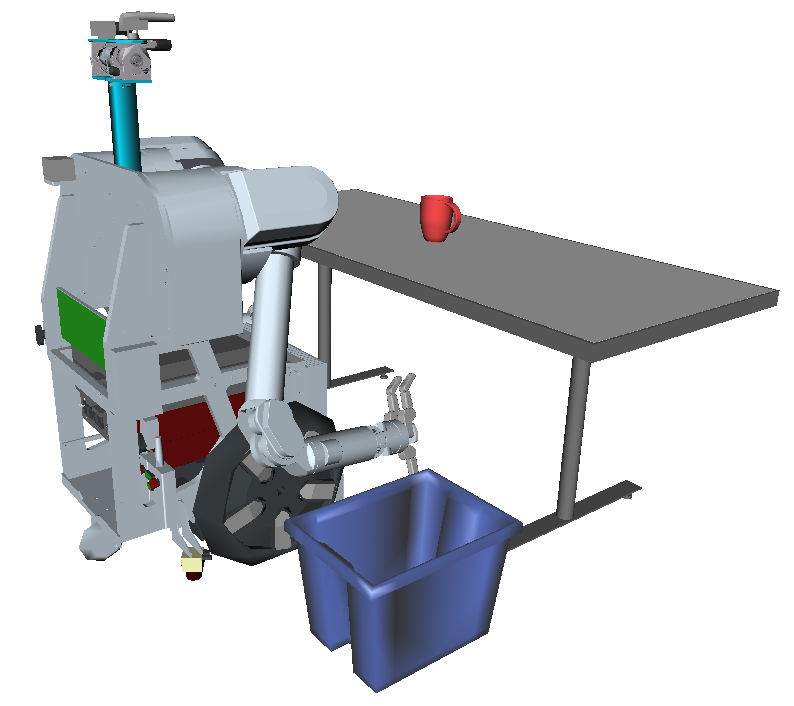
\includegraphics[width=0.45\textwidth]{figs/simple-table-clearing-task.png}
   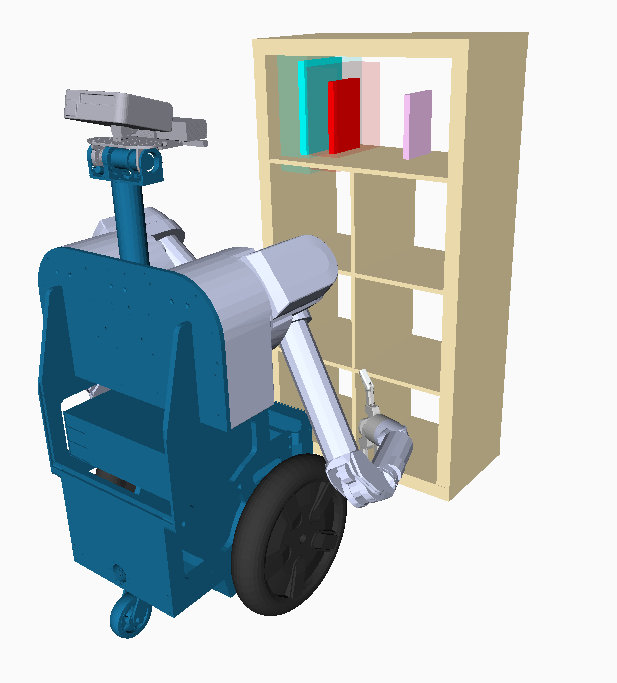
\includegraphics[width=0.45\textwidth]{figs/herbarm-traj0-t000.png}
   \caption{The HERB home robot experimental platform.}
   \label{fig:intro:platform-herb}
\end{marginfigure}

\begin{marginfigure}
   \centering
   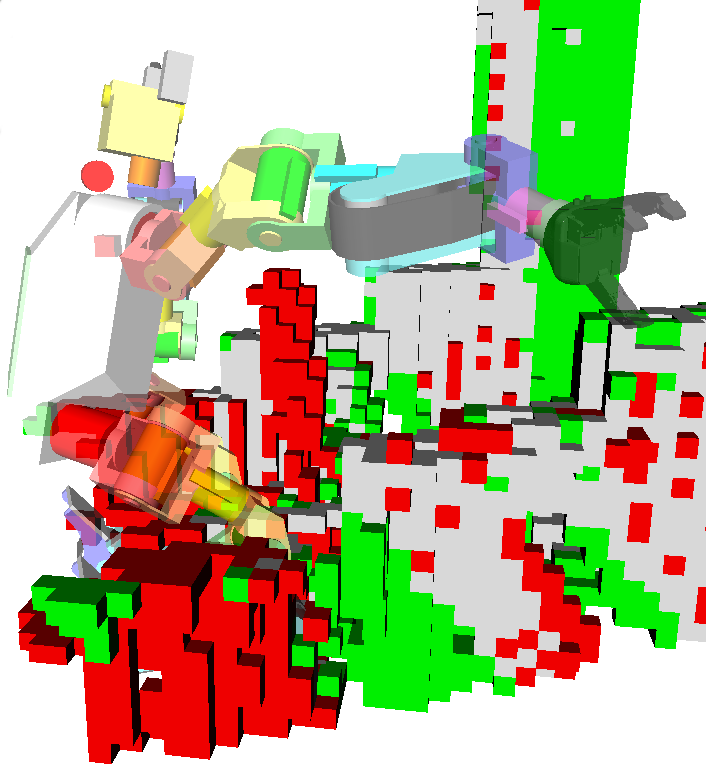
\includegraphics[width=0.8\textwidth]{figs/chimp-voxels-delta.png}
   \caption{The CHIMP disaster response robot.}
   \label{fig:intro:platform-chimp}
\end{marginfigure}

\begin{marginfigure}
   \centering
   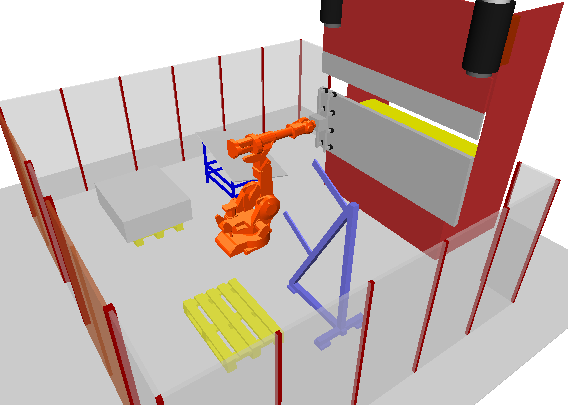
\includegraphics[width=\textwidth]{figs/workcell/config-a.png}
   \caption{An ABB IRB440 robot.}
   \label{fig:intro:platform-irb4400}
\end{marginfigure}



\chapter{Roadmap Methods for Motion Planning}
\label{chap:roadmaps}

Robots are fundamentally agents that move through the world,
and so the question of how to best deliberate about motion
is a central problem in robotics.
Different tasks and problem domains expose a vast array of
qualities and properties of motion that are important
-- for example, motion that is expressive, efficient, or expected
-- and algorithms can rely on a rich and growing set
of models and methodologies in order to generate such motion.

Underlying this rich tapestry of robotic motion
is the most fundamental abstraction of motion planning --
finding a path for a system which accomplishes a motion task
without colliding with obstacles.
While this might at first seem straightfoward,
finding such paths for articulated robotics in
complex semi-structured environments
is no easy feat,
and finding such paths quickly and efficiently
is of upmost importance.

This chapter includes a brief introduction to
the motion planning problem.
Due to its paramount importance to robotics,
variations on this problem have deservedly
enjoyed a considerable amount of attention over the past 40 years.
We tailor our investigation towards aspects of the problem
that are relevant to this thesis
-- for a comprehensive treatment,
we refer to LaValle \citep{lavalle2006planningbook}
and Choset et. al. \citep{choset2005robotmotion}.
In particular,
we provide an overview of a class of approaches called roadmap methods
that are well-suited to motion planning for articulated robots.

\section{The Motion Planning Problem}

\begin{marginfigure}
   \centering
   \includegraphics{build/movers-problem-schwartz-sharir} %
   \caption[The original mover's problem
      entails finding a collision-free path for a geometric body
      amongst obstacles,
      or finding that no path exists.
   ]{The original mover's problem
      \citep{schwartzsharir1983pianomovers1}
      entails finding a collision-free path for a geometric body
      amongst obstacles,
      or finding that no path exists.}
   \label{fig:roadmaps:movers}
\end{marginfigure}

The earliest studies of motion planning considered a single rigid
body moving within a Euclidean environment consisting of
fixed geometric obstacles
(Figure~\ref{fig:roadmaps:movers}).
Termed the \emph{FindPath} or \emph{piano mover's} problem,
this representation and variations thereof were extensively studied
\citep{lozanoperezwedley1979collisionfree,
   schwartzsharir1983pianomovers1},
for small dimensionalities (e.g. two or three)
and obstacle representations (e.g. polygonal regions).
Importantly,
these earlest problems exhibited two fundamental properties
inherent in all motion planning problems:
(a) that solutions,
called \emph{motions} or \emph{paths},
are continuous, and
(b) that the fundamental feasibility objective is binary,
with any prospective path either infeasible (in collision)
or feasible (collision-free).
The problem entails finding a feasible solution path if one exists,
or returning with failure otherwise.

\begin{marginfigure}
   \centering
   \includegraphics{build/c-space} %
   \caption{The motion planning problem entails finding a continuous
      path among obstacles in an abstract configuration space.}
   \label{fig:roadmaps:cspace}
\end{marginfigure}

\paragraph{The Configuration Space.}
A generalization of the piano mover's problem
commonly called the \emph{motion planning problem}
entails an abstraction of the single rigid body
to an arbitrary \emph{configuration space} (C-space)
\citep{lozanoperez1983cspace}.
Any point $q$ in this abstract space $\mathcal{C}$
(see Figure~\ref{fig:roadmaps:cspace})
corresponds to a full configuration of the system,
such as the position and orientation of a rigid body.
Importantly,
$\mathcal{C}$ can also capture the full configuration (or joint)
space of an articulated robotic manipulator.

Any point $q \in \mathcal{C}$ corresponds to a particular geometric
configuration of the robot within its fixed environment.
If this configuration results in a geometric collision in the workspace
(either between the robot and the environment,
or the robot with itself),
this point lies within a \emph{configuration-space obstacle},
e.g. $CO_1$ in Figure~\ref{fig:roadmaps:cspace}.
The union of these configurations comprises the set of obstacle
configurations $\mathcal{C}_{\ms{obs}}$,
and a configuration $q$ is collision free if
it is contained within the complement of this set
$\mathcal{C}_{\ms{free}} = \mathcal{C} \setminus \mathcal{C}_{\ms{obs}}$.

\paragraph{Paths in $\mathcal{C}$.}
A continuous function $\xi : [0,1] \rightarrow \mathcal{C}$
of bounded variation is called a \emph{path},
and let the set $\Xi$ denote the set of such paths.
We can then establish path validity:
\begin{equation}
   \mbox{path $\xi$ is valid} \iff
   \xi(t) \in \mathcal{C}_{\ms{free}} \;\forall t \in [0,1]
   \label{eqn:roadmaps:path-validity}
\end{equation}
We can capture this defininition for use in an optimization
framework via the functional
$x_{\ms{valid}} : \Xi \rightarrow \mathbb{R}$
shown in Figure~\ref{fig:roadmaps:cost-model-feasible}.

\begin{marginfigure}
   \centering
   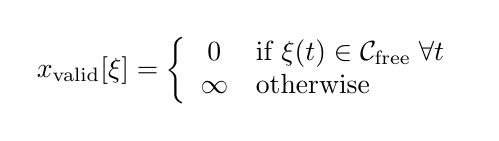
\begin{tikzpicture}
      \node at (0,0) {
         $\arraycolsep=5pt%
         x_{\ms{valid}}[\xi] = \left\{ \begin{array}{cl}
            0 & \mbox{if } \xi(t) \in \mathcal{C}_{\ms{free}} \;\forall t \\
            \infty & \mbox{otherwise} \\
         \end{array} \right.$
      };
   \end{tikzpicture}
   \caption{Edge cost model
      for the (feasible) motion planning problem.}
   \label{fig:roadmaps:cost-model-feasible}
\end{marginfigure}

\paragraph{The Motion Planning Problem.}
Consider a single-pair motion planning query $u$
consisting of start and destination vertices
$q_{\ms{start}}, q_{\ms{dest}} \in \mathcal{C}$
as well as a collision-free subset $\mathcal{C}_{\ms{free}}$.
The motion planning problem consists of finding a valid path $\xi^*$
with $\xi^*(0) = q_{\ms{start}}$ and $\xi^*(1) = q_{\ms{dest}}$
if one exists.

\subsection{Optimal Motion Planning}

\begin{marginfigure}
   \centering
   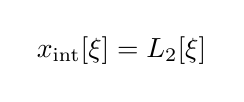
\begin{tikzpicture}
      \node at (0,0) {
         $x_{\ms{int}}[\xi] = L_2[\xi]$
      };
   \end{tikzpicture}
   \caption{Example dynamical cost function for the optimal
      motion planning problem.
      Here, the arc length of $\xi$ using the $L_2$ norm cost is used.}
   \label{fig:roadmaps:cost-model-path}
\end{marginfigure}

The \emph{optimal motion planning problem}
is a generalization of the motion planning problem which
includes an additional objective over solution paths
$x_{\ms{int}} : \Xi \rightarrow \mathbb{R}$
intended to measure properties intrinsic to the path.
Common choices for $x_{\ms{int}}$ include
the path's arc length,
the total time or energy necessary to execute the path,
or the squared time derivatives averaged over the path.
See \citep{karaman2011samplingoptimal} for a comprehensive treatment
of sampling-based methods for the optimal motion planning problem.

\marginnote{An optimal moption planner
   typically considers both feasibility dynamical properties of candidate paths --
   this objective is simply $x_{\ms{opt}} = x_{\ms{valid}} + x_{\ms{int}}$.
   We treat them separately because they exhibit fundamentally different
   computational profiles.}

\subsection{Further Generalizations}

There are a great number of further generalizations of the
motion planning problem that we will not explicitly consider.
For example,
the kinodynamic planning problem includes the derivatives of the
configuration variables,
and a solution to the kinodynamic problem is called a trajectory.
Various algorithms exist \citep{lavallekuffner1999rrt}.
The objective used in optimal variants of the kinodynamic problem
often include components which depend on the accelerations or torques
required to execute the trajectory.

Constrained motion planning constitutes an additional generalization.
A holonomic constraint on the configuration space,
for example,
induces a subset (often a manifold) of the configuration space
on which planning is restricted.
Various motion planners \citep{berenson2009manifolds}
have been proposed to accommodate such constraints.

\section{Motion Planning by Discretizing C-Space}

While the generalized mover's problem is computationally hard
\citep{reif1979moverscomplexity},
a large array of algorithms have been proposed that perform
well on a large range of typical instances.
We give a brief review of approaches to the motion planning problem
that rely principally on discretizations of the configuration space.

\subsection{Building Graphs in C-Space}
\label{subsec:roadmaps:building-graphs}

\paragraph{Testing Validity of Configurations}
How can we establish the validity of a configuration $q$?
This question is especially delicate when the geometry is complex
and the configuration-space obstacles cannot be represented explicitly.
In this case,
it is necessary to test prospective paths
for membership in $\mathcal{C}_{\ms{free}}$ using a predicate
that we express as a binary-valued
\emph{indicator function},
\begin{equation}
   \mathbf{1}_{\mathcal{C}\ms{free}} : \mathcal{C} \rightarrow
      \{ \mbox{True}, \mbox{False} \} 
   \mbox{\quad s.t. \quad}
   \mathbf{1}_{\mathcal{C}\ms{free}}(q) = \mbox{True} \mbox{ iff } q \in \mathcal{C}_{\ms{free}}.
\end{equation}
Note that implementing $\mathbf{1}_{\mathcal{C}\ms{free}}$ for an articulated robot
entails computing the forward kinematics of the robot at the
query configuration,
and conducting a collision check in the workspace.

\paragraph{Testing Validity of Paths}
How can we establish the validity of a path $\xi$
according to (\ref{eqn:roadmaps:path-validity})?
There are many approaches that can be applied,
including C-space bubbles \citep{quinlan1994modification}
and computing a path discretization resolution and corresponding
workspace obstacle padding
\citep{barraquand1991distributedrepresentation}.
We will generally assume that a functional variant of the indicator
function is available:%
\marginnote{The experiments in this document commit to a particular
collision checking resolution for motion validity.}%
\begin{equation}
   \mathbf{1}_{\Xi\ms{free}} : \Xi \rightarrow
      \{ \mbox{True}, \mbox{False} \} .
\end{equation}

\paragraph{Motion Planning as Pathfinding.}
Importantly,
two paths $\xi_{ab}$ and $\xi_{bc}$ with $\xi_{ab}(1) = \xi_{bc}(0)$
can be concatenated to a path $\xi_{ac}$,
with
\begin{equation}
   \mathbf{1}_{\Xi\ms{free}}(\xi_{ab})
   \;\land\;
   \mathbf{1}_{\Xi\ms{free}}(\xi_{bc})
   \iff
   \mathbf{1}_{\Xi\ms{free}}(\xi_{ac}).
\end{equation}
This motivates approaches which maintain a graph structure of
smaller valid motions in the configuration space.
Consider a graph $G = (V,E)$,
with each vertex $v \in V$ a configuration $q_v \in \mathcal{C}$,
and each edge $e_{uv} \in E$ a path $\xi_e \in \Xi$
s.t. $\xi(0) = q_u$ and $\xi(1) = q_v$,
and consider vertices $v_{\ms{start}}, v_{\ms{dest}} \in V$
corresponding to query vertices $q_{\ms{start}}, q_{\ms{dest}}$.
Then a path $p$ through $G$ from
$v_{\ms{start}}$ to $v_{\ms{dest}}$,
on which each edge $e$ has $\mathbf{1}_{\Xi\ms{free}}(\xi_e) = \mbox{True}$,
corresponds to a valid solution to the motion planning problem.

\paragraph{Optimal Motion Planning as Pathfinding.}
Furthermore,
if the intrinsic optimization objective $x_{\ms{int}}$
from Figure~\ref{fig:roadmaps:cost-model-path} is \emph{additive},
then the optimal motion planning problem can be solved on $G$
via a shortest path algorithm
(at least up to the discretization afforded by the graph).
This is accomplished by defining an edge weight function
$w : E \rightarrow \mathbb{R}$
by $w(e) = x_{\ms{opt}}(\xi_e)$.

A wide variety of approaches exist in the literature for
constructing, searching, and validating this graph
for motion planning problems.
We will broadly review a selection of different algorithms later
in this chapter (Section~\ref{sec:roadmaps:sensitivity}).

%\paragraph{Resolution and Probabalistic Completeness.}
%Any discretization is only an approximation of the actual configuration
%space.
%Of course, the discretization is always just an approximation
%of the actual C-space.
%Hopefully, you can choose a discretization strategy that allows your
%algorithm to have one or both of these forms of completeness.

%\paragraph{Motion Planning as Pathfinding.}
%\label{subsec:roadmaps:planning-as-pathfinding}
%Here, talk about how even if there are multiple available
%start or goal configurations
%(e.g. different grasps or inverse kinematics solutions),
%the motion planning problem can still be posed as a
%single-pair shortest path (SPSP) problem
%by augmenting the graph with virtual source sink vertices
%and edges.

\paragraph{Other Approaches to Motion Planning.}
The motion planning problem affords a number of different classes of
algorithms,
many of which do not construct graphs of local motions in the
problem's configuration space.
Potential field methods \citep{khatib1986potentialfields}
and navigation functions \citep{rimon1989navigationfunctions}
construct fields whose gradients can guide a path around
local obstacles.
Trajectory optimization approaches are especially well-suited to
planning instances in which the basins of attraction are large.
Approaches such as CHOMP \citep{zucker2013chomp}
and TrajOpt \citep{schulman2013trajopt})
commit to a trajectory representation for $\xi^{(1)}$
and use require stronger world descriptions
(SDFs, convex obstacle decompositions)
to make local modifications
to produce a new path $\xi^{(2)}$.
Also,
optimizers are commonly used in lower levels to react to local
changes (e.g. \citep{quinlan1994modification}).

\section{Obstacle Sensitivity}
\label{sec:roadmaps:sensitivity}

Generally,
graph-based motion approaches as described
in Section~\ref{subsec:roadmaps:building-graphs}
require the following three processes:
(a) constructing the graph,
(b) searching the graph, and
(c) validating the graph.
One of the key differentiators between the many graph-building
techniques for motion planning
is how they interleave these three processes.
This section considers one important factor:
the degree of dependence of the graph structure
on the distribution of obstacles in the scene.
We broadly categorize algorithms into two groups:
those that are \emph{obstacle-sensitive},
and those that are \emph{obstacle-insensitive}.

\subsection{Obstacle-Sensitive Approaches}
\label{subsec:roadmaps:sensitive}

In an obstacle sensitive approach,
the graph is built incrementally,
and construction of new elements (e.g. vertices and edges)
is directly interleaved with validating those elements
in response to the distribution of valid or costly states.
These approaches might be best understood
as constructing an approximation to $\mathcal{C}_{\ms{free}}$
as directly as possible.

\paragraph{Exact Algorithms.}
The earliest work on the motion planning problem studied
\emph{exact} or \emph{semi-algebraic}
algorithms which worked directly on an explicit representation
of the obstacles (e.g. polygons) in the configuration space
\citep{lozanoperez1983cspace}.
This formulation of motion planning was shown to be
PSPACE-hard \citep{reif1979moverscomplexity,canny1988complexitymotionplanning}.
These approaches can guarantee optimal solutions,
and may be even be able to guarantee the validity of certain edges
by construction.
However,
they are difficult to apply to problems on articulated
robots for two reasons.
First, many approaches are only applicable to problems
in two or three dimensions,
or to robots with only translational degrees of freedome
\citep{kavraki1995cspacefft}.
Second, an explicit representation of obstacles in the
configuration space is exceedingly difficult to achieve due to the
nonlinearity in the forward kinematics function.
While some approaches are able to construct explicit
analytical or approximate configuraion space obstacles from
workspace geometry (e.g. \citep{newmanbranicky1991cspacetransforms}),
they are often only applicable to simple kinematics.

\paragraph{Treebuilding Algorithms.}
Many approaches do treat the configuration space implicitly
(i.e. using indicator functions for validity checking as described
in Section~\ref{subsec:roadmaps:building-graphs}).
The most common algorithms simulteneously grow and validate trees,
either unidirectionally from the $v_{\ms{start}}$ or bidirectionally
from both start and goal configurations.
At each iteration,
these algorithms use a sampling strategy to propose a new extension,
and then augment their tree(s) if the new motion is found to be valid.
Key examples of this approach include
Expansive Space Trees (EST) \citep{hsu1997expansive}
and Rapidly-exploring Random Trees (RRT)
\citep{lavalle1998rrt, kuffner2000rrtconnect}.
The SBL planner \citep{sanchezante2001sbl}
is a bidirectional variant of EST with lazy edge validity checking.

\paragraph{Planning vs. Execution Cost.}
The foundational algorithms in this category are primarily concerned
with path \emph{feasibility} -- that is, the objective $x_{\ms{valid}}$
from Figure~\ref{fig:roadmaps:cost-model-feasible};
there is often no mechanism explicitly biasing them to select
low-cost paths.
\marginnote{We talk about this tradeoff between planning and
execution cost in detail in Chapter~\ref{chap:utility}.}
Therefore, solutions found tend to be of low quality,
and they are customarily optimized using a path shortcutting
algorithm in a post-processing phase before they can be executed.
More recent work has also focused on asymptotically optimal variants
of these planners
\citep{karaman2010rrtstar, karaman2011samplingoptimal, gammell2015bitstar, hauser2015lazy}
which do address more general cost objectives.

\paragraph{Advantages of Obstacle Sensitivity.}
One key advantage to obstacle-sensative approaches is that
they only construct the graph structure in the parts of the
configuration space that are relevant to the planning query.
The Vornoi sampling bias of the RRT or the importance sampling of the EST
attempt to focus graph construction in areas of the configuration space
which tend to find feasible paths quickly.
These techniques can also take account of the current distribution
and connectivity of the discretization in order to focus new
samples to their advantage
(e.g. to address the narrow passage problem),
such as visibility tests \citep{simeon2000visibilityprms}
or the expansion phase of the original PRM
\citep{kavrakietal1996prm}
or the visibility test of the Visibili
These heuristics can also be incorporated into sampling-based planners
as obstacle-based \citep{boor1999prmgaussiansampling}
or hybrid \citep{hsu2005hybridsampling} sampling strategies.

An additional advantage of these approaches
is that they handle densification naturally.
The graph structure is augmented automatically,
so the resolution of the discretization need not be explicitly
increased as the instance reveals itself to be more difficult.

%Probabalistic completeness.

\subsection{Obstacle-Insensitive Approaches}

In contrast to obstacle-sensitive approaches,
the approaches we describe here
commit to a particular discretization
of the configuration space a priori,
independent of the distribution of obstacles.
While this simpler method forgoes some of the advantages of
obstacle sensitivity discussed previously,
this idependence does confer some advantages of its own.

\paragraph{Roadmap Methods.}

The foundational obstacle-insensitive methods particular to the motion
planning problem are called \emph{roadmap methods}.
The term roadmap usually connotes a graph embedded in a continous
ambient space in the presence of obstacles.
Vertices in the graph,
which correspond to configurations in the configuration space,
are also called milestones.
The first roadmap methods such as the
Probabalistic RoadMap (PRM) \citep{kavrakietal1996prm}
initialized the milestones arrangement
from a uniform distribution over the free space.

Key to roadmap methods to motion planning
is the concept of the \emph{local planner}
which governs the validity of roadmap edges.
Given two configurations $q_a, q_b \in \mathcal{C}$,
the local planner considers a candidate path $\xi_{ab}$ between
them.
(A common implementation simply uses the straight-line path
in configuration space.)
Edges are only attempted when they meet certain restrictions,
such as distance with respect to some metric.

There are some variants of roadmap planners that are not independent
of the obstacle distribution.
First,
many roadmap planners make use of a heuristic ``expansion'' step
wherein additional samples are added to the roadmap
in order to increase its connectivity.
Second,
edge connection rules that can forgo connections within
the same connected component.

%\cdnote{Densification?}

\paragraph{Search-based Methods.}
Graph pathfinding algorithms such as A* \citep{hart1968astar}
are applicable to the motion planning problem if a suitable
discretization of the continuous space is considered.
While roadmaps can serve as this discretization,
application of search-based methods often represents the space
implicitly via a set of operators or motion primitives
which reproduce a regular lattice over the configuration space
\citep{pivtoraiko2005statelattice}.
When the vertices comprising the lattice are rectangular
(also called a Sukharev point set \citep{sukharev1971extremum}),
seach-based planning is also called ``grid search.''

\paragraph{Lazy Validity Checking.}
Because obstacle-insensitive approaches decouple graph construction
from validity checking,
it is often advantageous to defer the latter until it is
necessary for solving the query at hand.
Lazy validity checking has been exploited
in roadmap methods such as the Lazy PRM
\citep{bohlin2000lazyprm, hauser2015lazy},
search methods such as Lazy Weighted A* \citep{cohen2014narms},
and methods which bridge the two
such as Fast Marching Trees (FMT*) \citep{janson2015fmtstar}
and Bidirectional FMT* (BFMT*) \citep{starek2015bfmtstar}.
We discuss laziness in the context of graph search
more comprehensively in Chapter~\ref{chap:lazysp}

\paragraph{Adaptive Densification.}
One difficulty with these obstacle-insensitive approaches
is that they commit to a particular discretization,
and once their search is exhausted,
they must return the best path found,
or report failure if no path was found.
This property is known as resolution completeness
\citep{cheng2004rescomplete}.

Many instance of prior work endeavor to progressively
densify their discretization until a suitable solution is found.
Early examples of this approach include
hierarchical cell decompositions \citep{faverjon1984octree}
and workspace and C-space bitmap pyramids for search over potential fields
\citep{barraquand1991distributedrepresentation}.
More recent asymptotically optimal motion planners such as
Lazy PRM* \citep{hauser2015lazy}.
and BIT* \citep{gammell2015bitstar} take a similar approach to
roadmap search,
which we also adopt as described in Chapter~\ref{chap:utility}
(see Figure~\ref{fig:roadmaps:roadmap-stack}).

\begin{figure}
   \centering
   \includegraphics{build/roadmap-stack}
   \caption{A stack of progressively densified roadmaps
      over a given configuration space $\mathcal{C}$.
      Each deeper roadmap constitutes a more accurate approximation
      to the true continuous problem space.}
   \label{fig:roadmaps:roadmap-stack}
\end{figure}

\paragraph{Advantages of Obstacle Insensitivity.}
The obstacle sensitivity question represents an underlying efficiency
tradeoff.
Sensitive approaches may be able to adapt their discretization more
directly to local obstacle distributions.
On the other hand,
insensitivity to obstacles admits a number of efficiency advantages.
Much of the nearest-neighbor computation
often required during graph construction can be cached and amortized
over all planning queries.
Other properties of the discretization that are constant between
similar planning instances can also be shared
as described in Chapter~\ref{chap:family}.
For these reasons,
this thesis build on top of obstacle-insensitive roadmaps.

\section{Roadmap Classes}
\label{sec:roadmaps:roadmap-classes}

Roadmap methods operate over a graph constructed in the
robot's configuration space.
Roadmap miletones are commonly genererated by a number of different
types of point sequences,
and edges are considered between vertices pairs that meet
certain constraints.
While most algorithms methods are generally agnostic
to the class of roadmap that they operate on,
choosing a suitable class and its parameters has a large effect
on both theoretical and practical perforamce.

\paragraph{Random Sequences.}
The original roadmap algorithms
\citep{kavrakietal1996prm}
operated primarily over sets
of vertices drawn uniformly at random from the configuration space.
Many more recent algorithms such as
RRT* \citep{karaman2010rrtstar},
PRM* \citep{karaman2011samplingoptimal},
FMT* \citep{janson2015fmtstar},
RRT$^{\#}$ \citep{arslan2013rrtsharp},
and BIT* \citep{gammell2015bitstar} make use of the same
uniform obstacle distribution.
Such a distribution is attractive both because
it is simple to implement
it because it allows for theoretical properties such as
completeness and optimality to be demonstrated
in probability.

\paragraph{Deterministic Sequences.}
Many researchers have examined whether randomness is a necessary
(or even beneficial) aspect of treebuilding and roadmap planners
\citep{branicky2002detvsprobroadmaps}.
This is especially relevant in the context of comparing
roadmap planners with search-based methods
that conventionally operate over lattices \citep{lavalle2002gridprms}.

One of the most straightforward disadvantages of using a
non-deterministic sequence for each motion planning query
is that the constructed graph is different for each query.
This makes it impractical to pre-compute and amortize nearest
neighbor queries across problem instances,
as well as to pre-compute edge states as decribed in
Chapter~\ref{chap:family}.

Further,
theoretical properties of roadmap methods
such as resolution completeness and asymptotic optimality
depend on properties of the underlying point set
such as its \emph{dispersion}.
Not only can the dispersion of a set of randomly sampled points
only be established in expectation,
but it is demonstrably larger than the dispersion of other
well-known point sequences,
such as the Halton or Hammersley set,
or the Sukharev grid.
For an in-depth analysis of differet point sets for roadmap
planning, see Janson \citep{janson2015deterministicsampling}.

\begin{figure}
   \centering
   \includegraphics{build/roadmaps/gen/aagrid}
   \;
   \includegraphics{build/roadmaps/gen/rgg}
   \;
   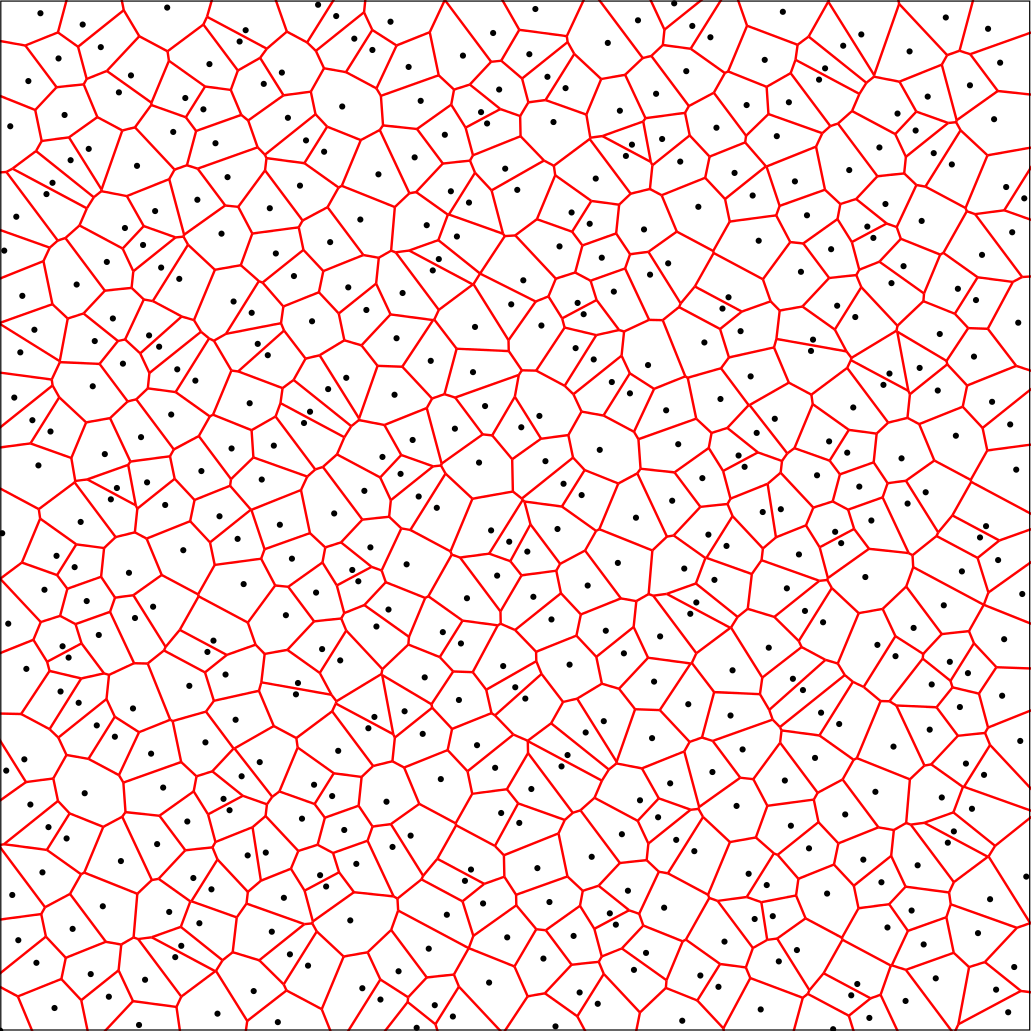
\includegraphics{build/roadmaps/gen/halton}
   \caption{Examples of three roadmap types over the unit square:
      an axis-aligned lattice (left),
      random geometric graph (middle),
      and Halton graph with primes $(2,3)$ (right).
      All three roadmaps have a connection radius of 0.3.
      The latter two roadmaps have 30 vertices.}
\end{figure}

\paragraph{Connection Radii.}
Previous work \citep{karaman2011samplingoptimal} has established
that a roadmap planner which uses a uniformly randomly generated
point set is asymptotically optimal almost surely
if the edge connection radius $r$ is sufficiently large w.r.t.
the number the number of samples $n$.
In particular,
it defines the critical value $\gamma^*_{\mathcal{C}}$:
\begin{equation}
   \gamma^*_{\mathcal{C}}
      = 2 \left( \left[ 1 + \frac{1}{d} \right]
         \frac{\lambda_d(\mathcal{C})}{\zeta_d} \right)^{1/d},
\end{equation}
where $d$ is the dimensionality of the configuration space,
$\lambda_d(\cdot)$ represents the Lebesgue measure (e.g. volume),
and $\zeta_d$ is the Lebesgue measure of the $d$-dimensional unit ball.
Note that while other publications consider $n$ to be the number
of milestones in the collision-free subset of the space
(and therefore also rely on the measure of that subset),
we measure the volume of the entire C-space,
and let $n$ correspond to the total number of vertices.
We do this because we will be determining the validity of roadmap edges
in a separate step,
as described in Chapter~\ref{chap:lazysp}.

Asymptotic optimality under uniform sampling requires
an edge connection radius $r_{\ms{log}}$:
\begin{equation}
   r_{\ms{log}}(n) =  \gamma^*_{\mathcal{C}} \, \eta
      \left( \frac{\log(n)}{n} \right)^{1/d}
\end{equation}
for some tuning parameter $\eta > 1$.
Point sets with tighter dispersion bounds,
such as the Halton sequence,
can exploit a smaller connection radius $r_{\ms{loglog}}$:
\begin{equation}
   r_{\ms{loglog}}(n) = \gamma_{\mathcal{C}} \, \eta
      \left( \frac{\log(\log(n))}{n} \right)^{1/d}.
\end{equation}
For details we refer the reader
to \citep{janson2015deterministicsampling}.

\begin{margintable}
   \centering
   {\renewcommand{\tabcolsep}{0.15cm}
   \begin{tabular}{lccc}
      \toprule
      & HERB & CHIMP & IRB 4400 \\
      \midrule
      $d$ & 7 & 7 & 6 \\
      $\gamma^*_{\mathcal{C}}$ & 7.67 & 7.97 & 7.74 \\
      $r_{\ms{log}}$ & 2.83 & 2.93 & 2.41 \\
      $r_{\ms{loglog}}$ & 2.31 & 2.40 & 1.90 \\
      \bottomrule
   \end{tabular}
   }
   \vspace{0.1cm}
   \caption{Table of roadmap connection radii parameters for
      various scaling rates across the different robot platforms
      considered in this thesis.
      Radii presented are for $n=10000$ and $\eta = 1$,
      and are given in radians.}
   \label{table:roadmap-params}
\end{margintable}

\paragraph{Roadmaps for Articulated Robots.}
We apply roadmap methods to the three robot platforms
from Chapter~\ref{chap:intro} in this thesis.
Unless otherwise noted,
we build roadmaps directly in the joint space of the robot.
See Table~\ref{table:roadmap-params} for the roadmap parameters
that we use.

%\cdnote{Add a plot of roadmap sizes for each batch
%for each robotic platform}.

%\subsection{Dispersion}
%
%Deterministic sampling and dispersion:
%\citep{janson2015deterministicsampling}.
%
%\begin{figure}
%   \centering
%   \includegraphics{build/roadmaps-dispersion/dispersion}
%   \caption{Dispersion plot on the unit square.
%      Green is the dispersion of an incremental (greedy) Sukharev
%      grid.}
%\end{figure}
%
%\begin{figure}
%   \centering
%   \includegraphics{build/roadmaps-dispersion/dispersion-herb}
%   \caption{HERB dispersion plot.}
%\end{figure}
%
%\begin{figure}
%   \centering
%   \includegraphics{build/roadmaps-dispersion/dispersion-irb4400}
%   \caption{IRB4400 dispersion plot.}
%\end{figure}

%\subsection{Batch Size}
%
%\begin{figure}
%   \centering
%   \begin{tikzpicture}
%   \begin{axis}[
%         xmode=log,
%         xlabel={Batch Size},
%         ylabel={LazySP Time (s)},
%         xlabel near ticks,
%         ylabel near ticks,
%         ]
%      \addplot coordinates {
%         (100, 0.2407595708)
%         (250, 0.27367886569999994)
%         (1000, 0.2165730066)
%         (2500, 0.3836524094)
%         (10000, 0.47772694290000006)
%      };
%   \end{axis}
%   \end{tikzpicture}
%   \caption{Batch size. {\tt herbbin0}, seeds 1-10, gammafac=1, lambda=0.}
%\end{figure}

\chapter{Fast Pathfinding on Graphs via Lazy Evaluation}
\label{chap:lazysp}

The roadmap methods described in Chapter~\ref{chap:roadmaps}
create a discretization of the configuration space by way of
a graph $G = (V,E)$.
This allows the motion planning problem to be solved by way of
a pathfinding algorithm on $G$
-- and there are a large variety of such algorithms available
in the literature to choose from.
However,
the computational efficiency of suitable algorithms
depends intimately on the underlying problem domain.

In this chapter,
we consider the general shortest path problem
with a particular focus on domains (such as robot motion planning)
where evaluating the edge weight function
dominates algorithm running time.
Inspired by lazy approaches in robotics,
we define and investigate the \emph{Lazy Shortest Path} class of
algorithms which is differentiated by the choice of
an \emph{edge selector} function.
We show that several algorithms in the literature are equivalent to
this lazy algorithm for appropriate choice of this selector.
Further, we propose various novel selectors inspired by
sampling and statistical mechanics,
and find that these selectors outperform
existing algorithms on a set of example problems.

\begin{figure}
\centering
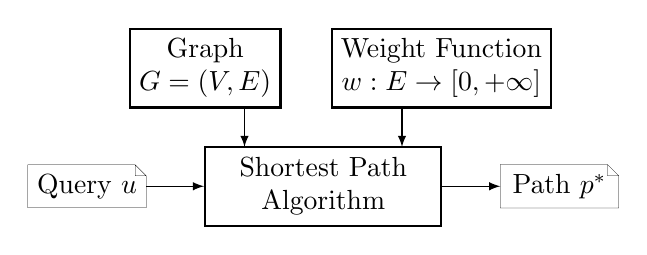
\begin{tikzpicture}
   \tikzset{>=latex} % arrow heads
   %\draw[step=1cm,black!10,very thin] (0,0) grid (8,4);
   \node[draw,align=center,minimum height=1.0cm,thick]
      at (2.5,2.5) {Graph\\$G=(V,E)$};
   \node[draw,align=center,minimum height=1.0cm,thick]
      at (5.5,2.5) {Weight Function\\$w:E \rightarrow [0,+\infty]$};
   \node[draw,align=center,minimum height=1.0cm,minimum width=3cm,thick]
      (alg) at (4,1) {Shortest Path\\Algorithm};
   \node[draw,align=center,shape=document,minimum width=1.5cm,ultra thin]
      (query) at (1,1) {Query $u$};
   \node[draw,align=center,shape=document,minimum width=1.5cm,ultra thin]
      (path) at (7,1) {Path $p^*$};
   \draw[->] (3,2) -- (3,1.5);
   \draw[->] (5,2) -- (5,1.5);
   \draw[->] (query.east) -- (alg.west);
   \draw[->] (alg.east) -- (path.west);
\end{tikzpicture}
\caption{While solving a shortest path query,
   a shortest path algorithm incurs computation cost from three sources:
   examining the structure of the graph $G$,
   evaluating the edge weight function $w$,
   and maintaining internal data structures.}
\label{fig:sp-intro}
\end{figure}

\section{The Shortest Path Problem}

Graphs provide a powerful abstraction
capable of representing problems in a wide variety of domains
from computer networking to puzzle solving
to robotic motion planning.
%\ajnote{Way too vague and general -- disconnected from second sentence.
%Maybe mention ``standard problems'' on graphs.}
In particular,
many important problems can be captured
as \emph{shortest path problems} (Figure~\ref{fig:sp-intro}),
wherein a path $p^*$ of minimal length is desired
between two query vertices through a graph $G$
with respect to an edge weight function $w$.
%As such,
%a large number of algorithms have been proposed in the literature
%for solving shortest path problems efficiently.

Despite the expansive applicability of this single abstraction,
there exist a wide variety of algorithms in the literature
for solving the shortest path problem efficiently.
%\ajnote{You say ``despite'' but the second part seems to follow from
%the first.
%There are many solutions because there are many problems.}
This is because the measure of computational efficiency,
and therefore the correct choice of algorithm,
is inextricably tied to the underlying problem domain.

The computational costs incurred by an algorithm
can be broadly categorized into three sources
corresponding to the blocks in Figure~\ref{fig:sp-intro}.
One such source consists of queries on the structure
of the graph $G$ itself.
The most commonly discussed such operation,
\emph{expanding} a vertex (determining its successors),
is especially fundamental
%\ajnote{especially costly?}
when the graph is represented implicitly,
e.g. for domains with large graphs
such as the 15-puzzle or Rubik's cube.
It is with respect to vertex expansions
that A* \citep{hart1968astar} is optimally efficient.

A second source of computational cost consists of maintaining
ordered data structures inside the algorithm itself,
which is especially important for problems with large branching
factors.
For such domains,
approaches such as partial expansion \citep{yoshizumi2000peastar}
or iterative deepening \citep{korf1985idastar}
significantly reduce the number of vertices generated and stored
by either selectively filtering surplus vertices from the frontier,
or by not storing the frontier at all.

The third source of computational cost arises not from reasoning
over the structure of $G$,
but instead from evaluating the edge weight function $w$
(i.e. we treat discovering an out-edge and determining its weight
separately).
Consider for example the problem of articulated robotic motion planning
using roadmap methods \citep{kavrakietal1996prm}.
While these graphs are often quite small
(fewer than $10^5$ vertices),
determining the weight of each edge requires performing many
collision and distance computations for the complex geometry
of the robot and environment,
resulting in planning times of multiple seconds to find a path.

As described in Chapter~\ref{chap:roadmaps},
we consider problem domains in which evaluating the edge weight
function $w$ dominates algorithm running time.
In this chapter,
we investigate the following research question:
\begin{quote}
How can we minimize the number of edges we need to evaluate
to answer shortest-path queries?
\end{quote}

We make three primary contributions.
First,
inspired by lazy collision checking techniques from 
robotic motion planning \citep{bohlin2000lazyprm},
we formulate a class of shortest-path algorithms 
that is well-suited to problem domains with expensive edge evaluations.
Second,
we show that several existing algorithms in the literature
can be expressed as special cases of this algorithm.
Third,
we show that the extensibility afforded by the algorithm allows for
novel edge evaluation strategies,
which can outperform existing algorithms
over a set of example problems.

\section{Lazy Shortest Path Algorithm}

We describe a lazy approach to finding short paths
which is well-suited to domains with
expensive edge evaluations.

\subsection{Problem Definition}

A path $p$ in a graph $G = (V,E)$
is composed of a sequence of adjacent edges 
connecting two endpoint vertices.
Given an edge weight function
$w : E \rightarrow [0,+\infty]$,
the length of the path with respect to $w$ is then:
\begin{equation}
   \mbox{len}(p, w) = \sum_{e \in p} w(e).
   \label{eqn:lazysp:len-definition}
\end{equation}
Given a single-pair planning query
$u: (v_{\ms{start}}, v_{\ms{goal}})$
inducing a set of satisfying paths $P_u$,
the \emph{shortest-path problem} is:
\begin{equation}
   p^* = \argmin_{p \, \in \, P_u} \mbox{len}(p, w).
   \label{eqn:objective}
\end{equation}

A shortest-path algorithm computes $p^*$
given $(G, u, w)$.
Many such algorithms have been proposed
to efficiently accommodate a wide array of underlying problem domains.
%(outlined in Section~\ref{sec:discussion}).
The well-known principle of best-first search (BFS)
is commonly employed to select vertices for expansion
so as to minimize such expansions while guaranteeing optimality.
Since we seek to minimize edge evaluations,
we apply BFS to the question of selecting candidate paths in
$G$ for evaluation.
The resulting algorithm, Lazy Shortest Path (LazySP),
is presented in Algorithm~\ref{alg:lazy-outline},
and can be applied to graphs defined implicitly or explicitly.

%\cdnote{To Sidd: You might not like this paragraph -- but I feel like
%going directly from the problem definition to the algorithm doesn't
%connect to the rationale strongly enough without it.
%What do you think?}

\subsection{The Algorithm}

\begin{algorithm}[t]
\caption{Lazy Shortest Path (LazySP)}
\label{alg:lazy-outline}
\begin{algorithmic}[1]
\Function {\textsc{LazyShortestPath}}{$G, u, w, w_{\ms{est}}$}
\State $E_{\ms{eval}} \leftarrow \emptyset$ %\Comment Initialize evaluated edges to empty
\State $w_{\ms{lazy}}(e) \leftarrow w_{\ms{est}}(e) \quad \forall e \in E$ %\Comment Initialize lazy edge weights to estimate (inexpensive)
\Loop
   \State $p_{\ms{candidate}} \leftarrow
      \mbox{\sc ShortestPath}(G, u, w_{\ms{lazy}})$ %\Comment Compute the shortest path with lazy edge weights
      \label{line:lazy-outline-shortestpath}
   \If {$p_{\ms{candidate}} \subseteq E_{\ms{eval}}$} %\Comment If all edges on path have already been evaluated,
      \State \Return $p_{\ms{candidate}}$ %\Comment path returned is provably optimal
   \EndIf
   \State $E_{\ms{selected}} \leftarrow  \mbox{\sc Selector}(G, p_{\ms{candidate}})$ %\Comment Select edges on path to process
   \label{line:lazy-outline-chooseedges} 
   \For {$e \in E_{\ms{selected}} \setminus E_{\ms{eval}}$} %\Comment For all unevaluated selected edges
      \State $w_{\ms{lazy}}(e) \leftarrow w(e)$ \Comment Evaluate (expensive)
      \State $E_{\ms{eval}} \leftarrow E_{\ms{eval}} \cup e$ %\Comment Add to evaluated edge set
   \EndFor
\EndLoop
\EndFunction
\end{algorithmic}
\end{algorithm}

We track evaluated edges with the set $E_{\ms{eval}}$.
We are given an estimator function $w_{\ms{est}}$ of the true edge weight $w$.
This estimator is inexpensive to compute
(e.g. edge length or even $0$).
We then define a \emph{lazy} weight function $w_{\ms{lazy}}$
which returns the
true weight of an evaluated edge and otherwise
uses the inexpensive estimator $w_{\ms{est}}$.

At each iteration of the search,
the algorithm uses $w_{\ms{lazy}}$ to compute a candidate path
$p_{\ms{candidate}}$
by calling an existing solver \textsc{ShortestPath}
(note that this invocation requires no evaluations of $w$).
Once a candidate path has been found,
it is returned if it is fully evaluated.
Otherwise,
an \emph{edge selector} is employed which selects
graph edge(s) for evaluation.
The true weights of these edges are then evaluated
(incurring the requisite computational cost),
and the algorithm repeats.

%\subsection{Theoretical Properties}

LazySP is complete and optimal
(proofs in the appendix):

\begin{theorem}[Completeness of LazySP]
If the graph $G$ is finite,
\textsc{ShortestPath} is complete,
and the set $E_{\ms{selected}}$
returned by \textsc{Selector}
returns at least one unevaluated edge on $p_{\ms{candidate}}$,
then \textsc{LazyShortestPath} is complete.
\label{thm:lazy-completeness}
\end{theorem}

\begin{theorem}[Optimality of LazySP]
If $w_{\ms{est}}$ is chosen such that
$w_{\ms{est}}(e) \leq \epsilon \, w(e)$ for some parameter
$\epsilon \geq 1$ and
\textsc{LazyShortestPath} terminates
with some path $p_{\ms{ret}}$,
then $\mbox{len}(p_{\ms{ret}}, w) \leq \epsilon \, \ell^*$
with $\ell^*$ the length of an optimal path.
\label{thm:lazy-optimality}
\end{theorem}

The optimality of LazySP depends on the admissibility of
$w_{\ms{est}}$
in the same way that the optimality of A* depends on
the admissibility of its goal heuristic $h$.
Theorem~\ref{thm:lazy-optimality} establishes the general
bounded suboptimality of LazySP
w.r.t. the inflation parameter $\epsilon$.
While our theoretical results (e.g. equivalences)
hold for any choice of $\epsilon$,
for clarity our examples and experimental results
focus on cases with $\epsilon = 1$.

\subsection{The Edge Selector: Key to Efficiency}

\begin{algorithm}[t]
\caption{Various Simple LazySP Edge Selectors}
\begin{algorithmic}[1]
\Function {\textsc{SelectExpand}}{$G, p_{\ms{candidate}}$}
   \State $e_{\ms{first}} \leftarrow$ first unevaluated $e \in p_{\ms{candidate}}$
   \State $v_{\ms{frontier}} \leftarrow G.\mbox{source}(e_{\ms{first}})$
   \State $E_{\ms{selected}} \leftarrow G.\mbox{out\_edges}(v_{\ms{frontier}})$
   \State \Return $E_{\ms{selected}}$
\EndFunction
\vspace{0.02in}
\Function {\textsc{SelectForward}}{$G, p_{\ms{candidate}}$}
   \State \Return $\{ \mbox{first unevaluated } e \in p_{\ms{candidate}} \}$
\EndFunction
\vspace{0.02in}
\Function {\textsc{SelectReverse}}{$G, p_{\ms{candidate}}$}
   \State \Return $\{ \mbox{last unevaluated } e \in p_{\ms{candidate}} \}$
\EndFunction
\vspace{0.02in}
\Function {\textsc{SelectAlternate}}{$G, p_{\ms{candidate}}$}
   \If {LazySP iteration number is odd}
      \State \Return $\{ \mbox{first unevaluated } e \in p_{\ms{candidate}} \}$
   \Else
      \State \Return $\{ \mbox{last unevaluated } e \in p_{\ms{candidate}} \}$
   \EndIf
\EndFunction
\vspace{0.02in}
\Function {\textsc{SelectBisection}}{$G, p_{\ms{candidate}}$}
   \State \Return $\left\{ \begin{array}{ll}
      \mbox{unevaluated } e \in p_{\ms{candidate}} \\
      \mbox{furthest from nearest evaluated edge}
      \end{array} \right\}$
\EndFunction
\end{algorithmic}
\label{alg:simple-selectors}
\end{algorithm}

%The algorithm purposely leaves undecided
%the edge evaluation selector codified in
%\textsc{Selector} (line~\ref{line:lazy-outline-chooseedges}),
%and therefore describes a class of algorithms
%differentiated by the choice of this selector.
%This paper discusses particular choices.

The LazySP algorithm exhibits a rough similarity to optimal
replanning algorithms such as
D* \citep{stentz1994dstar} \citep{stentz1995focusseddstar}
which plan a sequence of shortest paths for a mobile robot
as new edge weights are discovered during its traverse.
D* treats edge changes
passively as an aspect of the problem setting
(e.g. a sensor with limited range).

The key difference is that our problem setting treats 
edge evaluations as an active choice that can be exploited.
While any choice of edge selector that meets the conditions above
will lead to an algorithm that is complete and optimal,
its \emph{efficiency} is dictated by the choice of this
selector.
This motivates the theoretical and empirical investigation of different
edge selectors in this chapter.

\textbf{Simple selectors.}
We codify five common strategies in
Algorithm~\ref{alg:simple-selectors}.
The Expand selector captures the edge weights that are evaluated
during a conventional vertex expansion.
The selector identifies the first unevaluated edge
$e_{\ms{first}}$ on the candidate path,
and considers the source vertex of this edge a \emph{frontier} vertex.
It then selects all out-edges of this frontier vertex
for evaluation.
The Forward and Reverse selectors select the first and last
unevaluated edge on the candidate path, respectively
(note that Forward returns a subset of Expand).

The Alternate selector simply alternates between Forward
and Reverse on each iteration.
This can be motivated by both bidirectional search algorithms
as well as motion planning algorithms such as
RRT-Connect \citep{kuffner2000rrtconnect}
which tend to perform well w.r.t. state evaluations.

The Bisection selector
chooses among those unevaluated edges
the one furthest from an evaluated edge on the candidate path.
This selector is roughly analogous to the collision checking strategy
employed by the Lazy PRM \citep{bohlin2000lazyprm}
as applied to our problem on abstract graphs.

In the following section,
we demonstrate that instances of LazySP using simple selectors
yield equivalent results to existing vertex algorithms.
We then discuss two more sophisticated
selectors motivated by weight function sampling
and statistical mechanics.

% prob-box2d00-halton-roots16
% fwd:34 partall:22 rev:24 fwdexpand:77
% bisect:25 worlddist:22 alt:23 partsimple:22
\begin{figure*}[t!]%
   \!\!%
   \subfloat[Expand(77)]{%
      \centering%
      \begin{tikzpicture}
         \node at (0,-0.0) {\includegraphics{build/lazysp-example-1/alg-fwdexpand-after5}};
         \node at (0,-2.5) {\includegraphics{build/lazysp-example-1/alg-fwdexpand-end}};
         \node at (0,-4.8) {\includegraphics{build/lazysp-example-1/alg-fwdexpand-path-bars}};
      \end{tikzpicture}%
   }%
   \!\!%
   \subfloat[Forward(34)]{%
      \centering%
      \begin{tikzpicture}
         \node at (0,-0.0) {\includegraphics{build/lazysp-example-1/alg-fwd-after5}};
         \node at (0,-2.5) {\includegraphics{build/lazysp-example-1/alg-fwd-end}};
         \node at (0,-4.8) {\includegraphics{build/lazysp-example-1/alg-fwd-path-bars}};
      \end{tikzpicture}%
   }%
   \!\!%
   \subfloat[Reverse(24)]{%
      \centering%
      \begin{tikzpicture}
         \node at (0,-0.0) {\includegraphics{build/lazysp-example-1/alg-rev-after5}};
         \node at (0,-2.5) {\includegraphics{build/lazysp-example-1/alg-rev-end}};
         \node at (0,-4.8) {\includegraphics{build/lazysp-example-1/alg-rev-path-bars}};
      \end{tikzpicture}%
   }%
   \!\!%
   \subfloat[Alternate(23)]{%
      \centering%
      \begin{tikzpicture}
         \node at (0,-0.0) {\includegraphics{build/lazysp-example-1/alg-alt-after5}};
         \node at (0,-2.5) {\includegraphics{build/lazysp-example-1/alg-alt-end}};
         \node at (0,-4.8) {\includegraphics{build/lazysp-example-1/alg-alt-path-bars}};
      \end{tikzpicture}%
   }%
   \!\!%
   \subfloat[Bisect(25)]{%
      \centering%
      \begin{tikzpicture}
         \node at (0,-0.0) {\includegraphics{build/lazysp-example-1/alg-bisect-after5}};
         \node at (0,-2.5) {\includegraphics{build/lazysp-example-1/alg-bisect-end}};
         \node at (0,-4.8) {\includegraphics{build/lazysp-example-1/alg-bisect-path-bars}};
      \end{tikzpicture}%
   }%
   \!\!%
   \subfloat[WeightSamp(22)]{%
      \centering%
      \begin{tikzpicture}
         \node at (0,-0.0) {\includegraphics{build/lazysp-example-1/alg-worlddist1000-after5}};
         \node at (0,-2.5) {\includegraphics{build/lazysp-example-1/alg-worlddist1000-end}};
         \node at (0,-4.8) {\includegraphics{build/lazysp-example-1/alg-worlddist1000-path-bars}};
      \end{tikzpicture}%
   }%
   \!\!%
   \subfloat[Partition(22)]{%
      \centering%
      \begin{tikzpicture}
         \node at (0,-0.0) {\includegraphics{build/lazysp-example-1/alg-partall-after5}};
         \node at (0,-2.5) {\includegraphics{build/lazysp-example-1/alg-partall-end}};
         \node at (0,-4.8) {\includegraphics{build/lazysp-example-1/alg-partall-path-bars}};
      \end{tikzpicture}%
   }%
   \caption[Snapshots of the LazySP algorithm using each edge selector
      discussed in this chapter on the same obstacle roadmap graph problem,
      with start and goal.
      At top, the algorithms after evaluating five edges
      (evaluated edges labeled as valid or invalid).
      At middle, the final set of evaluated edges.
      At bottom, for each unique path considered from left to right,
      the number of edges on the path that are
      already evaluated, evaluated and valid, evaluated and invalid,
      and unevaluated.
      The total number of edges evaluated is noted in brackets.
      Note that the scale on the Expand plot has been adjusted
      because the selector evaluates many edges not on the candidate
      path at each iteration.
   ]{Snapshots of the LazySP algorithm using each edge selector
      discussed in this chapter on the same obstacle roadmap graph problem,
      with start (\protect\tikz[baseline=-0.5ex]{\protect\node[circle,fill=blue,inner sep=1pt]{};})
      and goal (\protect\tikz[baseline=-0.5ex]{\protect\node[circle,fill=green,inner sep=1pt]{};}).
      At top, the algorithms after evaluating five edges
      (evaluated edges labeled as
      \protect\tikz{\protect\draw[very thick] (0,0) -- (0.15,0.15);}  valid
      or \protect\tikz{\protect\draw[very thick,red] (0,0) -- (0.15,0.15);} invalid).
      At middle, the final set of evaluated edges.
      At bottom, for each unique path considered from left to right,
      the number of edges on the path that are
      \protect\tikz{\protect\node[fill=green!40!white,draw=black]{};}\;already evaluated,
      \protect\tikz{\protect\node[fill=green!70!black,draw=black]{};}\;evaluated and valid,
      \protect\tikz{\protect\node[fill=red!70!black,draw=black]{};}\;evaluated and invalid,
      and \protect\tikz{\protect\node[fill=black!10!white,draw=black]{};}\;unevaluated.
      The total number of edges evaluated is noted in brackets.
      Note that the scale on the Expand plot has been adjusted
      because the selector evaluates many edges not on the candidate
      path at each iteration.
      }
   \label{fig:snapshots}
\end{figure*}

\section{Edge Equivalence to A* Variants}

In the previous section,
we introduced LazySP as the path-selection analogue
to BFS vertex-selection algorithms.
In this section,
we make this analogy more precise.
In particular,
we show that LazySP-Expand
%(that is, LazySP with the Expand selector)
%\ajnote{name consistency}
is edge-equivalent to a variant of A*
(and Weighted A*),
and that LazySP-Forward is edge-equivalent to a variant of
Lazy Weighted A*
(see Table~\ref{table:equivalences}).
%\ajnote{Say ``as described below''?}
It is important to be specific about the conditions under which
these equivalences arise,
which we detail here.

\begin{table}
   \centering
   {\small%
   \begin{tabular}{lll}
      \toprule
      LazySP & Existing & \\
      Selector & Algorithm & Result \\
      \midrule
      Expand & (Weighted) A* & Edge-equivalent \\
      & & (Theorems \ref{thm:astar-equiv-from-lazy},
                 \ref{thm:astar-equiv-to-lazy}) \\
      \addlinespace[0.3em]
      Forward & Lazy Weighted A* & Edge-equivalent \\
      & & (Theorems \ref{thm:lwastar-equiv-from-lazy},
                 \ref{thm:lwastar-equiv-to-lazy}) \\
      \addlinespace[0.3em]
      Alternate & Bidirectional Heuristic & Conjectured \\
      & Front-to-Front Algorithm & \\
      \bottomrule
   \end{tabular}%
   }%
   \caption{LazySP equivalence results.
      The A*, LWA*, and BHFFA algorithms use reopening and the dynamic
      $h_{\ms{lazy}}$ heuristic (\ref{eqn:h_lazy}).}
   \label{table:equivalences}
\end{table}

\textbf{Edge equivalence.}
We say that two algorithms are \emph{edge-equivalent} if they
evaluate the same edges in the same order.
We consider an algorithm to have evaluated an edge
the first time the edge's true weight is requested.

\textbf{Arbitrary tiebreaking.}
For some graphs,
an algorithm may have multiple allowable choices at each iteration
(e.g. LazySP with multiple candidate shortest paths,
or A* with multiple vertices in OPEN with lowest $f$-value).
We will say that algorithm A is equivalent to algorithm B
if for any choice available to A,
there exists an allowable choice available to B
such that the same edge(s) are evaluated by each.

\textbf{A* with reopening.}
We show equivalence to variants of A* and Lazy Weighted A*
that do not use a CLOSED list to prevent
vertices from being visited more than once.
%\ssnote{Why this comparison?! Not explained.}.
%Note that if the heuristic used is $h(v) = \epsilon h_c(v)$
%with $h_c(v)$ consistent,
%a CLOSED list could potentially reduce edge evaluations
%while still guaranteeing $\epsilon$-suboptimality.

\begin{figure}
   \centering
   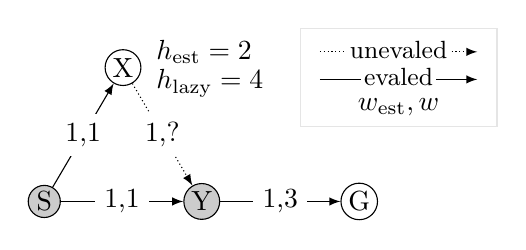
\begin{tikzpicture}
      \tikzset{>=latex} % arrow heads
      %\draw[step=1cm,black!10,very thin] (0,0) grid (8,4);
      \node[draw,circle,inner sep=1pt,fill=black!20] (S) at (1,1) {S};
      \node[draw,circle,inner sep=1pt] (X) at (2,2.7) {X};
      \node[draw,circle,inner sep=1pt,fill=black!20] (Y) at (3,1) {Y};
      \node[draw,circle,inner sep=1pt] (G) at (5,1) {G};
      \draw[->] (S) -- (Y) node [midway,fill=white] {1,1};
      \draw[->] (Y) -- (G) node [midway,fill=white] {1,3};
      \draw[->] (S) -- (X) node [midway,fill=white] {1,1};
      \draw[->,densely dotted] (X) -- (Y) node [midway,fill=white] {1,?};
      \node[anchor=west] at (2.3,2.9) {$h_{\ms{est}} = 2$};
      \node[anchor=west] at (2.3,2.5) {$h_{\ms{lazy}} = 4$};
      
      % for legend
      %\node at (7,2.9) {unevaluated:};
      %\draw[->,dashed] (6,2.5) -- (8,2.5)
      %   node [midway,fill=white] {($w_{est}$)\,?};
      %\node at (7,1.9) {evaluated:};
      %\draw[->] (6,1.5) -- (8,1.5)
      %   node [midway,fill=white] {($w_{est}$)\,$w$};
      \draw[->,densely dotted] (4.5,2.9) -- (6.5,2.9)
         node[midway,yshift=0.03cm,fill=white,inner sep=1pt,font=\small] {unevaled};
      \draw[->] (4.5,2.55) -- (6.5,2.55)
         node[midway,yshift=0.03cm,fill=white,inner sep=1pt,font=\small] {evaled};
      \node at (5.5,2.2) {$w_{\ms{est}},w$};
      \draw[black!10] (4.25,1.95) rectangle (6.75,3.2);
   \end{tikzpicture}
   \caption{A* comparison between
      the static goal heuristic $h_{\ms{est}}$ (\ref{eqn:h_est})
      and the dynamic goal heuristic $h_{\ms{lazy}}$ (\ref{eqn:h_lazy})
      on a simple graph from start S to goal G.
      The values of both the edge weight estimate $w_{\ms{est}}$
      and the true edge weight $w$ (for evaluated edges) are shown.
      Using either goal heuristic,
      the A* algorithm first expands vertices S and Y,
      evaluating three edges in total and leaving X and G on OPEN.
      After finding that edge YG has $w=3$,
      the dynamic heuristic value $h_{\ms{lazy}}(\mbox{X})$
      is updated from 2 to 4.
      While the A* using the static $h_{\ms{est}}$ would next expand X,
      the A* using the dynamic $h_{\ms{lazy}}$ would next expand G
      and terminate, having never evaluated edge XY.}
   \label{fig:updating-heuristic}
\end{figure}

\textbf{A* with a dynamic heuristic.}
In order to apply A* and Lazy Weighted A* to our problem,
we need a goal heuristic over vertices.
The most simple may be
\begin{equation}
   h_{\ms{est}}(v) = \min_{p : v \rightarrow v_g} \mbox{len}(p, w_{\ms{est}}).
   \label{eqn:h_est}
\end{equation}
Note that the value of this heuristic could be computed as a
pre-processing step using Dijkstra's algorithm \citep{dijkstra1959anote}
before iterations begin.
However,
in order for the equivalences to hold,
we require the use of the lazy heuristic
\begin{equation}
   h_{\ms{lazy}}(v) = \min_{p : v \rightarrow v_g} \mbox{len}(p, w_{\ms{lazy}}).
   \label{eqn:h_lazy}
\end{equation}
This heuristic is dynamic in that it depends on $w_{\ms{lazy}}$
which changes as edges are evaluated.
Therefore,
heuristic values must be recomputed for all affected vertices on OPEN
after each iteration.
%An illustrative example is shown in
%Figure~\ref{fig:updating-heuristic}.
%(We discuss efficient implementation of $h_{\ms{lazy}}$ as it relates
%to the D* family of algorithms in Section~\ref{sec:discussion}.)

\subsection{Equivalence to A*}

We show that the LazySP-Expand algorithm
is edge-equivalent to a variant of the A*
shortest-path algorithm.
%We consider the variant of A* which allows a vertex $v$ to be reopened
%if its stored cost $g[v]$ is improved.
We make use of two invariants that are maintained during the
progression of A*.
Proofs are provided in the appendix.
\begin{invariant}
If $v$ is discovered by A* and $v'$ is undiscovered,
with $v'$ a successor of $v$,
then $v$ is on OPEN.%
\label{inv:astar-cundisc-popen}%
\end{invariant}
\begin{invariant}
If $v$ and $v'$ are discovered by A*,
with $v'$ a successor of $v$,
and $g[v] + w(v,v') < g[v']$,
then $v$ is on OPEN.%
\label{inv:astar-wless-popen}%
\end{invariant}
When we say a vertex is \emph{discovered},
we mean that it is either on OPEN or CLOSED.
Note that Invariant \ref{inv:astar-wless-popen} holds
because we allow vertices to be reopened;
without reopening (and with an inconsistent heuristic),
later finding a cheaper path to $v$ (and not reopening $v'$)
would invalidate the invariant.

We will use the goal heuristic $h_{\ms{lazy}}$ from (\ref{eqn:h_lazy}).
Note that if an admissible edge weight estimator $\hat{w}$ exists
(that is, $\hat{w} \leq w$),
then our A* can approximate the Weighted A* algorithm
\citep{pohl1970weightedastar}
with parameter $\epsilon$
by using $w_{\ms{est}} = \epsilon \, \hat{w}$,
and the suboptimality bound from
Theorem~\ref{thm:lazy-optimality} holds.

\begin{figure}[t]
   \centering
   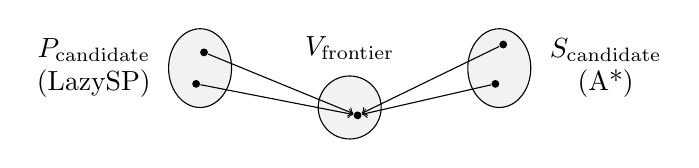
\begin{tikzpicture}
      %\draw[step=1cm,gray,very thin] (0,0) grid (8,3);
      
      \draw[fill=black!05] (2.1,1.5) ellipse (0.4cm and 0.5cm);
      \draw[fill=black!05] (5.9,1.5) ellipse (0.4cm and 0.5cm);
      \draw[fill=black!05] (4,1) ellipse (0.4cm and 0.4cm);
      
      \node[align=center] at (0.75,1.5) {$P_{\ms{candidate}}$\\(LazySP)};
      \node[align=center] at (7.25,1.5) {$S_{\ms{candidate}}$\\(A*)};
      \node[align=center] at (4,1.75) {$V_{\ms{frontier}}$};
      
      \node[fill=black,circle,inner sep=1pt] (p1) at (2.15,1.7) {};
      \node[fill=black,circle,inner sep=1pt] (p2) at (2.05,1.3) {};
      
      \node[fill=black,circle,inner sep=1pt] (s1) at (5.95,1.8) {};
      \node[fill=black,circle,inner sep=1pt] (s2) at (5.85,1.3) {};
      
      \node[fill=black,circle,inner sep=1pt] (v1) at (4.1,0.9) {};
      
      \draw[->] (p1) -- (v1);
      \draw[->] (p2) -- (v1);
      
      \draw[->] (s1) -- (v1);
      \draw[->] (s2) -- (v1);
      
   \end{tikzpicture}
   \caption{Illustration of the equivalence
      between A* and LazySP-Expand.
      After evaluating the same set of edges,
      the next edges to be evaluated by each algorithm
      can both be expressed as a surjective mapping onto
      a common set of unexpanded
      frontier vertices.
      }
   \label{fig:astar-equiv-mapping}
\end{figure}

\textbf{Equivalence.}
In order to show edge-equivalence,
we consider the case where both algorithms
are beginning a new iteration
having so far evaluated the same set of edges.

LazySP-Expand has some set $P_{\ms{candidate}}$ of allowable
candidate paths minimizing $\mbox{len}(p,w_{\ms{lazy}})$;
the Expand selector will then identify a vertex on the chosen path
for expansion.

A* will iteratively select a set of vertices from OPEN to expand.
Because it is possible that a vertex is expanded multiple times
(and only the first expansion results in edge evaluations),
we group iterations of A* into \emph{sequences},
where each sequence $s$ consists of
(a) zero or more vertices from OPEN that have already been expanded,
followed by (b) one vertex from OPEN that is to be expanded
for the first time.

We show that both the set of allowable candidate paths $P_{\ms{candidate}}$
available to LazySP-Expand
and the set of allowable candidate vertex sequences $S_{\ms{candidate}}$
available to A*
map surjectively to the same set of unexpanded frontier vertices $V_{\ms{frontier}}$
as illustrated in Figure~\ref{fig:astar-equiv-mapping}.
This is described by way of
Theorems \ref{thm:astar-equiv-from-lazy}
and \ref{thm:astar-equiv-to-lazy} below
(proofs in appendix).

\begin{theorem}
If LazySP-Expand and A* have evaluated the same set of edges,
then for any candidate path $p_{\ms{candidate}}$ chosen by LazySP
yielding frontier vertex $v_{\ms{frontier}}$,
there exists an allowable A* sequence $s_{\ms{candidate}}$
which also yields $v_{\ms{frontier}}$.
\label{thm:astar-equiv-from-lazy}
\end{theorem}

\begin{theorem}
If LazySP-Expand and A* have evaluated the same set of edges,
then for any candidate sequence $s_{\ms{candidate}}$ chosen by A*
yielding frontier vertex $v_{\ms{frontier}}$,
there exists an allowable LazySP path $p_{\ms{candidate}}$
which also yields $v_{\ms{frontier}}$.
\label{thm:astar-equiv-to-lazy}
\end{theorem}

\subsection{Equivalence to Lazy Weighted A*}

%\begin{algorithm}
%   \caption{Forward Edge Evaluation Selector}
%   \begin{algorithmic}[1]
%   \Function {\textsc{SelectForward}}{$G, p_{\ms{candidate}}$}
%   \State $e_{\ms{first}} \leftarrow$ first unevaluated $e \in p_{\ms{candidate}}$
%   \State \Return $\{ e_{\ms{first}} \}$
%   \EndFunction
%   \end{algorithmic}
%   \label{alg:selectforward}
%\end{algorithm}

In a conventional vertex expansion algorithm,
determining a successor's cost is a function of both
the cost of the edge and the value of the heuristic.
If either of these components is expensive to evaluate,
an algorithm can defer its computation by maintaining the successor
on the frontier with an approximate cost until it is expanded.
The Fast Downward algorithm \citep{helmert2006fastdownward} is motivated
by expensive heuristic evaluations in planning,
whereas the Lazy Weighted A* (LWA*) algorithm \citep{cohen2014narms}
is motivated by expensive edge evaluations in robotics.

We show that the LazySP-Forward algorithm
is edge-equivalent to a variant of the Lazy Weighted A*
shortest-path algorithm.
For a given candidate path,
the Forward selector returns the first unevaluated edge.

\textbf{Variant of Lazy Weighted A*.}
We reproduce a variant of LWA* without a CLOSED list
in Algorithm~\ref{alg:lwastar}.
For the purposes of our analysis,
the reproduction differs from the original presentation,
and we detail those differences here.
With the exception of the lack of CLOSED,
the differences do not affect the behavior of the algorithm.

\begin{algorithm}[t]
\caption{Lazy Weighted A* (without CLOSED list)}
\label{alg:lwastar}
\begin{algorithmic}[1]
\Function {\textsc{LazyWeightedA*}}{$G, w, \hat{w}, h$}
\State $g[v_{\ms{start}}] \leftarrow 0$
\State $Q_v \leftarrow \{ v_{\ms{start}} \}$
   \Comment Key: $g[v] + h(v)$
   \label{line:lwastar-key-qvertices}
\State $Q_e \leftarrow \emptyset$
   \Comment Key: $g[v] + \hat{w}(v,v') + h(v')$
   \label{line:lwastar-key-qedges}
\While {$\min(Q_v.{\mbox{TopKey}}, Q_e.{\mbox{TopKey}}) < g[v_{\ms{goal}}]$}
   \If {$Q_v.{\mbox{TopKey}} \leq Q_e.{\mbox{TopKey}}$}
      \State $v \leftarrow Q_v.{\mbox{Pop}}()$
      \For {$v' \in G.\mbox{GetSuccessors}(v)$}
         \State $Q_e.\mbox{Insert}((v,v'))$
      \EndFor
   \Else
      \State $(v,v') \leftarrow Q_e.{\mbox{Pop}}()$
      \If {$g[v'] \leq g[v] + \hat{w}(v,v')$}
         \label{line:lwastar-test}
         \State {\bf continue}
      \EndIf
      \State $g_{\ms{new}} \leftarrow g[v] + w(v,v')$
         \Comment evaluate
      \If {$g_{\ms{new}} < g[v']$}
         \State $g[v'] = g_{\ms{new}}$
         \State $Q_v.\mbox{Insert}(v')$
      \EndIf
   \EndIf
\EndWhile
\EndFunction
\end{algorithmic}
\end{algorithm}

The most obvious difference is that we present the original OPEN list
as separate vertex ($Q_v$) and edge ($Q_e$) priority queues,
with sorting keys shown on lines \ref{line:lwastar-key-qvertices}
and \ref{line:lwastar-key-qedges}.
A vertex $v$ in the original OPEN with $trueCost(v) = true$
corresponds to a vertex $v$ in $Q_v$,
whereas a vertex $v'$ in the original OPEN
with $trueCost(v') = false$ (and parent $v$)
corresponds to an edge $(v,v')$ in $Q_e$.
Use of the edge queue obviates the need for
duplicate vertices on OPEN with different parents
and the $conf(v)$ test for identifying such duplicates.
This presentation also highlights the similarity between LWA*
and the inner loop of the Batch Informed Trees (BIT*) algorithm
\citep{gammell2015bitstar}.

The second difference is that the edge usefulness test
(line 12 of the original algorithm)
has been moved from before inserting into OPEN
to after being popped from OPEN,
but before being evaluated
(line~\ref{line:lwastar-test} of Algorithm~\ref{alg:lwastar}).
This change is partially in compensation for removing the CLOSED
list.
This adjustment
does not affect the edges evaluated.

We make use of an invariant that is maintained during the
progression of Lazy Weighted A* (proof in appendix).
\begin{invariant}
For all vertex pairs $v$ and $v'$,
with $v'$ a successor of $v$,
if $g[v] + \max(w(v,v'), \hat{w}(v,v')) < g[v']$,
then either vertex $v$ is on $Q_{v}$
or edge $(v,v')$ is on $Q_e$.%
\label{inv:lwastar}%
\end{invariant}
We will use $h(v) = h_{\ms{lazy}}(v)$ from (\ref{eqn:h_lazy})
and $\hat{w} = w_{\ms{lazy}}$.
Note that the use of these dynamic heuristics requires that the
$Q_v$ and $Q_e$ be resorted after every edge is evaluated.

\textbf{Equivalence.}
The equivalence follows similarly to that for A* above.
Given the same set of edges evaluated,
the set of allowable next evaluations is identical for each
algorithm.

\begin{theorem}
If LazySP-Forward and LWA* have evaluated the same set of edges,
then for any allowable candidate path $p_{\ms{candidate}}$
chosen by LazySP yielding first unevaluated edge $e_{ab}$,
there exists an allowable LWA* sequence $s_{\ms{candidate}}$
which also yields $e_{ab}$.
\label{thm:lwastar-equiv-from-lazy}
\end{theorem}

\begin{theorem}
If LazySP-Forward and LWA* have evaluated the same set of edges,
then for any allowable sequence of vertices and edges $s_{\ms{candidate}}$
considered by LWA* yielding evaluated edge $e_{ab}$,
there exists an allowable LazySP candidate path $p_{\ms{candidate}}$
which also yields $e_{ab}$.
\label{thm:lwastar-equiv-to-lazy}
\end{theorem}

\subsection{Relation to Bidirectional Heuristic Search}

LazySP-Alternate chooses unevaluated edges from either
the beginning or the end of the candidate path at each iteration.
We conjecture that an alternating version of the Expand selector
is edge-equivalent to the
Bidirectional Heuristic Front-to-Front Algorithm
\citep{champeauxsint1977bhffa}
for appropriate lazy vertex pair heuristic,
and that LazySP-Alternate is edge-equivalent
to a bidirectional LWA*.

\begin{algorithm}[t]
   \caption{Maximum Edge Probability Selector
      \emph{(for WeightSamp and Partition path distributions)}}
   \begin{algorithmic}[1]
   \Function {\textsc{SelectMaxEdgeProb}}{$G, p_{\ms{candidate}}, \mathcal{D}_p$}
   \State $p(e) \leftarrow \Pr( \, e \in P \, )
      \mbox{ for } P \sim \mathcal{D}_p$
   \State $e_{\ms{max}} \leftarrow$ unevaluated $e \in p_{\ms{candidate}}$
      maximizing $p(e)$
   \State \Return $\{ e_{\ms{max}} \}$
   \EndFunction
   \end{algorithmic}
   \label{alg:selectmaxscore}
\end{algorithm}

\section{Novel Edge Selectors}

Because we are conducting a search over paths,
we are free to implement selectors which are not constrained to
evaluate edges in any particular order
(i.e. to maintain evaluated trees rooted at the start and goal
vertices).
In this section,
we describe a novel class of edge selectors which is designed
to reduce the total number of edges evaluated during the course
of the LazySP algorithm.
These selectors operate by maintaining a distribution over potential
paths at each iteration of the algorithm
(see Figure~\ref{fig:maxprob-selectors-overview}).
This path distribution induces a Bernoulli distribution for each
edge $e$ which indicates its probability $p(e)$ to lie on
the potential path;
at each iteration,
the selectors then choose the unevaluated edge that maximizes
this edge indicator probability (Algorithm~\ref{alg:selectmaxscore}).
The two selectors described in this section differ
with respect to how they maintain this distribution over potential paths.

% make -f e8_experiments/scripts/Makefile.lazysp-fig-dists
\begin{figure}[t]
   \centering
   \begin{tikzpicture}
      \tikzset{>=latex}
      
      \node[draw,minimum width=2.4cm,minimum height=3.0cm] (startbox) at (-3.0,0) {};
      \node[inner sep=0pt] at (-3.0,-0.35) {\includegraphics[scale=2.0]{build/lazysp-fig-dists/fig-sofar}};
      \node[align=center,font=\small,below] at (startbox.north) {known\\edges};
      
      \node[draw] (quesbox) at (-1.2,0) {?};
      
      \node[draw,minimum width=2.1cm,minimum height=3.0cm] (pathsbox) at (0.4,0) {};
      \node[inner sep=0pt] at (-0.05, 0.1) {\includegraphics[scale=0.8]{build/lazysp-fig-dists/fig-path-00}};
      \node[inner sep=0pt] at ( 0.85, 0.1) {\includegraphics[scale=0.8]{build/lazysp-fig-dists/fig-path-01}};
      \node[inner sep=0pt] at (-0.05,-0.8) {\includegraphics[scale=0.8]{build/lazysp-fig-dists/fig-path-02}};
      \node[inner sep=0pt] at ( 0.85,-0.8) {\includegraphics[scale=0.8]{build/lazysp-fig-dists/fig-path-03}};
      \node[align=center,font=\small,below] at (pathsbox.north) {path\\distribution};
      \node[align=center,font=\normalsize,above] at (pathsbox.south) {$\dots$};
      
      \node[draw,minimum width=2.4cm,minimum height=3.0cm] (goalbox) at (3.0,0) {};
      \node[inner sep=0pt] at (3.0,-0.35) {\includegraphics[scale=2.0]{build/lazysp-fig-dists/fig-dist-probs}};
      \node[align=center,font=\small,below] at (goalbox.north) {edge indicator\\distributions};
      
      \draw[->] (startbox) -- (quesbox);
      \draw[->] (quesbox) -- (pathsbox);
      \draw[->] (pathsbox) -- (goalbox);
      
   \end{tikzpicture}
   \caption{Illustration of maximum edge probability selectors.
      A distribution over paths
      (usually conditioned on the known edge evaluations)
      induces on each edge $e$ a Bernoulli distribution
      with parameter $p(e)$
      giving the probability that it belongs to the path.
      The selector chooses the edge with the largest such probability.}
   \label{fig:maxprob-selectors-overview}
\end{figure}

\subsection{Weight Function Sampling Selector}

The first selector, WeightSamp,
is motivated by the intuition that it is preferable to evaluate edges
that are most likely to lie on the true shortest path.
Therefore,
it computes its path distribution $\mathcal{D}_p$
by performing shortest path queries
on sampled edge weight functions drawn from a distribution
$\mathcal{D}_w$.
This edge weight distribution is conditioned on the the known weights
of all previously evaluated edges $E_{\ms{eval}}$:
\begin{equation}
   \mathcal{D}_p : \mbox{SP}(w)
   \mbox{ for } w \sim \mathcal{D}_w(E_{\ms{eval}})
   \label{eqn:weightsamp}.
\end{equation}

For example,
the distribution $\mathcal{D}_w$ might consist of
the edge weights induced by a model of the distribution of
environment obstacles
(Figure~\ref{fig:weightsamp}).
Since this obstacle distribution is conditioned on the results
of known edge evaluations,
we consider the subset of worlds which are consistent
with the edges we have evaluated so far.
However,
depending on the fidelity of this model,
solving the corresponding shortest path problem for a given
sampled obstacle arrangement might require as much computation as
solving the original problem,
since it requires computing the resulting edge weights.
In practice,
we can approximate $\mathcal{D}_w$
by assuming that each edge is independently distributed.

\begin{figure}[t]
   \centering
   \begin{tikzpicture}
      \tikzset{>=latex}
      
      \node[draw,minimum width=1.8cm,minimum height=2.6cm] (startbox) at (-4.4,0) {};
      \node[inner sep=0pt] at (-4.4,-0.35) {\includegraphics[scale=1.5]{build/lazysp-fig-dists/fig-sofar}};
      \node[align=center,font=\small,below] at (startbox.north) {known\\edges};
      
      \node[draw,minimum width=1.8cm,minimum height=6cm] (abox) at (-2.2,0) {};
      \node[inner sep=0pt] at (-2.2, 1.3) {\includegraphics[scale=1.5]{build/lazysp-fig-dists/fig-world-00}};
      \node[inner sep=0pt] at (-2.2,-0.3) {\includegraphics[scale=1.5]{build/lazysp-fig-dists/fig-world-01}};
      \node[inner sep=0pt] at (-2.2,-1.9) {\includegraphics[scale=1.5]{build/lazysp-fig-dists/fig-world-02}};
      \node[align=center,font=\small,below] at (abox.north) {obstacle\\distribution};
      \node[align=center,font=\normalsize,above] at (abox.south) {$\dots$};
      
      \node[draw,minimum width=1.8cm,minimum height=6cm] (bbox) at (0,0) {};
      \node[inner sep=0pt] at (0, 1.3) {\includegraphics[scale=1.5]{build/lazysp-fig-dists/fig-wfn-00}};
      \node[inner sep=0pt] at (0,-0.3) {\includegraphics[scale=1.5]{build/lazysp-fig-dists/fig-wfn-01}};
      \node[inner sep=0pt] at (0,-1.9) {\includegraphics[scale=1.5]{build/lazysp-fig-dists/fig-wfn-02}};
      \node[align=center,font=\small,below] at (bbox.north) {weight fn\\distribution};
      \node[align=center,font=\normalsize,above] at (bbox.south) {$\dots$};
      
      \node[draw,minimum width=1.8cm,minimum height=6cm] (cbox) at (2.2,0) {};
      \node[inner sep=0pt] at (2.2, 1.3) {\includegraphics[scale=1.5]{build/lazysp-fig-dists/fig-path-00}};
      \node[inner sep=0pt] at (2.2,-0.3) {\includegraphics[scale=1.5]{build/lazysp-fig-dists/fig-path-01}};
      \node[inner sep=0pt] at (2.2,-1.9) {\includegraphics[scale=1.5]{build/lazysp-fig-dists/fig-path-02}};
      \node[align=center,font=\small,below] at (cbox.north) {path\\distribution};
      \node[align=center,font=\normalsize,above] at (cbox.south) {$\dots$};
      
      \draw[->] (startbox) -- (abox);
      \draw[->] (abox) -- (bbox);
      \draw[->] (bbox) -- (cbox);
   \end{tikzpicture}
   \caption{The WeightSamp selector uses the path distribution induced by
      solving the shortest path problem on a distribution over possible
      edge weight functions $\mathcal{D}_w$.
      In this example, samples from $\mathcal{D}_w$ are computed by
      drawing samples from $\mathcal{D}_O$,
      the distribution of obstacles that are consistent with
      the known edge evaluations.}
   \label{fig:weightsamp}
\end{figure}

\subsection{Partition Function Selector}

While the WeightSamp selector captures the intuition that it is
preferable to focus edge evaluations in areas that are useful for
many potential paths,
the computational cost required to calculate it at each iteration
may render it intractable.
One candidate path distribution that is more efficient to compute
follows an exponential form:
\begin{equation}
   \mathcal{D}_p : f_P(p) \propto
   \exp( - \beta \, \mbox{len}(p, w_{\ms{lazy}}) ).
\end{equation}
In other words,
we consider all potential paths $P$
between the start and goal vertices,
with shorter paths assigned more probability than longer ones
(with positive parameter $\beta$).
We call this the Partition selector
because this distribution is closely related to calculating
partition functions from statistical mechanics.
The corresponding partition function is:
\begin{equation}
   Z(P) = \sum_{p \in P}
      \exp( - \beta \, \mbox{len}(p, w_{\ms{lazy}}) ).
   \label{eqn:partitionfn}
\end{equation}
Note that the edge indicator probability
required in Algorithm~\ref{alg:selectmaxscore}
can then be written:
\begin{equation}
   p(e) = 1 - \frac{Z(P \setminus e)}{Z(P)}.
   \label{eqn:edge-ind-prob}
\end{equation}
Here, $P \setminus e$ denotes paths in $P$ that do not
contain edge $e$.

\begin{figure}
   \centering
   \subfloat[Initial $p(e)$ scores on a constant-weight
         grid with $\beta$: 50, 33, 28]{%
      \centering
      \includegraphics{build/lazysp-selscores/empty-50}
      \includegraphics{build/lazysp-selscores/empty-33}
      \includegraphics{build/lazysp-selscores/empty-28}
      \label{subfig:partition-empty}
   }
   
   \subfloat[Initial $p(e)$ scores with $\infty$-weight
         obstacles with $\beta$: 50, 33, 28]{%
      \centering
      \includegraphics{build/lazysp-selscores/gap-50}
      \includegraphics{build/lazysp-selscores/gap-33}
      \includegraphics{build/lazysp-selscores/gap-28}
      \label{subfig:partition-passage}
   }
   
   % $ rosrun e8_experiments lazysp-partall-figure.py
   % --probdir=prob-box2d08-halton-roots12
   % --snapshot-afteredges=0 --out-tikz=partall-figure-0.tex
   \subfloat[Initial $p(e)$ scores]{%
      \centering
      \includegraphics{build/lazysp-partall/partall-figure-0}
      \label{subfig:partition-example-initial}
   }
   % $ rosrun e8_experiments lazysp-partall-figure.py
   % --probdir=prob-box2d08-halton-roots12
   % --snapshot-afteredges=5 --out-tikz=partall-figure-5.tex
   \subfloat[Scores after five evaluations]{%
      \centering
      \includegraphics{build/lazysp-partall/partall-figure-5}
      \label{subfig:partition-example-after5}
   }

   \caption{Examples of the Partition selector's
      $p(e)$ edge score function.
      %(\subref{subfig:partition-empty})
      With no known obstacles,
      a high $\beta$ assigns near-unity score to only edges on the
      shortest path;
      as $\beta$ decreases and more paths are considered,
      edges immediately adjacent to the roots score highest.
      %(\subref{subfig:partition-passage})
      Since all paths must pass
      through the narrow passage,
      edges within score highly.
      %(\subref{subfig:partition-example-initial})
      For a problem with two a-priori known obstacles (dark gray),
      the score first prioritizes evaluations between the two.
      %(\subref{subfig:partition-example-after5})
      Upon finding these edges are blocked,
      the next edges that are prioritized lie along the top of the world.}
   \label{ref:example-scores}
\end{figure}

It may appear advantageous to restrict $P$ to only
\emph{simple} paths,
since all optimal paths are simple.
Unfortunately,
an algorithm for computing (\ref{eqn:edge-ind-prob}) efficiently is not
currently known in this case.
However,
in the case that $P$ consists of all paths,
there exists an efficient incremental calculation of
(\ref{eqn:partitionfn}) via a recursive formulation
which we detail here.

We use the notation $Z_{xy} = Z(P_{xy})$,
with $P_{xy}$ the set of paths from $x$ to $y$.
Suppose the values $Z_{xy}$ are known between
all pairs of vertices $x, y$ for a graph $G$.
(For a graph with no edges,
$Z_{xy}$ is 1 if $x = y$ and 0 otherwise.)
Consider a modified graph $G'$ with one additional edge $e_{ab}$
with weight $w_{ab}$.
All additional paths use the new edge $e_{ab}$ a non-zero
number of times;
the value $Z'_{xy}$ can be shown to be
\begin{equation}
   Z'_{xy} = Z_{xy} + \frac{Z_{xa} Z_{by}}{\exp(\beta w_{ab}) - Z_{ba}}
   \mbox{ if }
   \exp(\beta w_{ab}) > Z_{ba}.
\end{equation}
This form is derived from simplifying the induced geometric series;
note that if $\exp(\beta w_{ab})  \leq Z_{ba}$,
the value $Z'_{xy}$ is infinite.
One can also derive the inverse:
given values $Z'$,
calculate the values $Z$ if an edge were removed.
A derivation of this formulation is given in
Appendix~\ref{chap:appendix-partition}.

This incremental formulation of (\ref{eqn:partitionfn})
allows for the corresponding score $p(e)$ for edges
to be updated efficiently during each iteration of LazySP as
the $w_{\ms{lazy}}$ value for edges chosen for evaluation are updated.
In fact,
if the values $Z$ are stored in a square matrix,
the update for all pairs after an edge weight change consists of a single
vector outer product.

\section{Experiments}

We compared the seven edge selectors on three classes of shortest path
problems.
The average number of edges evaluated by each,
as well as timing results from our implementations,
are shown in Figure~\ref{fig:results}.
In each case,
the estimate was chosen so that $w_{\ms{est}} \leq w$,
so that all runs produced optimal paths.
The experimental results serve primarily to illustrate that
the A* and LWA* algorithms
(i.e. Expand and Forward)
are not optimally edge-efficient,
but they also expose differences in behavior and prompt
future research directions.
All experiments were conducted using an open-source
implementation.
Motion planning results were implemented using
OMPL \citep{sucan2012ompl}.

\textbf{Random partially-connected graphs.}
We tested on a set of 1000 randomly-generated undirected graphs
with $|V|=100$,
with each pair of vertices sharing an edge with probability 0.05.
Edges have an independent 0.5 probability of having infinite weight,
else the weight is uniformly distributed on $[1,2]$;
the estimated weight was unity for all edges.
For the WeightSamp selector,
we drew 1000 $w$ samples.
For the Partition selector, we used $\beta = 2$.

\textbf{Roadmap graphs on the unit square.}
We considered roadmap graphs formed via the first 100 points
of the $(2,3)$-Halton sequence on the unit square
with a connection radius of 0.15,
with 30 pairs of start and goal vertices chosen randomly.
The edge weight function was derived from 30 sampled obstacle fields
consisting of 10 randomly placed boxes
with dimensions uniform on $[0.1,0.3]$,
with each edge having infinite weight on collision,
and weight equal to its Euclidean length otherwise.
One of the resulting 900 example problems is shown in
Figure~\ref{fig:snapshots}.
For the WeightSamp selector,
we drew 1000 $w$ samples
with a na\"{\i}ve edge weight distribution in which
each edge had an independent 0.1 collision probability.
For the Partition selector, we used $\beta = 21$.

\textbf{Roadmap graphs for robot arm motion planning.}
We considered roadmap graphs in the configuration space
corresponding to 7-DOF right arm of the HERB home robot across three
motion planning problems inspired by a table clearing scenario
(see Figure~\ref{fig:herbbin0}).
The problems consisted of first moving from the robot's
home configuration to one of 7 feasible grasp configurations for a mug
(pictured),
second transferring the mug to one of 72 feasible configurations with
the mug above the blue bin,
and third returning to the home configuration.
Each problem was solved independently.
This common scenario spans various numbers of starts/goals
and allows a comparison w.r.t. difficulty at different problem
stages as discussed later.

For each problem,
50 random graphs were constructed by applying a random offset to
the 7D Halton sequence with $N = 1000$,
with additional vertices for each problem start and goal configuration.
We used an edge connection radius of 3 rad,
resulting $|E|$ ranging from 23404 to 28109.
Each edge took infinite weight on collision,
and weight equal to its Euclidean length otherwise.
For the WeightSamp selector,
we drew 1000 $w$ samples
with a na\"{\i}ve edge weight distribution in which
each edge had an independent 0.1 probability of collision.
For the Partition selector, we used $\beta = 3$.

\begin{figure*}
\centering
%\includegraphics[width=3cm]{figs/herbbin0.png}
\includegraphics[width=3.1cm]{figs/lazysp-herbarm/herbarm-roadmap.png}
\includegraphics[width=3.1cm]{figs/lazysp-herbarm/herbarm-path02.png}
%\includegraphics[width=3cm]{figs/lazysp-herbarm/herbarm-path11.png}
%\includegraphics[width=3cm]{figs/lazysp-herbarm/herbarm-path21.png}
\includegraphics[width=3.1cm]{figs/lazysp-herbarm/herbarm-path33.png}
\includegraphics[width=3.1cm]{figs/lazysp-herbarm/herbarm-path42.png}
\includegraphics[width=3.1cm]{figs/lazysp-herbarm/herbarm-path46.png}
\caption{Visualization of the first of three articulated motion
   planning problems in which the HERB robot must move its right arm
   from the start configuration (pictured)
   to any of seven grasp configurations for a mug.
   Shown is the progression of the Alternate selector on one of the
   randomly generated roadmaps;
   approximately 2\% of the 7D roadmap is shown in gray by projecting
   onto the space of end-effector positions.}
\label{fig:herbbin0}
\end{figure*}

\begin{figure}[t!]
   \centering
   \subfloat[
      Average number of edges evaluated for each problem class
         and selector.
         The minimum selector,
         along with any selector within one unit of its standard error,
         is shown in bold.
         The ArmPlan class is split into its three constituent problems.
         Online timing results are also shown,
         including the components from the invoking the selector
         and evaluating edges.
         \dag PartConn and UnitSquare involve trivial edge evaluation
         time.
         \ddag Timing for the Partition selector does not include
         pre-computation time.
         See Figure~\ref{fig:table-timing-results} for details.]
   {%
      \centering
      {\small%
      \setlength{\tabcolsep}{0.06cm}%
      \begin{tabular}{lrrrrrrr}
         \toprule
            & E\;\;\;\;
            & F\;\;\;\; & R\;\;\;\; & A\;\;\;\;
            & B\;\;\;\; & W\;\;\;\; & P\ddag\;\; \\
         \midrule
         \addlinespace[0.3em]
         PartConn &  87.10 & 35.86 & 34.84 & 22.23 & 44.81 & \textbf{20.66} & \textbf{20.39} \\
         \;\;\emph{online\dag (ms)} & \bf\emph{1.22} & \emph{1.96} & \emph{1.86} & \bf\emph{1.20} & \emph{2.41} & \emph{4807.19} & \emph{3.32} \\
         \;\;\;\;\emph{sel (ms)} & \emph{0.02} & \emph{0.01} & \emph{0.01} & \emph{0.01} & \emph{0.03} & \emph{4805.64} & \emph{2.07} \\
         \addlinespace[0.3em]
         UnitSquare &  69.21 & 27.29 & 27.69 & 17.82 & 32.62 & 15.58 & \textbf{14.08} \\
         \;\;\emph{online\dag (ms)} & \bf\emph{0.91} & \emph{1.47} & \emph{1.49} & \bf\emph{0.94} & \emph{1.71} & \emph{3864.95} & \emph{1.72} \\
         \;\;\;\;\emph{sel (ms)} & \emph{0.01} & \emph{0.01} & \emph{0.01} & \emph{0.01} & \emph{0.02} & \emph{3863.49} & \emph{0.87} \\
         \addlinespace[0.3em]
         ArmPlan(avg) & 949.05 & 63.62 & 74.94 & 55.48 & 68.01 & 56.93 & \textbf{48.07} \\
         \;\;\emph{online (s)} & \emph{269.82} & \bf\emph{5.90} & \emph{8.22} & \bf\emph{5.96} & \emph{7.34} & \emph{3402.21} & \bf\emph{5.80} \\
         \;\;\;\;\emph{sel (s)} & \emph{0.00} & \emph{0.00} & \emph{0.00} & \emph{0.00} & \emph{0.00} & \emph{3392.76} & \emph{1.54} \\
         \;\;\;\;\emph{eval (s)} & \emph{269.78} & \emph{5.87} & \emph{8.20} & \emph{5.94} & \emph{7.31} & \emph{9.39} & \emph{4.21} \\
         \addlinespace[0.3em]
         ArmPlan1 &  344.74 & \textbf{49.72} & 95.58 & 59.44 & 58.90 & 73.72 & \textbf{50.66} \\
         \;\;\emph{online (s)} & \emph{109.09} & \bf\emph{4.81} & \emph{14.81} & \emph{7.03} & \emph{7.91} & \emph{3375.35} & \emph{7.25} \\
         \;\;\;\;\emph{sel (s)} & \emph{0.00} & \emph{0.00} & \emph{0.00} & \emph{0.00} & \emph{0.00} & \emph{3358.82} & \emph{1.61} \\
         \;\;\;\;\emph{eval (s)} & \emph{109.07} & \emph{4.78} & \emph{14.77} & \emph{7.01} & \emph{7.88} & \emph{16.47} & \emph{5.59} \\
         \addlinespace[0.3em]
         ArmPlan2 &  657.02 & \textbf{62.24} & 98.54 & 69.96 & 75.88 & \textbf{66.24} & \textbf{62.16} \\
         \;\;\emph{online (s)} & \emph{166.19} & \bf\emph{3.27} & \emph{7.36} & \emph{5.95} & \emph{5.63} & \emph{4758.04} & \emph{5.99} \\
         \;\;\;\;\emph{sel (s)} & \emph{0.00} & \emph{0.00} & \emph{0.00} & \emph{0.00} & \emph{0.00} & \emph{4750.16} & \emph{2.03} \\
         \;\;\;\;\emph{eval (s)} & \emph{166.17} & \emph{3.26} & \emph{7.34} & \emph{5.93} & \emph{5.61} & \emph{7.82} & \emph{3.91} \\
         \addlinespace[0.3em]
         ArmPlan3 & 1845.38 & 78.90 & \textbf{30.70} & 37.04 & 69.26 & \textbf{30.82} & \textbf{31.38} \\
         \;\;\emph{online (s)} & \emph{534.16} & \emph{9.61} & \bf\emph{2.50} & \emph{4.91} & \emph{8.47} & \emph{2073.23} & \emph{4.17} \\
         \;\;\;\;\emph{sel (s)} & \emph{0.00} & \emph{0.00} & \emph{0.00} & \emph{0.00} & \emph{0.00} & \emph{2069.29} & \emph{0.98} \\
         \;\;\;\;\emph{eval (s)} & \emph{534.10} & \emph{9.58} & \emph{2.48} & \emph{4.89} & \emph{8.44} & \emph{3.90} & \emph{3.15} \\
         \addlinespace[0.15em]
         \bottomrule
      \end{tabular}%
      }%
      \label{subfig:table-results}
   }
   
   \vspace{0.1in}
   
   \subfloat[PartConn]{%
      \centering
      \begin{tikzpicture}
      \begin{axis}[
         width=4.1cm,
         height=4.0cm,
         ybar,
         bar width=7,
         ymin=0,ymax=90,
         ytick pos=bottom,
         symbolic x coords={E, F, R, A, B, W, P},
         xtick=data,
         xtick pos=left,
         ymajorgrids,
         ymajorticks=false,
         ticklabel style={font=\small}
         ]
      \node[circle,fill=white,inner sep=1pt,text=black!40] at (axis cs:P,40) {\scriptsize 40};
      \node[circle,fill=white,inner sep=1pt,text=black!40] at (axis cs:P,60) {\scriptsize 60};
      \node[circle,fill=white,inner sep=1pt,text=black!40] at (axis cs:P,80) {\scriptsize 80};
      \addplot[color=black,fill=black!20,error bars/.cd,y dir=both,y explicit] coordinates {
         (E, 87.10) +- (2.39,2.39)
         (F, 35.86) +- (1.04,1.04)
         (R, 34.84) +- (1.04,1.04)
         (A, 22.23) +- (0.60,0.60)
         (B, 44.81) +- (1.11,1.11)
         (W, 20.66) +- (0.57,0.57)
         (P, 20.39) +- (0.56,0.56)
      };
      \end{axis}
      \end{tikzpicture}
   }
   \subfloat[UnitSquare]{%
      \centering
      \begin{tikzpicture}
      \begin{axis}[
         width=4.1cm,
         height=4.0cm,
         ybar,
         bar width=7,
         ymin=0,ymax=90,
         ytick pos=bottom,
         symbolic x coords={E, F, R, A, B, W, P},
         xtick=data,
         xtick pos=left,
         ymajorgrids,
         ymajorticks=false,
         ticklabel style={font=\small}
         ]
      \node[circle,fill=white,inner sep=1pt,text=black!40] at (axis cs:P,40) {\scriptsize 40};
      \node[circle,fill=white,inner sep=1pt,text=black!40] at (axis cs:P,60) {\scriptsize 60};
      \node[circle,fill=white,inner sep=1pt,text=black!40] at (axis cs:P,80) {\scriptsize 80};
      \addplot[color=black,fill=black!20,error bars/.cd,y dir=both,y explicit] coordinates {
         (E, 69.21) +- (2.55,2.55)
         (F, 27.29) +- (1.03,1.03)
         (R, 27.69) +- (1.02,1.02)
         (A, 17.82) +- (0.60,0.60)
         (B, 32.62) +- (0.72,0.72)
         (W, 15.58) +- (0.47,0.47)
         (P, 14.08) +- (0.46,0.46)
      };
      \end{axis}
      \end{tikzpicture}
   }
   \subfloat[ArmPlan]{%
      \centering
      \begin{tikzpicture}
      \begin{axis}[
         width=4.1cm,
         height=4.0cm,
         ybar,
         bar width=7,
         ymin=0,ymax=115,
         max space between ticks=10,
         ytick pos=bottom,
         symbolic x coords={E, F, R, A, B, W, P},
         xtick=data,
         xtick pos=left,
         ymajorgrids,
         ymajorticks=false,
         ticklabel style={font=\small}
         ]
      \node[circle,fill=white,inner sep=0pt,text=black!40] at (axis cs:P,60) {\scriptsize 60};
      \node[circle,fill=white,inner sep=0pt,text=black!40] at (axis cs:P,80) {\scriptsize 80};
      \node[circle,fill=white,inner sep=0pt,text=black!40] at (axis cs:P,100) {\scriptsize 100};
      \addplot[color=black,fill=black!20,error bars/.cd,y dir=both,y explicit] coordinates {
         (E, 115) +- (0,0) % 49.06 +- 61.63.46
         (F, 63.62) +- (4.15,4.15)
         (R, 74.94) +- (5.07,5.07)
         (A, 55.48) +- (2.95,2.95)
         (B, 68.01) +- (3.86,3.86)
         (W, 56.93) +- (3.37,3.37)
         (P, 48.07) +- (2.44,2.44)
      };
      \node[align=center,anchor=north,inner sep=0pt] at (axis cs:E,111) {\scriptsize $\uparrow$};
      \end{axis}
      \end{tikzpicture}
   }
   \caption{
      Experimental results for the three problem classes
      across each of the seven selectors,
      E:Expand, F:Forward, R:Reverse,
      A:Alternate, B:Bisection,
      W:WeightSamp, and P:Partition.
      In addition to the summary table (a),
      the plots (b-d) show summary statistics for
      each problem class.
      The means and standard errors in (b-c) are across the
      1000 and 900 problem instances, respectively.
      The means and standard errors in (d) are for
      the average across the three constituent problems
      for each of the 50 sampled roadmaps.}
   \label{fig:results}
\end{figure}

\section{Discussion}
%\label{sec:discussion}

The first observation that is evident from the experimental results
is that lazy evaluation
-- whether using Forward (LWA*) or one of the other selectors --
grossly outperforms Expand (A*).
The relative penalty that Expand incurs by evaluating all edges from
each expanded vertex is a function of the graph's branching factor.

Since the Forward and Reverse selectors are simply mirrors of each
other,
they exhibit similar performance
averaged across the PartConn and UnitSquare problem classes,
which are symmetric.
However,
this need not the case for a particular instance.
For example,
the start of ArmPlan1 and the goal of ArmPlan3 consist
of the arm's single home configuration in a relatively confined space.
As shown in the table in
Figure~\ref{fig:results}\subref{subfig:table-results},
it appears that the better selector on these problems attempts
to solve the more constrained side of the problem first.
While it may be difficult to determine a priori which part of the
problem will be the most constrained,
the simple Alternate selector's respectable performance
suggests that it may be a reasonable compromise.

The per-path plots at the bottom of Figure~\ref{fig:snapshots}
allow us to characterize the selectors' behavior.
For example,
Alternate often evaluates several edges on each path before finding
an obstacle.
Its early evaluations also tend to be useful later,
and it terminates after considering 10 paths on the illustrated problem.
In contrast, Bisection exhibits a fail-fast strategy,
quickly invalidating most paths after a single evaluation,
but needing 16 such paths (with very little reuse)
before it terminates.
In general, the Bisection selector did not outperform any of the
lazy selectors in terms of number of edges evaluated.
However,
it may be well suited to problem domains in which
evaluations that fail tend be less costly.

The novel selectors based on path distributions tend to minimize
edge evaluations on the problems we considered.
While the WeightSamp selector performs similarly to Partition on the
simpler problems,
it performs less well in the ArmPlan domain.
This may be because many more samples are needed to approximate
the requisite path distribution.

The path distribution selectors are motivated by focusing evaluation
effort in areas that are useful for many distinct candidate paths,
as illustrated in Figure~\ref{ref:example-scores}.
Note that in the absence of a priori knowledge,
the edges nearest to the start and goal tend to have the highest
$p(e)$ score,
since they are members of many potential paths.
Because it tends to focus evaluations in a similar way,
the Alternate selector may serve as a simple proxy for the
more complex selectors.

We note that
an optimal edge selector could be theoretically achieved by posing the
edge selection problem as a POMDP,
given a probabilistic model of the true costs.
While likely intractable in complex domains,
exploring this solution may yield useful approximations or insights.

\chapter{Efficient Incremental Search}
\label{chap:ibid}

In Chapter~\ref{chap:lazysp},
we introduced the Lazy Shortest Path (LazySP) algorithm,
which addresses domains with expensive edge weight functions
by interleaving the evaluation phase with a sequence of 
search queries using an existing pathfinding algorithm.
Because this inner search is conducted many times,
its efficiency is paramount.

Most approaches for reducing the computational cost of pathfinding
attempt to focus the search on a smaller subset of the graph.
We consider three classes of such techniques
(Figure~\ref{fig:ibid:intro-focus}):

\begin{marginfigure}[5cm]%
   \centering%
   \subfloat[Bidirectional search.]{%
      \centering %
      \includegraphics{build/ibid-intro-focus-bidirectional} %
   }%
   
   \subfloat[Heuristic search.]{%
      \centering %
      \includegraphics{build/ibid-intro-focus-heuristic} %
   }%
   
   \subfloat[Incremental search. \ssnote{hard to follow}]{%
      \centering %
      \includegraphics{build/ibid-intro-focus-incremental} %
   }%
   
   \caption{Illustrations of the three focusing techniques considered
      on a spatial pathfinding problem.}%
   \label{fig:ibid:intro-focus}
\end{marginfigure}

\begin{enumerate}
\item \emph{Bidirectional Search} -- A bidirectional algorithm
   conducts two concurrent searches,
   one from the source vertex $s$,
   and the other from the sink vertex $t$.
   Such searches are well-suited to roadmaps in ambient spaces that
   are high-dimensional \ssnote{how does this translate to number of nodes
   or edges or degree?} and/or have
   obstacles situated close to the source/sink vertices
   \ssnote{hmm, isn't bidirectional Djikstra best when the searches
   meet in the middle, so won't it expand a lot more nodes if sources
   or sinks are harder when compared to both being equally hard?}.
\item \emph{Heuristic Search} -- A heuristic-informed algorithm
   exploits a sink-directed heuristic function over vertices to bias
   exploration in the direction of the sink vertex.
   A strong and admissible such heuristic can drastically speed the
   search,
   although the efficacy is reduced for weaker heuristics.
\item \emph{Incremental Search} -- An incremental algorithm
   is applied to a sequence of search queries on a graph whose
   edge weight function changes (partially) between queries.
   It endeavors to only consider the portion of its data structure
   affected by the changes.
\end{enumerate}

The principal contribution of this chapter is IBiD,
an algorithm which combines these three techniques into a single
algorithm
(Table~\ref{tab:ibid:alg-overview}).
While originally motivated for use with LazySP,
IBiD is broadly applicable to incremental search problems.

\paragraph{Chapter outline.}
In Section~\ref{sec:ibid:distance-functions},
we review distance functions and unidirectional methods.
Section~\ref{sec:ibid:bidirectional} reviews
bidirectional search methods.
In Section~\ref{sec:ibid:incremental},
we review incremental search
and introduce IBiD,
an algorithm which combines bidirectional and incremental search.
In Section~\ref{sec:ibid:heuristic},
we review heuristic search methods,
and discuss a heuristic-informed generalization of IBiD.
The chapter concludes with experimental results and implentation notes.

\begin{table}
   \centering
   \begin{tabular}{ccc}
      \toprule
      & Unidirectional & Bidirectional \\
      \midrule
      \addlinespace[0.2em]
      Complete
         & Dijkstra \citep{dijkstra1959anote}
         & Bidirectional Dijkstra \citep{luby1989bidijk} \\
      \addlinespace[-0.2em]
      \emph{(Heuristic)}
         & \emph{A* \citep{hart1968astar}}
         & \emph{Bidirectional A* \citep{ikeda1994betterroutes}} \\
      \addlinespace[0.3em]
      Incremental
         & DynamicSWSF-FP \citep{ramalingam1996dynamicswsffp}
         & {IBiD} \\
      \addlinespace[-0.2em]
      \emph{(Heuristic)}
         & \emph{Lifelong Planning A* \citep{koenig2004lpastar}}
         & \emph{Heuristic IBiD} \\
      \addlinespace[0.2em]
      \bottomrule
   \end{tabular}
   \caption{
      IBiD generalizes both the heuristic-informed
      bidirectional Dijkstra's search \citep{goldberg2005spexternalmemory}
      and DynamicSWSF-FP \citep{ramalingam1996dynamicswsffp}.
      There are a great many algorithms that we could place in each cell;
      we provide only a represetative choice in each.}
   \label{tab:ibid:alg-overview}
\end{table}

\section{Search via Distance Functions}
\label{sec:ibid:distance-functions}

\paragraph{Problem definition.}
The \emph{shortest path problem} on graphs has been extensively
studied over the past six decades.
Consider a directed graph $G = (V,E)$ and accompanying edge weight
function $w : E \rightarrow \mathbb{R}$,
with the length of a path equal to the sum of the weights of its
constituent edges.
\marginnote{
The single-pair problem is also called the \emph{two-terminal} or
\emph{point-to-point} problem.}
I include here a brief survey of algorithmic work on the
\emph{single-pair shortest path} (SPSP) problem,
where a path of minimal length is sought
between distinct source and target vertices
$s,t \in V$.
I also consider only graphs without negative-length cycles.
Note that we can also handle planning problems with multiple
start/goal configurations as an SPSP problem
as described in Section~\ref{subsec:roadmaps:planning-as-pathfinding}.

\paragraph{An example problem.}
\begin{marginfigure}%
   \centering%
   \begin{tikzpicture}
      \tikzset{>=latex} % arrow heads
      \node[inner sep=0pt,anchor=south west] {\includegraphics[width=5cm]{figs/incbi-road-ne/singleshot/example-intro.png}};
      \coordinate (s) at (1.75,0.9);
      \coordinate (t) at (3.93,2.8);
      \node (slab) at (2.5,0.6) {$s$};
      \node (tlab) at (4.0,1.5) {$t$};
      \draw[->,thick] (slab) -- (s);
      \draw[->,thick] (tlab) -- (t);
   \end{tikzpicture}%
   \caption{A graph of the Northeast USA from the 9th DIMACS
      Implementation Challenge
      comprises 1,524,453 vertices and 3,868,020 directed edges.
      A shortest path problem from a source $s$ in New Jersey
      to a target $t$ outisde Boston
      will be used as an example.}%
   \label{fig:ibid:example-intro}%
\end{marginfigure}
We will carry forward an illustrative example problem from
the public dataset of the 9th DIMACS Implementation Challenge
\citep{demetrescuetal2006dimacs9}
(Northeast USA)
comprising an approximate road network,
using transit time as the edge weight function
(Figure~\ref{fig:ibid:example-intro}).
In this way,
a shortest path between a pair of sink and target locations
minimizes the total transit time between them.

\paragraph{Problem Settings.}
The single-pair problem has been extensively studied.
There are techniques that are particular to memory-constrained
settings \citep{kaindl1997biheurreconsidered}
or to settings where pre-computation is available
\citep{goldberg2007pointtopoint}.
While we do not focus on such settings,
the algorithm we propose is complementary to these techniques.

\subsection{Pathfinding via the Source Distance Function}

The pioneering pathfinding algorithms of the late 1950s address
a generalization of the SPSP problem called
the \emph{single-source} problem,
where shortest paths are calculated from $s$ to all vertices on
the graph.
They proceed by calculating the \emph{source distance function}
$d^* : V \rightarrow \mathbb{R}$,
which gives the length of the shortest path from $s$
to each vertex $v$.
In other words:
\marginnote{Once the distance function $d^*$ is computed,
a shortest path to any target $t$ can be generated trivially
by walking backwards to $s$ guided by $d^*$.}
\begin{equation}
   d^*(v) = \min_{p \in P_{sv}} \mbox{len}(p),
   \label{eqn:ibid-distance-function-global}
\end{equation}
where $P_{sv}$ is the set of all paths from $s$ to $v$.
Where no paths to $v$ exist,
we take $d^*(v) = \infty$.
Note that $d^*$ is only well-defined on graphs with no negative-length
cycles reachable from $s$.

\begin{marginfigure}%
   \centering%
   \includegraphics[width=5cm]{figs/incbi-road-ne/singleshot/example-dijkstraall.png}%
   \caption{The distance function from the source vertex.}%
   \label{fig:ibid:example-distance-all}%
\end{marginfigure}

Importantly, $d^*$ can also be characterized locally by
\begin{equation}
   d^*(v) = 
   \left\{ \begin{array}{cl}
      0 & \mbox{if } v = s \\
      \displaystyle\min_{u \in \mbox{\scriptsize Pred}(v)} d^*(u) + w(u,v) & \mbox{otherwise,} \\
   \end{array} \right.
   \label{eqn:distance-function-char}
\end{equation}
where $\mbox{Pred}(v)$ yeilds the predecessor vertices
of $v$.
\marginnote{Note that
while the distance function $d^*$ necessarily satisfies
the equations (\ref{eqn:distance-function-char}),
they are not generally a sufficint condition;
if a reachable cycle of zero length exists,
(\ref{eqn:distance-function-char}) will not have a unique solution.}
The distance function is akin to the \emph{value function}
in more general decision problems addressed by dynamic programming.
The equations (\ref{eqn:distance-function-char})
are the \emph{Bellman equations} \citep{bellman1958routing},
which rely on the principle of optimality.
This characterization also follows implicitly from early results for
the all-pairs problem
\citep{shimbel1955communicationnets, beckmann1955transportation}.
Note that (\ref{eqn:distance-function-char}) is a necessary condition
of $d^*$,
it is not sufficient in general.
In particular,
if $w$ has cycles of zero length,
there will be multiple solutions of (\ref{eqn:distance-function-char})
which are not the well-defined $d^*$.

\paragraph{Reconstructing a Shortest Path from the Distance Function}
\cdnote{Add note about path reconstruction.
Problem if there exist zero-length cycles.}

\subsection{Approximating $d^*$ via Tensioned Estimates}
\label{subsec:ibid-tension}

How can we compute $d^*$ efficently over the graph?
Consider an approximation function $d$
which satisfies the following properties:
\begin{subequations}%
   \begin{eqnarray}
      & d^*(v) \leq d(v) & \forall v \in V
         \label{eqn:ibid-relaxation-props-nounder} \\
      & d(s) = 0 &
         \label{eqn:ibid-relaxation-props-ds0} \\
      & d(u) + w(e_{uv}) \geq d(v) & \forall e_{uv} \in E
         \label{eqn:ibid-relaxation-props-tens}
   \end{eqnarray}%
   \label{eqn:ibid-relaxation-props}%
\end{subequations}%

\begin{theorem}
If $d: V \rightarrow \mathbb{R}$
satisfies (\ref{eqn:ibid-relaxation-props}),
then $d = d^*$.
\label{thm:ibid-relaxation-notension}
\end{theorem}

\begin{proof}[Proof of Theorem~\ref{thm:ibid-relaxation-notension}]
Consider any vertex $x$.
If $d^*(x) = \infty$,
then by (\ref{eqn:ibid-relaxation-props-nounder}) we must have that
$d(x) = \infty$.
Otherwise,
by (\ref{eqn:ibid-distance-function-global}),
there exists a path $p^*$ of length $d^*(x)$;
consider this path.
The first vertex on $p^*$ is $s$ with $d^*(s) = 0$,
and by (\ref{eqn:ibid-relaxation-props}),
$d(s) = d^*(s)$.
For each edge $e_{uv}$ on $p^*$ with $d(u) = d^*(u)$,
we will show that $d(v) = d^*(v)$.
By definition of the shortest path,
$d^*(u) + w(e_{uv}) = d^*(v)$.
Therefore $d(u) + w(e_{uv}) = d^*(v)$,
and by (\ref{eqn:ibid-relaxation-props-tens}),
we have $d^*(v) \geq d(v)$,
and by (\ref{eqn:ibid-relaxation-props-nounder})
we have $d^*(v) = d(v)$.
By induction along the path $p^*$,
we have that $d(x) = d^*(x)$.
\end{proof}

\subsection{Tensioned Estimates and Edge Relaxation}

The principal method for arriving at an approximation
which satisfies (\ref{eqn:ibid-relaxation-props})
is via \emph{tensioned estimates}.
Consider the following labeling on an arbitrary approximation $d$:
\begin{equation}
   \mbox{edge } e_{uv} \mbox{ is \emph{tensioned}}
   \;\;\mbox{iff}\;\;
   d(u) + w(e_{uv}) < d(v).
   \label{eqn:ibid-relaxation-tensioned}
\end{equation}
Tensioned edges are therefore those that violate
(\ref{eqn:ibid-relaxation-props-tens}).
A restatement of Theorem~\ref{thm:ibid-relaxation-notension}
is that an approximation $d$
satisfying (\ref{eqn:ibid-relaxation-props-ds0})
and (\ref{eqn:ibid-relaxation-props-nounder})
with no tensioned edges is everywhere correct.

How can we arrive at an approximation
satisfying Theorem~\ref{thm:ibid-relaxation-notension}?
We can initialize a $d$ so as to trivially
satisfy (\ref{eqn:ibid-relaxation-props-ds0})
and (\ref{eqn:ibid-relaxation-props-nounder}),
such as $d(v) = \infty \;\forall v \neq s$,
which will generally have many edges in tension.
The principal technique for improving $d$ relies on the principle of
\emph{relaxation}
as described by Ford \citep{ford1955networkflowtheory}.
An algorithm can iteratively select a tensioned edge $e_{uv}$
and relax it by setting
$d(v) \leftarrow d(u) + w(e_{uv})$.
It can be shown that applying this process arbitrarily
maintains the properties in (\ref{eqn:ibid-relaxation-props}).

It can be further shown that for a finite graph,
the number of edge relaxations needed is also finite.
The well-known Bellman-Ford method
\citep{shimbel1955communicationnets, bellman1958routing,
moore1959spmaze}
cycles through all edges repeatedly,
relaxing all tensioned edges found
(at most $|V|-1$ repetitions are sufficient for convergence).
Note that this does not place any requirements on $G$
(other than that $d^*$ must exist, so there must not be
any negative-length cycles reachable from $s$).

\subsection{Soundness, Trust Regions, and an Efficient Ordering}

The need for multiple cycles of Bellman-Ford stems from the fact
that each edge may need to be relaxed several times.
Consider the vertices $a \rightarrow b \rightarrow c$,
with edges $e_{ab}$ and $e_{bc}$ both in tension;
if $e_{bc}$ is relaxed before $e_{ab}$,
then $e_{bc}$ will need to be relaxed a second time.
This occurrs because relaxing an edge changes the
$d$-value of the target vertex,
which may newly tension downstream edges.

We can exploit our intution to order relaxations from source to sink
in the special case where $w \geq 0$
(note that this requirement is stronger than requiring no reachable
negative-length cycles).
We can show that our approximation $d$
is \emph{sound} for a subset of vertices
as described by Theorem~\ref{thm:ibid-relaxation-sound}.

\begin{marginfigure}
   \centering
   \includegraphics{build/ibid-dijkstra-trust}
   \caption{Tensioned edge trust region
      for $w \geq 0$.
      Contours are of the current estimate $d$.
      Currently tensioned edges are bold and dotted.}
\end{marginfigure}

\begin{theorem}
Let $d'$ be the smallest value $d(u)$
for any edge $e_{uv}$ labeled as in tension
by (\ref{eqn:ibid-relaxation-tensioned}).
If $w \geq 0$,
any vertex $v$ with $d(v) \leq d'$
has $d(v) = d^*(v)$.
\label{thm:ibid-relaxation-sound}
\end{theorem}

\begin{proof}[Proof of Theorem~\ref{thm:ibid-relaxation-sound}]
The proof proceeds as follows.
First, if $d' = \infty$,
then no edges can be in tension,
and so $d = d^*$ everywhere
as shown in Section~\ref{subsec:ibid-tension}.
Otherwise,
suppose that $d(x) \neq d^*(x)$
for some vertex $x$ with $d(x) \leq d'$.
By (\ref{eqn:ibid-relaxation-props}),
it would have to be that $d^*(x) < d(x)$.
Consider a true shortest path $p$ from $s$ to $x$;
by (\ref{eqn:ibid-relaxation-props})
such a path exists and has finite length $d^*(x)$.
By (\ref{eqn:ibid-relaxation-props}),
we have that $d^*(s) = d(s) = 0$
(and so $s$ and $x$ must be distinct).
Let $e_{uv}$ be the first edge along $p$ such that
$d^*(u) = d(u)$
but $d^*(v) < d(v)$.
Since $p$ is a shortest path,
edge $e_{uv}$ must therefore be in tension.
Since $w \geq 0$,
it must be that $d^*(u) \leq d^*(x)$;
further, since $d^*(u) = d(u)$,
$d^*(x) < d(x)$,
and $d(x) \leq d'$
it must be that $d(u) < d'$.
But then edge $e_{uv}$ is in tension with lower $d(u)$!
This contradiction implies that every vertex $x$
with $d(x) \leq d'$
must have $d(x) = d^*(x)$.
\end{proof}

As a result,
a given value $d'$ creates a region of vertices
with values $d(x) \leq d'$ that are known to be
accurate.
This confers two distinct advantages when designing an algorithm.
First,
all tensioned edges $e_{uv}$ with $d(u) = d'$
(of which there must be at least one if any edges are in tension)
can be relaxed immediately,
and will never be retensioned.
This is exactly the order imposed by the OPEN list in Dijkstra's
algorithm \citep{dijkstra1959anote}.

\subsection{Completeness and Early Termination}
\label{subsec:ibid-dijkstra-completeness}

\begin{marginfigure}%
   \centering%
   \includegraphics[width=5cm]{figs/incbi-road-ne/singleshot/example-dijkstra.png}%
   \caption{Dijkstra's algorithm computes the start distance function
      $d^*$ to solve the example shortest path problem.
      Darker vertices have smaller $d$-values.
      The algorithm stops upon reaching the target vertex $t$
      after expanding 1,290,820 vertices.}%
   \label{fig:ibid:example-distance}%
\end{marginfigure}

If a path is sought only a particular destination vertex $t$,
it is beneficial to terminate the algorithm before all edges are relaxed.
The soundness result (Theorem~\ref{thm:ibid-relaxation-sound})
demonstrates that once $d(t) \leq d'$,
the value $d(t)$ is known to be correct.
However,
proving that a back-reconstructed solution path is correct
requires a complementary completeness result --
that it, to show that if a better solution exists,
it would have been found.

Unfortunately the edge cases for completeness are less strong
than for soundness.
See the example in Figure~\ref{fig:ibid:relaxation-completeness-issue}.
\cdnote{Add note about how in the special case where $d$ is initialized
to $\infty$ and all $d$-values are thereafter reduced via edge
relaxations,
this completeness result also extends to the case of
$w \geq 0$ and $d^*(x) \leq d'$.
But this result isn't applicable to incremental settings as we'll
discuss in Section~\ref{sec:ibid:incremental}.}

\begin{marginfigure}
   \centering
   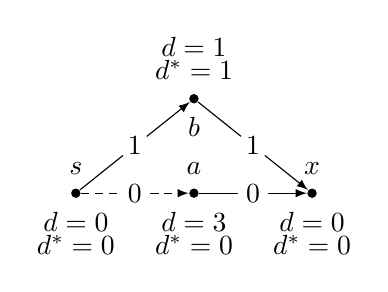
\begin{tikzpicture}
      \tikzset{>=latex} % arrow heads
      \node[fill=black,circle,inner sep=1.2pt] (s) at (0,0) {};
      \node[fill=black,circle,inner sep=1.2pt] (a) at (1.5,0) {};
      \node[fill=black,circle,inner sep=1.2pt] (b) at (1.5,1.2) {};
      \node[fill=black,circle,inner sep=1.2pt] (x) at (3.0,0) {};
      \draw[->,densely dashed] (s) -- (a) node[midway,fill=white,circle,inner sep=1pt] {0};
      \draw[->] (a) -- (x) node[midway,fill=white,circle,inner sep=1pt] {0};
      \draw[->] (s) -- (b) node[midway,fill=white,circle,inner sep=1pt] {1};
      \draw[->] (b) -- (x) node[midway,fill=white,circle,inner sep=1pt] {1};

      \node[above=0.05cm of s] {$s$};
      \node[above=0.05cm of a] {$a$};
      \node[below=0.05cm of b] {$b$};
      \node[above=0.05cm of x] {$x$};

      \node[below=0.05cm of s] {$d=0$};
      \node[below=0.05cm of a] {$d=3$};
      \node[above=0.35cm of b] {$d=1$};
      \node[below=0.05cm of x] {$d=0$};

      \node[below=0.35cm of s] {$d^*=0$};
      \node[below=0.35cm of a] {$d^*=0$};
      \node[above=0.05cm of b] {$d^*=1$};
      \node[below=0.35cm of x] {$d^*=0$};
   \end{tikzpicture}
   \caption{Problem case for pathfinding with distance functions.
      Here, $d$ satisfied a and c, with edge $e_{sa}$ tensioned,
      and $d' = 0$.
      While the approximation $d$ is \emph{sound} at $x$
      ($d(x)$ is correct),
      reconstructing a shortest path requires \emph{completeness}.}
   \label{fig:ibid:relaxation-completeness-issue}
\end{marginfigure}

\begin{theorem}
If either $w \geq 0$ and $d^*(x) < d'$,
or if $w > 0$ and $d^*(x) \leq d'$,
then $d(x) = d^*(x)$.
\label{thm:ibid-relaxation-complete}
\end{theorem}

\begin{proof}[Proof of Theorem~\ref{thm:ibid-relaxation-complete}]
Consider a true shortest path $p^*$ of length $d^*(x)$ from $s$ to $x$.
Due to our conditions,
all vertices $u$ before $x$ on $p^*$ have $d^*(u) < d'$.
By (\ref{eqn:ibid-relaxation-props}),
we have $d(s) = d^*(s) = 0$.
Consider each edge $e_{uv}$ in turn along $p^*$,
for which $d^*(u) + w(e_{uv}) = d^*(v)$.
For each, suppose that $d(u) = d^*(u)$.
Then we have $d(u) < d'$,
so that edge $e_{uv}$ must not be in tension.
Thus $d(v) \leq d(u) + w(e_{uv})$,
and by (\ref{eqn:ibid-relaxation-props}) we know $d(v) = d^*(v)$.
Therefore, we have $d(x) = d^*(s)$.
\end{proof}

\begin{theorem}
If either $w \geq 0$ and $d^*(x) < d'$,
or if $w > 0$ and $d^*(x) \leq d'$,
then a shortest path can be reconstructed backwards from $x$
by prepending the incoming edge $e_{uv}$ which minimizes
$d(u) + w(e_{uv})$ until $s$ is reached.
\label{thm:ibid-relaxation-reconstruct}
\end{theorem}

\begin{proof}[Proof of Theorem~\ref{thm:ibid-relaxation-reconstruct}]
We will show that for every such vertex $x$,
there exist a predecessor $u$ and incident edge $e_{uv}$
for which $d(u) + w(e_{uv}) = d(x)$.
It follows that $e_{uv}$ is on a shortest path to $x$.
This argument can then be applied recursively to $u$,
which must still satisfy the necessary conditions.
\end{proof}

\section{Bidirectional Search}
\label{sec:ibid:bidirectional}

One prominent technique for minimizing pathfinding computation for
single-pair problems
is bidirectional search.
In a bidirectional algorithm,
the distance $d_t$ to the target is calculated in a growing region
around the target vertex $t$
concurrently with the conventional source distance $d_s$ around $s$
(Figure~\ref{fig:ibid:example-bidirectional}).
Loosely speaking,
the search can terminate with a shortest path
once the two regions intersect.
The savings relative to a unidirectional search grow with the problem's
branching factor.
For roadmap graphs embedded in an ambient space,
this branching factor can be linear or exponential in the space's
dimension.
\begin{marginfigure}%
   \centering%
   \includegraphics[width=5cm]{figs/incbi-road-ne/singleshot/example-bidijkstra.png}%
   \caption{The bidirectional Dijkatra's algorithm
      computes $d_s$ around the source vertex
      and $d_t$ around the target vertex.
      Darker vertices have smaller $d$-values in their respective
      regions.
      The algorithm terminates after expanding a total of
      1,178,200 vertices using distance to balance expansions.}%
   \label{fig:ibid:example-bidirectional}%
\end{marginfigure}

The first bidirectional algorithm
was proposed by Dantzig \citep{dantzig1963linearprogramming},
and the first precisely described algorithm was presented by
Nicholson \citep{nicholson1966shortest}.
Implementation of a sound and efficient algorithm
turns on two important questions:
(a) when and how to terminate with a shortest path,
and (b) how to balance expansions from the two directions of the
search.

\subsection{Termination Conditions}
\label{sec:ibid:bidirectional-termination}

What is the equivalent to the completeness-based termination condition
described in Section~\ref{subsec:ibid-dijkstra-completeness}?

What happens upon an encounter between the forward and reverse searches?
Goldberg \citep{goldberg2005spexternalmemory}
discusses the correct termination condition for the 
Bidirectional Dijkstra algorithm.

A correct termination condition is surprisingly subtle,%
\marginnote{There were early incorrect attempts at a sound
termination condition
\citep{berge1965programminggamestransportation}.}
with several correct variations proposed
\citep{nicholson1966shortest, dreyfus1969appraisalsp,
pohl1969bidirectional, goldberg2005spexternalmemory}.
The difficulty stems from the fact that the first vertex to be
{\sc Closed} by the searches in both directions
need not lie on the shortest path
(Figure~\ref{fig:ibid:bidirectional-termination-issue}).

Key point, reason about edges!

See Algorithm~\ref{alg:ibid:bidirectional-termination}.

\begin{algorithm}[t]
   \caption{Bidirectional Termination Condition}
   \label{alg:ibid:bidirectional-termination}
   \begin{algorithmic}[1]
      \State On $u$ expanded in the foward search
         with $v$ already expanded in the backward search,
   \end{algorithmic}
\end{algorithm}

\begin{marginfigure}
   \centering
   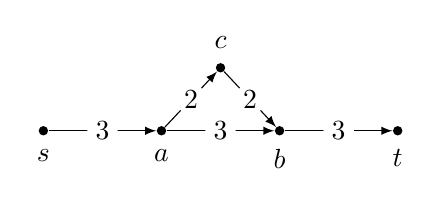
\begin{tikzpicture}
      \tikzset{>=latex} % arrow heads
      \node[fill=black,circle,inner sep=1.2pt] (s) at (0,0) {};
      \node[fill=black,circle,inner sep=1.2pt] (a) at (1.5,0) {};
      \node[fill=black,circle,inner sep=1.2pt] (b) at (3.0,0) {};
      \node[fill=black,circle,inner sep=1.2pt] (t) at (4.5,0) {};
      \node[fill=black,circle,inner sep=1.2pt] (c) at (2.25,0.8) {};
      \draw[->] (s) -- (a) node[midway,fill=white,circle,inner sep=1pt] {3};
      \draw[->] (a) -- (b) node[midway,fill=white,circle,inner sep=1pt] {3};
      \draw[->] (b) -- (t) node[midway,fill=white,circle,inner sep=1pt] {3};
      \draw[->] (a) -- (c) node[midway,fill=white,circle,inner sep=1pt] {2};
      \draw[->] (c) -- (b) node[midway,fill=white,circle,inner sep=1pt] {2};
      \node[below=0.05cm of s] {$s$};
      \node[below=0.05cm of a] {$a$};
      \node[below=0.05cm of b] {$b$};
      \node[below=0.05cm of t] {$t$};
      \node[above=0.05cm of c] {$c$};
   \end{tikzpicture}
   \caption{Simple illustration of a problem case for terminating
      a bidirectional search.
      With a balanced distance criterion,
      $c$ will be the first vertex expanded in both directions,
      but it does not lie on the shortest path.}
   \label{fig:ibid:bidirectional-termination-issue}
\end{marginfigure}

\subsection{Balancing Directions}
The general bidirectional algorithm leaves open the strategy
used to balance the progression of the two search directions.
Options based on alternating \citep{dantzig1963linearprogramming},
or selecting the direction with the smaller {\sc Open} distance
\citep{nicholson1966shortest}
or {\sc Open} (and finite) set cardinality
\citep{pohl1969bidirectional}
have been proposed.
Note that while some literature asserts that
these can be interleaved arbitrarily,
termination of the algorithm requires that each direction
be expanded at least once.
Our example problems use the balanced distance criterion.

\section{Incremental Search}
\label{sec:ibid:incremental}

How can we adapt the relaxation approach to the incremental setting?
And how can we recover the original algorithm from the more general one?

We can rely on just the consistency,
but not the upper bound part.
So now there are many solutions.
So we need to further constrain the graph to have
positive edge weights.

This stuff is more modern (1996, 2004).

A review is here: \citep{eppstein1999dynamic},
\citep{demetrescu2010dynamic}.

Talk about how this is centrally a restatement of the Dijktsra's ordering.
Bring in the invariant.

DynamicSWSF-FP \citep{ramalingam1996dynamicswsffp}.

How about this: \citep{frigioni2000dynamicsp}.

Revisit Bellman equation.

The central idea is that the search maintains the following invariant.
Note that this is a basic restatement of the distance function
ordering that underlies Dijkstra's algorithm.

Define $r$ and $d$,
what we mean by \emph{consistent},
and what $k$ is.

In general (no non-positive cycles),
the algorithm terminates.
The proof is that key values only increase (somehow).

All of the proofs in this section relate to
graphs with positive edge weights ($w > 0$),
with $k_{\ms{min}}$ the minimal key among inconsistent vertices.

\subsection{Approximation Soundness}

The theorems below are basically a soundness proof --
if our approximation yields values below a certain value,
they are known to be correct.
This is soundness of the approximation,
not of an algorithm per se.

\begin{theorem}
Any consistent vertex $x$ with $d[x] \leq k_{\ms{min}}$
has $d[x] = d^*(x)$.
\label{thm:ibid-dynamicswsffp-sound}
\end{theorem}

\begin{proof}[Proof of Theorem~\ref{thm:ibid-dynamicswsffp-sound}]
The proof relies upon a path construction described by
Lemma~\ref{lemma:ibid-dynamicswsffp-sound-conpath}.
We then show that $d[x]$ can be both
no less than $d^*(x)$
(Lemma~\ref{lemma:ibid-dynamicswsffp-sound-geq})
and no greater than $d^*(x)$
(Lemma~\ref{lemma:ibid-dynamicswsffp-sound-leq}).
\end{proof}

\begin{lemma}
For any consistent vertex $x$ with $d[x] \leq k_{\ms{min}}$,
there exists a path $p$ from $s$ to $x$
in which each vertex is consistent
and each edge $e_{uv}$ satisfies $d[u] + w(e_{uv}) = d[v]$.
\label{lemma:ibid-dynamicswsffp-sound-conpath}
\end{lemma}

\begin{proof}[Proof of Lemma~\ref{lemma:ibid-dynamicswsffp-sound-conpath}]
Construct the path $p$ as follows.
Initialize the path with the single vertex $x$.
Iteratively consider the first vertex $v$ on the path,
which is known to be consistent.
In the first case, if $v \neq s$,
then there exists a predecessor vertex $u$ and edge $e_{uv}$
with $d[u] + w(e_{uv}) = r(v)$.
Since $w > 0$ and $d[v] = r(v)$,
we have $d[u] < d[v] \leq d[x]$.
As a consequence,
$u$ is consistent;
prepend to the path the vertex $u$ and the edge $e_{uv}$,
and iterate.
In the second case, if $v = s$,
then we finish our construction of $p$.
Since the values $d[u]$ decrease monotonically
for all inserted vertices,
this process will terminate with a path $p$ beginning at $s$.
\end{proof}

\begin{lemma}
Any consistent vertex $x$ with $d[x] \leq k_{\ms{min}}$
has $d[x] \geq d^*(x)$.
\label{lemma:ibid-dynamicswsffp-sound-geq}
\end{lemma}

\begin{proof}[Proof of Lemma~\ref{lemma:ibid-dynamicswsffp-sound-geq}]
This follows directly from
Lemma~\ref{lemma:ibid-dynamicswsffp-sound-conpath}.
Since all vertices on the path are known consistent,
we must have $d[s] = 0$.
Further,
since the $d$-values across each edge in $p$
satisfy $d[u] + w(e_{uv}) = d[v]$,
it follows that $d[x] = \sum_{e \in p} w(e)$.
Therefore,
a path exists from $s$ to $x$ of length $d[x]$,
and so the true distance $d^*(x)$ must be upper-bounded by $d[x]$.
\end{proof}

\begin{lemma}
Any consistent vertex $v$ with $d[x] \leq k_{\ms{min}}$
has $d[x] \leq d^*(x)$.
\label{lemma:ibid-dynamicswsffp-sound-leq}
\end{lemma}

\begin{proof}[Proof of Lemma~\ref{lemma:ibid-dynamicswsffp-sound-leq}]
We demonstrate that $d[x] \leq d^*(x)$ by contradiction.
Suppose a vertex $x$ exists for which $d^*(x) < d[x]$.
Then there must exist a path $p'$ from $s$ to $x$ of length $d^*(x)$,
with $d^*(s) = 0$ and $d^*(u) + w(e_{uv}) = d^*(v)$ for each edge
in $p'$;
as a consequence,
we must have $d^*(v) < d[x]$ for all vertices $v$ on $p'$.
By Lemma~\ref{lemma:ibid-dynamicswsffp-sound-conpath},
we know that $s$ is consistent,
so $d[s] = 0$.
We will show that walking along
each edge $e_{uv}$ on $p'$ starting at $s$,
if $d[u] \leq d^*(u)$,
then $d[v] \leq d^*(v)$.

By definition,
we have $d[u] + w(e_{uv}) \geq r[v]$,
so that $d[u] - d^*(u) \geq r[v] - d^*(v)$.
Therefore,
it follows that $r[v] \leq d^*(v)$.
Since $k[v] \leq d^*(v)$,
it follows that $v$ is consistent,
so $d[v] \leq d^*(v)$.
We can replicate this logic down the path.
As a result,
it follows that $d[x] \leq d^*(x)$.
But this contraducts our supposition that $d^*(x) < d[x]$,
and therefore such a vertex $x$ cannot exist.
\end{proof}

\begin{marginfigure}%
   \centering%
   \subfloat[Initial search]{%
      \centering%
      \includegraphics[width=5cm]{figs/incbi-road-ne/singleshot/example-incuni-0.png}%
   }
   
   \subfloat[Replan search]{%
      \centering%
      \includegraphics[width=5cm]{figs/incbi-road-ne/singleshot/example-incuni-1.png}%
   }%
   \caption{Initial search: 1,287,897 expansions.
      Replan: 391,122 expansions.}%
   %\label{fig:ibid:example-bidirectional}%
\end{marginfigure}

\subsection{Approximation Completeness}

For bidirectional search,
it's also necessary to be able to prove that you have found
all vertices within a certain distance of the start.
Basically, this is a completeness proof --
if a distance exists below a certain value,
we will have found it.
This is completeness of the approximation,
not of an algorithm per se.

\begin{theorem}
Any vertex $x$ with $d^*(x) < k_{\ms{min}}$
has $d[x] = d^*(x)$.
\label{thm:ibid-dynamicswsffp-complete}
\end{theorem}

\begin{proof}[Proof of Theorem~\ref{thm:ibid-dynamicswsffp-complete}]
We show that $d[x]$ can be both
no less than $d^*(x)$
(Lemma~\ref{lemma:ibid-dynamicswsffp-complete-geq})
and no greater than $d^*(x)$
(Lemma~\ref{lemma:ibid-dynamicswsffp-complete-leq}).
\end{proof}

\begin{lemma}
Any vertex $x$ with $d^*(x) < k_{\ms{min}}$
has $d[x] \geq d^*(x)$.
\label{lemma:ibid-dynamicswsffp-complete-geq}
\end{lemma}

\begin{proof}[Proof of Lemma~\ref{lemma:ibid-dynamicswsffp-complete-geq}]
We show this by contradiction.
Suppose there exists a vertex $x$ with $d^*(x) < k_{\ms{min}}$
for which $d[x] < d^*(x)$.
Then $d[x] < k_{\ms{min}}$,
so $x$ must be consistent.
By Lemma~\ref{lemma:ibid-dynamicswsffp-sound-geq},
we must have $d[x] \geq d^*(x)$.
This contradicts our supposition.
\end{proof}

\begin{lemma}
Any vertex $x$ with $d^*(x) < k_{\ms{min}}$
has $d[x] \leq d^*(x)$.
\label{lemma:ibid-dynamicswsffp-complete-leq}
\end{lemma}

\begin{proof}[Proof of Lemma~\ref{lemma:ibid-dynamicswsffp-complete-leq}]
This proof proceeds in a similar way to that for
Lemma~\ref{lemma:ibid-dynamicswsffp-sound-leq}.
Construct a true shortest path from $s$ to $x$,
with $d^*$-values increasing monotonically from
$d^*(s) = 0$ to $d^*(x)$.
Consider each edge $e_{uv}$ in turn as follows.
Assume that $u$ is consistent,
with $d[u] \leq d^*(u)$.
Note that this is true for the first edge with $u = s$,
since with $0 \leq d^*(x)$,
we have $0 < k_{\ms{min}}$,
so that $s$ must is consistent with $r[s] = d[s] = d^*(s) = 0$.
Since $e_{uv}$ lies on a true shortest path,
we must have $d^*(u) + w(e_{uv}) = d^*(v)$,
and for all edges $d[u] + w(e_{uv}) \geq r[v]$.
Together, this implies that
$d^*(u) - d[u] \leq d^*(v) - r[v]$.
Our assumption that $d[u] \leq d^*(u)$
therefore implies that $r[v] \leq d^*(v)$.
Since $d^*(v) \leq d^*(x)$ and $d^*(x) < k_{\ms{min}}$,
we know that $v$ is consistent,
so we conclude that $d[v] \leq d^*(v)$,
and we can proceed to the next edge on the path.
We end with $v = x$,
so that $d[x] \leq d^*(x)$.
\end{proof}

\subsection{Incremental Bidirectional Search: The Algorithm}

Important: $s$ and $t$ must be distict!

\begin{theorem}
Define $E_{\ms{conn}}$ as the set of all edges $e_{uv}$ such that
$u$ is $s$-consistent with $d[s] \leq k_s$
and $v$ is $t$-consistent with $d[t] \leq k_t$.
If $k_s > 0$, $k_t > 0$,
and
$\min_{e \in E_{\ms{conn}}} \left( d_s[u] + w(e_{uv}) + d_t[v] \right)
   \leq k_s + k_t$,
then the path through $e_{uv}$ is a shortest path.
\label{thm:ibid-sound}
\end{theorem}

\begin{proof}[Proof of Theorem~\ref{thm:ibid-sound}]
We will prove this by contradiction.
Suppose that a path $p'$ exists with
$\mbox{len}(p') < \min_{e \in E_{\ms{conn}}} \left( d_s[u] + w(e_{uv}) + d_t[v] \right)$.
Then it must also be that
$\mbox{len}(p') < k_s + k_t$.
We will consider two cases.

First, consider the case where $k_s > \mbox{len}(p')$,
so that $k_s > d_s^*(t)$.
In this case,
the last edge $e_{ut}'$ on $p'$
has $d_s^*(u') < d_s^*(t) < k_s$;
by Theorem~\ref{thm:ibid-dynamicswsffp-complete},
$u'$ is therefore $s$-consistent with $d_s[u'] = d_s^*(u')$.
In addition,
since $k_t > 0$,
$t$ must be $t$-consistent with $d_t[t] = 0$.
Therefore,
it follows that $d_s^*(u') + w(e_{ut}') < d_s[u'] + w(e_{ut}')$,
which contradicts the supposition.

In the second case with $k_s \leq \mbox{len}(p')$,
identify on $p'$ the edge $e'_{uv}$ adjoining the vertices $u'$, $v'$
such that $d_s^*(u') < k_s \leq d_s^*(v')$.
(Since $k_s > 0$, this edge will exist.)
Since $d_s^*(u') < k_s$,
by Theorem~\ref{thm:ibid-dynamicswsffp-complete},
$u'$ is therefore $s$-consistent with $d_s[u'] = d_s^*(u')$.
Consider our supposition that
$d_s^*(u') + w(e_{uv}') + d_t^*(v') < k_s + k_t$.
Since $d_s^*(u') + w(e_{uv}') = d_s^*(v')$
and $k_s \leq d_s^*(v')$,
it follows that
$d_t^*(v') < k_t$.
Therefore,
by Theorem~\ref{thm:ibid-dynamicswsffp-complete},
$v'$ is $t$-consistent with $d_t[v'] = d_t^*(v')$.
As a consequence,
the edge $e'_{uv}$ must be in $E_{\ms{conn}}$.
Therefore,
$d_s^*(u') + w(e_{uv}') + d_t^*(v')
   < d_s[u'] + w(e_{uv}') + d_t[v']$,
which is a contradiction.
\end{proof}

\begin{marginfigure}%
   \centering%
   \subfloat[Initial search]{%
      \centering%
      \includegraphics[width=5cm]{figs/incbi-road-ne/singleshot/example-incbi-0.png}%
   }
   
   \subfloat[Replan search]{%
      \centering%
      \includegraphics[width=5cm]{figs/incbi-road-ne/singleshot/example-incbi-1.png}%
   }%
   \caption{Initial search: 1,181,616 expansions.
      Replan: 262,422 expansions.}%
   %\label{fig:ibid:example-bidirectional}%
\end{marginfigure}






\subsection{IBiD}

The main outline of IBiD is given in Algorithm~\ref{alg:ibid}.
IBiD conducts two independent DynamicSWSF-FP searches
(Algorithm~\ref{alg:ibid-two-dynamicswsffps}).

\begin{algorithm}[t]
   \caption{IBiD Outline}
   \label{alg:ibid}
   \begin{algorithmic}[1]
      \Procedure {Main} {\,}
         \State $\mbox{\sc InitializeSource}(); \; \mbox{\sc InitializeTarget}()$
         \State $Q_c \gets \emptyset$
            \Comment $\mbox{ key for } (u,v): d_s(u) + w(u,v) + d_t(v)$
         \Loop
            \While {not $\mbox{\sc TerminationCondition}()$}
               \If {$Q_s.\mbox{TopKey} < Q_t.\mbox{TopKey}$}
                     \Comment prioritize arbitrarily
                  \State $\mbox{\sc ProcessSourceQueue}(u)$
               \Else
                  \State $\mbox{\sc ProcessTargetQueue}(u)$
               \EndIf
               \State Ensure $(u,v) \in Q_c$ iff
                  $u \neq Q_s$, $v \neq Q_t$, key $\neq \infty$
            \EndWhile
            \State $(u_c,v_c) \gets Q_c.\mbox{Top}$
            \State $\pi \gets
               ( \mbox{walk } d_s \mbox{ from } u_c \mbox{ to } s )
               \cup
               ( \mbox{walk } d_t \mbox{ from } v_c \mbox{ to } t )$
            \State wait for edges $(u,v) \in E_{\ms{delta}}$ with changed weights $w(u,v)$
            \State $\mbox{\sc NotifyWeightChanges}(E_{\ms{delta}})$
         \EndLoop
      \EndProcedure
      \Function {TerminationCondition} {\,}
         \State $(u_c,v_c) \gets Q_c.\mbox{TopKey}$
            \Comment return False if $Q_c$ empty
         \If {$Q_s.\mbox{TopKey} + Q_t.\mbox{TopKey} < d_s(u_c) + w(u_c,v_c) + d_t(v_c)$}
            \State \Return False
         \EndIf
         \If {$Q_s.\mbox{TopKey} < d_s(u_c)$
               \mbox{\bf or} $Q_t.\mbox{TopKey} < d_t(v_c)$}
            \State \Return False
         \EndIf
         \State \Return True
      \EndFunction
      \Procedure {NotifyWeightChanges} {$E_{\ms{delta}}$}
         \ForAll {$(u,v) \in E_{\ms{delta}}$}
            \State $\mbox{\sc UpdateSourceDistance}(v)$
            \State $\mbox{\sc UpdateTargetDistance}(u)$
         \EndFor
         \State Ensure $(u,v) \in Q_c$ iff
            $u \neq Q_s$, $v \neq Q_t$, key $\neq \infty$
      \EndProcedure
   \end{algorithmic}
\end{algorithm}

{\floatevery{algorithm}{\setlength\hsize{16.85cm}}
\begin{algorithm}[t]
   \caption{As a bidirectional algorithm,
      IBiD conducts two independent DynamicSWSF-FP searches,
      one computing distance from the source vertex,
      and the other computing distance to the target vertex.}
   \label{alg:ibid-two-dynamicswsffps}
   \begin{minipage}[t]{8.2cm}
      \begin{algorithmic}[1]
         \Procedure {InitializeSource} {\,\!}
            \ForAll {$v \in V$}
               \State $d_s(v) \gets \infty; \;\; r_s(v) \gets \infty$
            \EndFor
            \State $r_s(s) \gets 0$
            \State $Q_s \gets \{ s \}$
               \Comment $\mbox{ key for } v: \min\big(r_s(v),d_s(v)\big)$
            \State $\mbox{\sc ProcessSourceQueue}()$
         \EndProcedure
         \Procedure {UpdateSourceDistance} {$v$}
            \If {$v \neq s$}
               \State $r_s(v) \gets \displaystyle\min_{u \in \mbox{\scriptsize Pred}(v)}
                  \big( d_s(u) + w(u,v) \big)$
            \EndIf
            \State Ensure $v \in Q_s$ iff $d_s(v) \neq r_s(v)$
         \EndProcedure
         \Procedure {ProcessSourceQueue} {\,\!}
            \State $u \gets Q_s.\mbox{Pop}()$
            \If {$r_s(u) < d_s(u)$}
                  \Comment over-consistent
               \State $d_s(u) \gets r_s(u)$
               \ForAll {$v \in \mbox{Succ}(u)$}
                  \State $\mbox{\sc UpdateSourceDistance}(v)$
               \EndFor
            \Else
                  \Comment under-consistent
               \State $d_s(u) \gets \infty$
               \ForAll {$v \in \mbox{Succ}(u) \cup u$}
                  \State $\mbox{\sc UpdateSourceDistance}(v)$
               \EndFor
            \EndIf
         \EndProcedure
         \algstore{ibid-two-dynamicswsffps}
      \end{algorithmic}
   \end{minipage}
   \quad
   \begin{minipage}[t]{8.2cm}
      \begin{algorithmic}[1]
         \algrestore{ibid-two-dynamicswsffps}
         \Procedure {InitializeTarget} {\,\!}
            \ForAll {$v \in V$}
               \State $d_t(v) \gets \infty; \;\; r_t(v) \gets \infty$
            \EndFor
            \State $r_t(t) \gets 0$
            \State $Q_t \gets \{ t \}$
               \Comment $\mbox{ key for } v: \min\big(r_t(v),d_t(v)\big)$
            \State $\mbox{\sc ProcessTargetQueue}()$
         \EndProcedure
         \Procedure {UpdateTargetDistance} {$u$}
            \If {$u \neq t$}
               \State $r_t(u) \gets \displaystyle\min_{v \in \mbox{\scriptsize Succ}(u)}
                  \big( w(u,v) + d_t(v) \big)$
            \EndIf
            \State Ensure $u \in Q_t$ iff $d_t(u) \neq r_t(u)$
         \EndProcedure
         \Procedure {ProcessTargetQueue} {\,\!}
            \State $v \gets Q_t.\mbox{Pop}()$
            \If {$r_t(v) < d_t(v)$}
                  \Comment over-consistent
               \State $d_t(v) \gets r_t(v)$
               \ForAll {$u \in \mbox{Pred}(v)$}
                  \State $\mbox{\sc UpdateTargetDistance}(u)$
               \EndFor
            \Else
                  \Comment under-consistent
               \State $d_t(v) \gets \infty$
               \ForAll {$u \in \mbox{Pred}(v) \cup v$}
                  \State $\mbox{\sc UpdateTargetDistance}(u)$
               \EndFor
            \EndIf
         \EndProcedure
      \end{algorithmic}
   \end{minipage}
\end{algorithm}
} % floatevery width adjustment

\section{Heuristic Search}
\label{sec:ibid:heuristic}

Heuristic methods such as the Graph Traverser
\citep{doran1966graphtraverser} were originally
applied to pathfinding problems in order to find non-optimal
solutions more economically.
These unidirectional methods proceed similarly to Dijkstra's algorithm,
but instead of prioritizing {\sc Open} vertices
based on their source distance $d_s$,
they use a target-directed heuristic function $h_t$.
Hart, Nilsson, and Raphael \citep{hart1968astar} discovered that
these approaches can be combined ($d_s + h_t$) to yield
an admissible algorithm (A*) for the shortest-path problem,
as long as $h_t$ meets certain conditions.

\paragraph{Example problem.}
\begin{marginfigure}%
   \centering%
   \includegraphics[width=5cm]{figs/incbi-road-ne/singleshot/example-astar.png}%
   \caption{A* search.
      532,880 expansions.}%
   \label{fig:ibid:example-astar}%
\end{marginfigure}
See Figure~\ref{fig:ibid:example-astar}.
For the purpose of calculating vertex heuristics,
geographic coordinates were projected onto a 2D plane using the
scale at the midpoint latitude ($41.25^\circ$)
resulting in a projecting error of less than 0.3\%.
The maximum transit speed is 30.11 m/s.

Attempts to provide a bidirectional algorithm which incorporates
heuristics generally take one of three approaches.
\cdnote{I need to deep-dive here to write this correctly.}

First,
front-to-front methods
could evaluate the heuristic between all pairs in the two
{\sc Open} sets.
Expensive.

Second,
perform two heuristic-informed searches,
and account for the connection problem via a complex
termination condition.
Not necessarily efficient.
(Pohl cites Berge?)
Missile analogy.

Third,
waste (same heuristic function).

Concept of waste \citep{pohl1969bidirectional}.
I think this subsumes A*.

Talk about the 94 paper \citep{ikeda1994betterroutes}
expressing A* as a search on
the waste graph.

As a potential function.
Also Goldberg \citep{goldberg2005spexternalmemory}.

To integrate: \citep{dechter1984bfsastaropt}.

\paragraph{Example problem.}
\begin{marginfigure}%
   \centering%
   \includegraphics[width=5cm]{figs/incbi-road-ne/singleshot/example-heurbidijkstra.png}%
   \caption{Bidirectional A* search.
      515,588 expansions.}%
   \label{fig:ibid:example-heurbidijkstra}%
\end{marginfigure}
See Figure~\ref{fig:ibid:example-heurbidijkstra}.

\subsection{The Zero-Weight Problem}

Talk about how a perfect potential leads to zero waste,
which breaks incremental search.
This motivates the lexocraphically sorted key approach.

\subsection{Incremental Heuristic Search}

Apply waste to incremental search to get
incremental heuristic search.

Lifelong Planning A* \citep{koenig2004lpastar}.

\section{Other Stuff}

\subsection{Examples}

See Figure~\ref{fig:incbi-lpastar-fig1-heurchange}
and Figure~\ref{fig:incbi-lpastar-fig1}.

\begin{figure}
   \centering%
   
   \includegraphics{build/incbi-lpastar-fig1/lpastar-heurnone-original}%
   \;\;%
   \includegraphics{build/incbi-lpastar-fig1/incbi-heurnone-original}%
   
   \vspace{0.2cm}
   
   \includegraphics{build/incbi-lpastar-fig1/lpastar-heurhalf-original}%
   \;\;%
   \includegraphics{build/incbi-lpastar-fig1/incbi-heurhalf-original}%
   
   \vspace{0.2cm}
   
   \includegraphics{build/incbi-lpastar-fig1/lpastar-heurfull-original}%
   \;\;%
   \includegraphics{build/incbi-lpastar-fig1/incbi-heurfull-original}%
   
   \caption{Illustration of behavior of IBiD on a single
      (non-incremental) shortest path problem.
      At left, IBiD uses the unidirectional start-side expansion
      strategy.
      At right, IBiD uses the bidirectional distance-balanaced
      expansion strategy.
      Start and goal heuristic functions are available;
      the unidirectional search uses a potential function based
      on the goal heuristic,
      and the bidirectional search a potential function using
      the average heuristic.
      IBiD is run with three different potential function weights:
      0.0 (top), 0.5 (middle), and 1.0 (bottom).
      IBiD therefore preforms equivalently to
      Dijkstra's algorithm (top-left),
      Bidirectional Dijkstra's (top-right),
      A* (bottom-left),
      and Bidirectional A* (bottom-right).}
   \label{fig:incbi-lpastar-fig1-heurchange}
\end{figure}

\begin{figure}
   \centering%
   
   \includegraphics{build/incbi-lpastar-fig1/lpastar-heurfull-original}%
   \;\;%
   \includegraphics{build/incbi-lpastar-fig1/lpastar-heurfull-changed}%
   
   \vspace{0.2cm}
   
   \includegraphics{build/incbi-lpastar-fig1/incbi-heurfull-original}%
   \;\;%
   \includegraphics{build/incbi-lpastar-fig1/incbi-heurfull-changed}%
   
   \caption{IBiD with only source-side expansions and a goal-side
      heuristic (top) proceeds identically to Lifelong Planning A*,
      performing 37 expansions on the original world (left)
      followed by 18 expansions over 14 vertices on the chanced
      world (right).
      IBiD with distance-balanced expansions and an average
      potential (bottom)
      performs 30 expansions on the original world
      followed by 18 expansions over 15 vertices on the changed
      world.}
   \label{fig:incbi-lpastar-fig1}
\end{figure}

\begin{figure*}
   \centering%
   
   \begin{tabular}{ccc}
      \specialcell{\includegraphics[width=5cm]{figs/incbi-road-ne/singleshot/pgoalnone-balfwd.png}\\556,209 expansions}
      &
      \specialcell{\includegraphics[width=5cm]{figs/incbi-road-ne/singleshot/pavgnone-baldist.png}\\319,938 expansions}
      &
      \specialcell{\includegraphics[width=5cm]{figs/incbi-road-ne/singleshot/pavgnone-balcard.png}\\281,413 expansions}
      \vspace{0.3cm}
      \\
      \specialcell{\includegraphics[width=5cm]{figs/incbi-road-ne/singleshot/pgoalhalf-balfwd.png}\\297,414 expansions}
      &
      \specialcell{\includegraphics[width=5cm]{figs/incbi-road-ne/singleshot/pavghalf-baldist.png}\\206,625 expansions}
      &
      \specialcell{\includegraphics[width=5cm]{figs/incbi-road-ne/singleshot/pavghalf-balcard.png}\\178,929 expansions}
      \vspace{0.3cm}
      \\
      \specialcell{\includegraphics[width=5cm]{figs/incbi-road-ne/singleshot/pgoalfull-balfwd.png}\\82,915 expansions}
      &
      \specialcell{\includegraphics[width=5cm]{figs/incbi-road-ne/singleshot/pavgfull-baldist.png}\\95,759 expansions}
      &
      \specialcell{\includegraphics[width=5cm]{figs/incbi-road-ne/singleshot/pavgfull-balcard.png}\\69,218 expansions}
      \vspace{0.5cm}
   \end{tabular}
   
   \caption{Comparison between various heuristic strengths and
      balancing strageties on a single-pair road network problem.
      A path with shortest transit time is sought.
      The heuristic strength varies from no heuristic (top)
      to a full-strength heuristic (bottom).
      At left, a foward-only balancer is used, so that the
      top-left is equivalent to Dijkstra's algorithm,
      and the bottom-left is equivalent to A*.
      The middle column uses a balanced distance strategy.
      The right column uses a balanced cardinality strategy.}
   \label{fig:incbi-road-ne}
\end{figure*}

\subsection{LazySP Selector Experiments}

\begin{figure}
   \centering
   \includegraphics{build/incbi-sq/all-even}
   \caption{Across a selection of articulated robot planning instances,
      using the Even edge selector.
      Algorithms are
      \protect\tikz{\protect\node[fill=black!30,draw=black,postaction={pattern=north west lines}]{};}\;LPA*,
      \protect\tikz{\protect\node[fill=black!20,draw=black]{};}\;IBiD,
      and \protect\tikz{\protect\node[fill=black!30,draw=black,postaction={pattern=north east lines}]{};}\;Reverse LPA*.
      Results shown are cumulative search time.
      }
\end{figure}

\begin{figure}
   \centering
   \includegraphics{build/incbi-road-ne/stats}
   \caption{Road network incremental results.
      Algorithms are
      \protect\tikz{\protect\node[fill=black!30,draw=black,postaction={pattern=north west lines}]{};}\;LPA*,
      \protect\tikz{\protect\node[fill=black!20,draw=black]{};}\;IBiD,
      and \protect\tikz{\protect\node[fill=black!30,draw=black,postaction={pattern=north east lines}]{};}\;Reverse LPA*.
      }
\end{figure}

\begin{figure}
   \centering
   \includegraphics{build/incbi-sq/herbbin0}
   
   \includegraphics{build/incbi-sq/herbbin0-lambda}
   \caption{Problem: \texttt{herbbin0}.
      Lines are:
      \protect\tikz{\protect\draw[thick] (0,0) -- (0.15,0.15);} no heuristic,
      \protect\tikz{\protect\draw[densely dashed] (0,0) -- (0.15,0.15);} start heuristic,
      \protect\tikz{\protect\draw[densely dashdotted] (0,0) -- (0.15,0.15);} avg heuristic,
      \protect\tikz{\protect\draw[densely dotted] (0,0) -- (0.15,0.15);} goal heuristic.
      }
\end{figure}

\begin{figure*}
   \centering
   \includegraphics{build/incbi-sq/herbbookshelf0}
   \includegraphics{build/incbi-sq/herbbookshelf1nom}
   
   \includegraphics{build/incbi-sq/herbbookshelf0-lambda}
   \includegraphics{build/incbi-sq/herbbookshelf1nom-lambda}
   \caption{Problems: \texttt{herbbookshelf0} (left), texttt{herbbookshelf1nom} (right).}
\end{figure*}

\begin{figure*}
   \centering
   \includegraphics{build/incbi-sq/workcellef}
   \includegraphics{build/incbi-sq/workcellij}
   
   \includegraphics{build/incbi-sq/workcellef-lambda}
   \includegraphics{build/incbi-sq/workcellij-lambda}
   \caption{Problems: \texttt{workcellef} (left), \texttt{workcellij} (right).}
\end{figure*}

\subsection{Implementation Details}

Other implementations:
\citep{alberts1998softwaredynamicgraph}.

\chapter{Maximizing Utility in Motion Planning}
\label{chap:utility}

Up to this point,
we have considered general optimization problems on graphs:
given an edge weight function $w : E \rightarrow \mathbb{R}$
which is expensive to evaluate,
how can arrive at a minimizing solution path as quickly as possible?
We saw in Chapters~\ref{chap:lazysp} that the LazySP algorithm
can take advantage of different edge selectors in order to minimize
the number of such evaluations,
and Chapter~\ref{chap:ibid} discussed the IBiD incremental search
algorithm for efficiently solving the intervening dynamic
pathfinding problem.

In this chapter,
we will ask a more fundamental question
-- what objective should we be optimizing in the first place?
Chapter~\ref{chap:roadmaps} laid out the functionals
$x_{\ms{valid}}$ and $x_{\ms{int}}$
capturing the feasible and optimal motion planning problems,
respectively.
But as we report in the introduction,
robots must allocate limited resources between planning
motions and subsequently executing them.
Existing approaches for motion planning in such high-dimensional
spaces,
including sampling-based, asymptotically optimal and anytime planners,
risk either quickly returning a solution that is expensive to execute,
or spending too much planning effort improving an existing solution.

The primary contribution of this chapter is to imbue 
lazily-evaluated sampling-based approaches
with a \emph{utility function}
which incorporates both planning and execution cost in its objective.
Reasoning over utility provides the planner
with a means to trade off between these costs using a single input
parameter,
as well as a natural termination condition.
Furthermore,
treating planning cost explicitly
provides a natural way to accommodate task-specific planning
heuristics.
The planner performs well on a set of benchmark tasks,
and is particularly amenable to caching
%\scnote{Is caching a standard thing in the roadmap planning context?
%Or if not, do you intend to explain it further?}
and parallelization.

\section{Motivation and Related Work}

\begin{figure}
   \centering
   \begin{tikzpicture}
      \node[inner sep=0cm] at (1.9,6.25) {\includegraphics{build/pvx-graph}};
      \node[inner sep=0cm] at (2.08,2.65) {\includegraphics[width=3.51cm]{build/multiple-sets}};
      \node[inner sep=0cm] at (6.5,4.77)
         {\includegraphics[width=4.25cm]{figs/herbarm-snapshot-cropped.png}};
         
      \node[fill=white,inner sep=2pt,anchor=west] at (7.5,7.5) {\scriptsize planning: 2.9s};
      \node[fill=white,inner sep=2pt,anchor=west] at (7.5,7.2) {\scriptsize execution: 5.7s};
      \draw[thick,->] (7.5,7.35) -- (7.0,6.5);
      
      \node[fill=white,inner sep=2pt,anchor=west] at (7.0,2.0) {\scriptsize planning: 2.4s};
      \node[fill=white,inner sep=2pt,anchor=west] at (7.0,1.7) {\scriptsize execution: 12.4s};
      \draw[thick,->] (7.8,2.2) -- (8.05,3.2);
   \end{tikzpicture}
   \caption[A robot reaching to grab a book
      must allocate limited resources between planning and executing its motion.
      Our planner reasons over a user-defined utility function (top~left)
      to explicitly trade-off between these two significant sources
      of cost.
      As its roadmap search discovers valid edges,
      it mediates between
      high-cost edges that are fast to find
      and low-cost edges that require significant planning
      directly via their prospective utilities.
      Because the planner accepts arbitrary estimators
      for planning cost,
      it can naturally exploit both caching and geometric structure in
      $\mathcal{C}$.
   ]{
      A robot reaching to grab a book
      must allocate limited resources between planning and executing its motion.
      Our planner reasons over a user-defined utility function (top~left)
      to explicitly trade-off between these two significant sources
      of cost.
      As its roadmap search (right) discovers valid edges
      (\protect\tikz{\protect\draw[thick] (0,0) -- (0.15,0.15);}),
      it mediates between
      high-cost edges that are fast to find~%
      (\protect\tikz{\protect\draw[blue,ultra thick] (0,0) -- (0.15,0.15);})
      and low-cost edges that require significant planning~%
      (\protect\tikz{\protect\draw[green,ultra thick] (0,0) -- (0.15,0.15);})
      directly via their prospective utilities.
      Because the planner accepts arbitrary estimators
      for planning cost,
      it can naturally exploit both caching and geometric structure in
      $\mathcal{C}$ (bottom left).}
   \label{fig:fig1}
\end{figure}

\scnote{General Comment: I did not quite follow how 'marginal' utility applies here. I'm sure it is not the term from probability.
Do you use marginal to indicate that you optimize for utility?}

Autonomous robots in the real world
must carefully allocate limited resources (e.g. time or energy)
between planning motions and executing them.
A robot that favors execution
risks prematurely committing to an uneconomical path, whereas
one that favors planning risks unduly delaying execution 
due to incessant small refinements.
This tradeoff is especially relevant for working with
or around humans, who are simultaneously 
unaccommodating of long pauses
and of wild and unpredictable motion.

Most planning algorithms pick a side and stick to it.

Randomized algorithms such as the
PRM~\citep{kavrakietal1996prm}
and RRT~\citep{lavallekuffner1999rrt},
strive to find feasible paths while minimizing planning cost,
falling in the $A_1$ category of the planning vs. execution
plot (Figure~\ref{fig:fig1}, we will formalize notation 
in Section \ref{sec:utility}).
Techniques such as caching, parallelization \citep{ichnowski2012prrt},
and lazy evaluation \citep{bohlin2000lazyprm}
are often used to further reduce online planning cost.
%They use post-processing like path 
%shortcutting to reduce execution effort albeit exclusively 
%focusing on minimizing planning effort.

Optimal algorithms
such as FMT*~\citep{janson2015fmtstar}
exclusively optimize for execution
cost ($A_2$ in Figure~\ref{fig:fig1}), 
and often use techniques such as informed heuristics to improve
planning efficiency as a secondary objective.
Graph search approaches \citep{hart1968astar}
can guarantee solution optimality
with respect to a chosen discretization,
and often incorporate a parameter ($A_3$) such as inflation
\citep{pohl1970weightedastar}
or an execution cost bound \citep{stern2014}
that reduces the algorithm's runtime at the expense of optimality.
However,
it can be difficult to set these parameters for a particular domain.

Anytime algorithms $A_4$
for continuous
\citep{karaman2011samplingoptimal, gammell2015bitstar, hauser2015lazy}
or discrete
\citep{likhachev2004arastar} problems
come the closest, providing a sequence of solutions
with decreasing execution cost.
However, they are best suited for \emph{uncertain}
planning budgets, and as a consequence of this uncertainty
incur planning cost producing
solutions that never get used.
It can also be difficult to decide when to terminate them.
We wish to do better.

\paragraph{Expressing the Planning vs. Execution Tradeoff.}
Our goal is to devise an algorithm that \emph{explicitly} reasons over both planning
and execution cost. Our algorithm should behave like an optimal algorithm 
if execution cost is critical, and like a randomized algorithm if planning
cost is critical. Crucially, it should behave like a mix between the two 
if both are important to the user.

To enable this, we borrow a concept from the AI community~\citep{ruml2007bugsy},
allowing the user to specify a \emph{utility function} describing
their planning vs. execution tradeoff
(illustrated via isocontours in Figure~\ref{fig:fig1}).
We describe some examples and theoretical properties of this
function in Section \ref{sec:utility}, but it can be arbitrarily nuanced, 
or extremely simple,
e.g. a linear function that sums planning and execution cost.
We argue that utility is an essential metric
by which to evaluate motion planners.

Considering this utility function, we make the following observations: 
(1) we can update estimates of utility online during planning;
(2) we can estimate execution cost of a path
(e.g. path length or energy) quite accurately.
%\scnote{The idea I get reading is that it is the utility 
%function that lets you estimate execution cost quite accurately, which I guess
%is not the idea.}.

However, our key insight is that we can
\emph{estimate the planning cost} in domains
where this cost is dominated by the effort of
verifying the validity of edges via collision-checking.
This is true for most real-world robot motion planning problems
where 80-95\% of the planning time
is dominated by collision-checking.

\paragraph{Lazily Evaluated Marginal Utility Roadmas.}
When combined, these insights enable a planning approach which
reason explicitly over utility using online estimates.
This leads naturally to the
Lazily Evaluated Marginal Utility Roadmaps (LEMUR) planner
(Section~\ref{sec:roadmaps}).
LEMUR takes as input a parameterized utility function $U_\lambda$ 
and attempts to find and validate a solution path
that maximizes that utility.

LEMUR has several advantages over anytime planners.
First,
the user's utility function provides a natural termination condition
-- the planner returns a solution when no alternatives provide
a prospective improvement in utility.
Second, the planner does not waste effort generating
intermediate solutions.

The performance of LEMUR is also easier to tune to a particular
problem domain.
In particular,
the parameter it uses to mediate between costs is
the user's utility function itself.
It is therefore unnecessary to tune inflation factors or
trajectory optimization budgets to achieve good performance.

We compare LEMUR to several sampling-based and anytime planners
across a set of motion planning problems
in Section~\ref{sec:experiments}.

LEMUR's ability to accept an arbitrary planning effort model
enables it to be customized to different domains.
In Chapter \ref{chap:family},
we discuss such a model specific to problems over a family of
C-space subsets.
A prime example of this is multi-step manipulation tasks
in which the C-space changes with each object grasp and placement.
This allows computation to be efficiently cached and reused.

The combination of
marginal utility, lazy evaluation, and roadmap methods
work in concert and are adaptable to new domains.
Section~\ref{sec:utility:discussion} concludes the chapter with a discussion
of potential extensions and applications of our algorithm.

\section{Utility in Motion Planning}
\label{sec:utility}

We consider the optimal motion planning problem
as described in Chapter~\ref{chap:roadmaps}.
We consider a cost function
$x: \Xi \rightarrow \mathbb{R}^+$
which measures path quality --
in our case, the cost of executing a solution path.
Examples of $x$ include the path's length
or the time or energy required to execute it.
$x$ is commonly treated as part of the problem specification;
each instance admits a path(s) with optimal execution cost $x^*$.

A sound motion planner $A$ accepts a problem instance
and yields a valid solution path $\xi$
with execution cost $x[\xi]$.
We are also interested in measuring the planning cost incurred by
the algorithm itself
via a real-valued performance metric $p$.
Examples of $p$ include the number of iterations or
collision checks performed,
or the amount of time or energy consumed by the planner.
Figure~\ref{fig:utility-contours} provides an illustration of
these two costs on the plane.

In general,
a planner endeavoring to reduce the execution cost of its solution path
must incur additional planning cost to do so.
While a wealth of planning approaches are available in the literature,
few attempt to capture this underlying tradeoff directly.
We propose to do so via a \emph{utility function}.
Utility functions were first exploited by the
Best-first Utility-Guided Search (BUGSY) algorithm
\citep{ruml2007bugsy,burns2013bugsy}
to order vertex expansions during a
conventional graph search.
We propose to apply a similar insight to motion planners
which use lazy evaluation.

\subsection{Utility Functions}
\label{subsec:utility-functions}

A utility function $U$ is a scalar-valued function
over both $p$ and $x$
which provides the motion planner with
the \emph{utility} of returning a
solution path with execution cost $x$ calculated after
incurring planning cost $p$
(Figure~\ref{fig:utility-contours}).
Utility functions are applicable to a wide range of planning regimes
and often emerge readily from the problem domain.
A utility function also naturally reconciles cost functions
$p$ and $x$ that are in different units
(e.g. collision checks and path length).
We follow the convention that utility is to be maximized
(whereas cost is to be minimized).

\begin{figure}
   \centering
   \subfloat[A utility function over $p,x$]{%
      \centering
      \includegraphics{build/pvx-utility}
      \label{fig:utility-contours:pvx-utility}
   }%
   \quad%
   \subfloat[Maximizing utility with parameterized or anytime planners]{%
      \centering
      \includegraphics{build/pvx-utility-anytime}
      \label{fig:utility-contours:pvx-utility-anytime}
   }%
   
   \subfloat[First feasible]{%
      \centering
      \includegraphics{build/pvx-sm-firstfeas}
      \caption{}
      \label{fig:utility-contours:pvx-sm-firstfeas}
   }%
   \quad%
   \subfloat[Bounded cost]{%
      \centering
      \includegraphics{build/pvx-sm-xbudget}
      \label{fig:utility-contours:pvx-sm-xbudget}
   }%
   \quad%
   \subfloat[Planning budget]{%
      \centering
      \includegraphics{build/pvx-sm-pbudget}
      \label{fig:utility-contours:pvx-sm-pbudget}
   }%
   \caption{Contours of a utility function $U(p,x)$.
      Also some examples of simple utility functions
      relevant to related work.}
   \label{fig:utility-contours}
\end{figure}

While $U$ may be any function,
there are certain properties that we can expect from any reasonable
choice.
In particular,
\begin{equation}
   \nabla U \leq \mathbf{0}.
\end{equation}
This follows from the following arguments
(Figure~\refsub{fig:utility-contours}{pvx-utility}).
If $\partial_x U$ were positive,
it would be beneficial for a planner to return a path with larger
execution cost.
Similarly,
if $\partial_p U$ were positive,
it would be beneficial for a planner to artificially delay returning
a given solution path.

\cdnote{Say something about local structure, dot product, etc etc.}

Several common planning regimes can be expressed exactly as
utility functions.
For example,
requesting a planner to return a solution as quickly as possible
irrespective of its execution cost corresponds to the first-feasible
utility in Figure~\refsub{fig:utility-contours}{pvx-sm-firstfeas}.
Bounded-cost planners such as Potential Search (PTS) \citep{stern2014}
address problems in which a solution below a prescribed cost $x_b$ is
desired as quickly as possible (Figure~\refsub{fig:utility-contours}{pvx-sm-xbudget}).
The converse formulation requests the lowest-cost path
within a fixed planning budget $p_b$
(Figure~\refsub{fig:utility-contours}{pvx-sm-pbudget}).

It is instructive to consider how existing types of planners
might be applied if utility is to be maximized.
Many planners
($A_3$ in Figure~\refsub{fig:utility-contours}{pvx-utility-anytime})
take parameters which profoundly affect both the
quality of their solutions and the planning cost they incur.
The range parameter of the RRT \citep{lavallekuffner1999rrt}
and the inflation factor in Weighted A* \citep{pohl1970weightedastar}
are common examples of this.
However,
it is difficult to choose the values for these parameters;
they must often be learned empirically in a way that is
specific both to the planner and to the problem instance.

Anytime planners such as
Anytime Repairing A* \citep{likhachev2004arastar}
and RRT* \citep{karaman2010rrtstar}
return a low-quality solution quickly,
and then continually return improved solutions as more planning
is performed ($A_4$ in Figure~\refsub{fig:utility-contours}{pvx-utility-anytime}).
Applying an anytime planner to a utility-maximization problem suffers
from two drawbacks.
First,
an outside process must enforce an appropriate termination condition.
While this may be straightforward for simple utilities
(e.g. from Figures~\refsub{fig:utility-contours}{pvx-sm-firstfeas}-%
\refsub{fig:utility-contours}{pvx-sm-pbudget}),
a nontrivial utility function requires a complex termination model
which must be learned in a problem-specific way.
Second,
scarce planning resources are typically allocated on low-quality
intermediate paths which will go unused.

\begin{algorithm}[t]
\caption{Lazily Evaluated Utility-Guided Search Outline}
\label{alg:utility-search-outline}
\begin{algorithmic}[1]
\For {iteration $i \in 1, 2, \dots$}
   \State $\bar{p}_i \leftarrow$
      planning cost incurred so far
   \State $\Xi_i \leftarrow$ set of paths to consider at iteration $i$
   \State $\grave{p}_i : \Xi_i \rightarrow \mathbb{R}^+$
      \Comment additional planning cost estimator
   \State $\hat{x}_i : \Xi_i \rightarrow \mathbb{R}^+$
      \Comment execution cost estimator
   \State $\xi_i = \argmax_{\xi \in \Xi_i}
      U\!\left( \; \bar{p}_i \! + \! \grave{p}_i(\xi), \; \hat{x}_i(\xi) \; \right)$
      \label{line:outline-argmax}
   \State \Return $\xi_i$
      if $\grave{p}_i( \xi_i ) = 0$
   \State evaluate $\xi_i$
      \Comment incurs requisite planning cost
\EndFor
\end{algorithmic}
\end{algorithm}

\subsection{Outline of Lazily Evaluated Utility-Guided Search}

We endeavor to marry utility functions with lazy motion planning.
Lazy path evaluation is well-suited to domains with expensive
validity checking,
and is a common technique \citep{bohlin2000lazyprm, cohen2014narms}.
Here,
we provide the general outline of a class of algorithms which
takes as input a utility function $U$
and selects paths to evaluate based on estimates of their utility.

The planner maintains estimates $\hat{p}$ and $\hat{x}$
of the planning and execution costs, respectively,
for each of a set of prospective trajectories $\Xi$.
While a prospective path's execution cost may be easy for a planner
to estimate via commonly used heuristics,
incorporating estimates of the planning cost
to be incurred by the algorithm itself is more difficult.
While the planner is running,
we can decompose its planning estimate $\hat{p}$ for a prospective
path $\xi$ into two components:
\begin{equation}
   \hat{p}(\xi) = \bar{p} + \grave{p}[\xi]
\end{equation}
that is,
the measured planning cost elapsed $\bar{p}$
and the estimated remaining planning cost $\grave{p}$.

\begin{figure}
   \centering
   \subfloat[Planning cost estimates]{%
      \centering
      \includegraphics{build/p-estimates}
      \label{fig:pvx-linear-discounting:p-estimates}
   }%
   \quad%
   \subfloat[Evolution of path utilities]{%
      \centering
      \includegraphics{build/pvx-linear-discounting}
      \label{fig:pvx-linear-discounting:pvx-linear-discounting}
   }
   \caption{A planner reasoning with a linear utility function
      chooses to first evaluate trajectory $\xi_1$.
      After incurring planning cost $\bar{p}$
      (less than it had expected),
      it finds that it is more expensive than expected;
      some of the planning work has also adjusted the estimates
      for nearby trajectory $\xi_2$.
      However,
      the estimated remaining planning costs $\grave{p}$
      for all other unaffected trajectories have remained constant.
      Therefore, the relative utilities have also not changed.
      As such, a planner need not re-order any trajectories whose
      estimated planning cost to go has not changed.}
   \label{fig:pvx-linear-discounting}
\end{figure}

Consider the planner outline in
Algorithm~\ref{alg:utility-search-outline}.
At each iteration $i$,
the planner has incurred $\bar{p}_i$ planning cost so far.
It considers a set of prospective paths $\Xi_i$
(left unspecified).
It also has available estimators for each path's execution cost
$\hat{x}_i$
and its remaining planning cost
$\grave{p}_i$.
Note that these estimators can change between iterations --
for example,
a path's remaining planning estimate becomes 0 once it is
fully evaluated,
and its execution effort becomes $\infty$ if it is found to be
infeasible.
Estimates for other paths which share segments may also be
updated (Figure~\ref{fig:pvx-linear-discounting}).
\scnote{Similar concern. At this stage I (as a new reader) am still having difficulty figuring out what 
exactly the planning effort implies, and understanding that they are related, might help that }

Using these estimators,
the planner selects among $\Xi_i$
the path $\xi_i$ which maximizes the given utility function $U$.
If no planning cost remains, it is returned;
otherwise,
it is evaluated,
incurring the requisite planning cost.
Note that this algorithm terminates naturally,
and therefore avoids incurring planning cost seeking out
low-quality intermediate solutions.

The outline in Algorithm~\ref{alg:utility-search-outline} is able to
broadly capture the behavior of a number of well-known planning
algorithms.
For example, consider the symmetric bidirectional variant of the
common RRT-Connect algorithm \citep{kuffner2000rrtconnect}.
At each iteration $i$,
the algorithm samples a configuration $q_i$ uniformly from
$\mathcal{C}$.
The candidate path that it then selects for evaluation
(Figure~\ref{fig:rrt})
is identical to the path which minimizes
the first-feasible utility function
(Figure~\refsub{fig:utility-contours}{pvx-sm-firstfeas})
among $\Xi_i$,
the set of all prospective paths constrained to pass through $q_i$.
It is therefore unsurprising that RRT-Connect typically completes
with remarkably little planning cost
(albeit often with poor execution cost).

%\ssnote{From Sidd (early on):
%reference visibility prm: explicitly reason about what I'm
%implicitly reasoning about.}

\begin{figure}
   \centering
   \subfloat[RRT snapshot.]{%
      \centering
      \includegraphics{build/rrt}
      \label{subfig:rrt}
   }%
   \quad%
   \subfloat[Utility]{%
      \centering
      \includegraphics{build/pvx-rrt}
      \label{subfig:pvx-rrt}
   }
   \caption[
      At each iteration $i$,
      the simplified bidirectional
      RRT-Connect planner
      always selects among all paths constrained to pass through
      the sampled configuration $q_i$
      that which minimizes the necessary planning cost only.
   ]{At each iteration $i$,
      the simplified bidirectional
      RRT-Connect \citep{kuffner2000rrtconnect} planner
      always selects among all paths constrained to pass through
      the sampled configuration $q_i$
      that which minimizes the necessary planning cost only.}
   \label{fig:rrt}
\end{figure}

\subsection{Linear Combinations and Elapsed Planning Cost}

One particularly common class of utility functions consists of the
a linear combinations of $p$ and $x$:
\begin{equation}
   U_l(p,x) = -w_p \, p - w_x \, x
\end{equation}
for non-negative $w_p$, $w_x$.
Despite their simplicity,
such utilities are able to capture regimes
which span the gamut between minimizing planning and execution costs.
In particular,
if $w_p$ and $w_x$ are chosen to bring their metrics into the same
total task units with equal weight,
$U_l$ commands the planner to directly minimize the sum of the two.
This is particularly appropriate in regimes where the robot is to
immediately execute the planned path,
and total task cost is to be minimized.

In addition to their applicability,
a utility function that is a linear combination
also exhibits a desirable cost-discounting property which a planner
can exploit.

\begin{theorem}
   \label{thm:linear-elapsed}
   If the utility function can be written as $U(p,x) = - w_p \, p - f(x)$,
   then the path $\xi_i$ selected by
   Algorithm~\ref{alg:utility-search-outline}
   (line~\ref{line:outline-argmax})
   is independent of the elapsed planning cost $\bar{p}$.
\end{theorem}

\begin{proof}[Proof of Theorem~\ref{thm:linear-elapsed}]
   We have:
   \begin{align}
      \xi_i &= \argmax_{\xi \in \Xi_i}
      \Big[ \, U\big( \, \bar{p}_i \! + \! \grave{p}_i[\xi], \; \hat{x}_i[\xi] \big) \Big] \\
      &= \argmax_{\xi \in \Xi_i}
      \Big[ \,  U\big( \, \grave{p}_i[\xi], \; \hat{x}_i[\xi] \big) - w_p \, \bar{p}_i \, \Big] \\
      &= \argmax_{\xi \in \Xi_i}
      \Big[ \, U\big( \, \grave{p}_i[\xi], \; \hat{x}_i[\xi] \big) \Big]
   \end{align}
\end{proof}

In other words, the utilities of all prospective paths $\Xi_i$
are discounted the same amount
(Figure~\refsub{fig:pvx-linear-discounting}{pvx-linear-discounting}).

Because the planner maximizes $U_l$ at each iteration,
it is therefore completely characterized by a single parameter:
\begin{equation}
   w_p = \lambda_U \quad w_x = 1 - \lambda_U \quad
   \lambda_U \in [0,1]
\end{equation}
This parameter uniquely describes the relative tradeoff between
minimizing planning and execution cost.
It is often inherent in the problem setting,
or easily elicited from users.

\subsection{Linear Combinations and the Parameter Selection Problem}

\cdnote{Resolve duplication between this and
(a) Section~\ref{subsec:utility-functions}
and (b) the accompanying figure caption.}
Consider applying a parameterized planner $A(\eta)$
to the problem of maximizing a convex combination utility $U_l$.
Such a planner may take an explicit parameter,
such as the inflation factor $\epsilon$ in Weighted A*,
or it may be a termination condition for an anytime planner
such as an optimization time budget.
The performance of $A$ for different values of $\eta$ \scnote{People may have a hard time looking back to be sure 
$\eta$ represents the planner parameters. Maybe make that moren explicit?}
produces a locus on the $p,x$ plane
(Figure~\refsub{fig:convex}{pvx-convex}).
The utility achieved by any particular planner realization $A(\eta)$
corresponds to a line (Figure~\refsub{fig:convex}{amvu-convex}):
\begin{equation}
   - U_A(\lambda_U,\eta)
   = \lambda_U \, p_A(\eta)
   + (1\!-\!\lambda_U) \, x_A(\eta).
\end{equation}
Invoking such a planner for utility maximization
requires that the parameter $\eta$ be set appropriately
as a function of $\lambda_U$.
An ideal $\eta$ schedule would follow the convex hull of all
lines in Figure~\refsub{fig:convex}{amvu-convex}:
\begin{equation}
   \eta^*_A(\lambda_U) = \argmax_{\eta} U_A(\lambda_U,\eta).
   \label{eqn:oracle-param-schedule}
\end{equation}
The locus of utility-maximizing planner parameters
corresponds to the lower-left convex hull of $A$
(bolded in Figure~\refsub{fig:convex}{pvx-convex}).

Determining a suitable such schedule
$\eta_A(\lambda_U)$,
that is, the \emph{parameter selection problem},
is difficult to solve for many planners across a wide range of
problem domains.
Tuning (e.g. setting a shortcutting time budget)
is often required to achieve good utility in practice.
One advantage of the utility-aware planner outlined in
Algorithm~\ref{alg:utility-search-outline}
is that it operates directly on the problem's utility function itself.

\begin{figure}
   \centering
   \subfloat[p-vs-x plot.]{%
      \centering
      \includegraphics{build/pvx-convex}
      \label{fig:convex:pvx-convex}
   }%
   \quad%
   \subfloat[Corresponding utility plotot.]{%
      \centering
      \includegraphics{build/lamvu-convex}
      \label{fig:convex:amvu-convex}
   }
   \caption{A parameterized planner A maximizes a linear combination
      utility (for some value $\lambda_U$)
      along the subset of parameter values which
      constitute the lower-left convex hull of the $p$-vs-$x$ plot (left).
      Each realization of planner A for a particular parameter value
      (a point at left) corresponds to a line at right,
      which shows the utility achieved for that realization
      over various values of $\lambda_U$
      (negative utility shown, lower is better).
      Applying a parameterized planner for utility maximization
      requires selecting $\eta$ according to $\lambda_U$
      in such a way that the realized utility approximates
      the lower bound across all parameter choices (right).}
   \label{fig:convex}
\end{figure}

\section{Marginal Utility on Roadmaps}
\label{sec:roadmaps}

The Lazily Evaluated Marginal Utility Roadmaps (LEMUR) motion planner
is an implementation of utility-guided search which unifies
lazy evaluation, marginal utility, and roadmap methods.
It follows the general outline from
Algorithm~\ref{alg:utility-search-outline}
and exploits several properties and assumptions that are
common in motion planning for articulated robots.
The planner considers paths constrained to a roadmap graph $G$
defined a priori in $\mathcal{C}$,
and resembles repeated invocations of the LazySP algorithm
from Chapter~\ref{chap:lazysp}
on progressively densified roadmaps.
The set of continuous paths $\Xi$ considered by the planner is
therefore restricted to the set of paths $\Pi$ on the roadmap.

%\cdnote{Add taxonomy/atlas plot of planner comparing to
%existing planners (e.g. from proposal doc).}

\subsection{Cost Estimates Additive over Edges}

Performing lazy evaluations entails repeated searches over
roadmap paths.
To make this efficient,
we commit to path cost estimators
$\grave{p}_i(\pi)$ and $\hat{x}_i(\pi)$
that are additive over edges:
\begin{equation}
   \grave{p}_i(\pi) = \sum_{e \in \pi} \grave{p}_i(e)
   \quad\mbox{and}\quad
   \hat{x}_i(\pi) = \sum_{e \in \pi} \hat{x}_i(e).
\end{equation}

Many common performance metrics meet this criteria,
including path length, execution time under velocity limits,
and number of collision checks.
These two edge estimators are provided as input to the planner
in the form of an edge cost model $\mathcal{M}$.
Utility maximization at each iteration $i$ is then
equivalent to solving
a shortest-path problem over the roadmap with the following
edge weight function:
\begin{equation}
   w_i(e) = w_p \, \grave{p}_i(e) + w_x \, \hat{x}_i(e).
   \label{eqn:edge-weight}
\end{equation}

\subsection{Locality of Estimator Updates}

The LEMUR algorithm evaluates a single roadmap edge $e_i$
at each iteration $i$.
Most common cost estimate models exhibit \emph{update locality}:
evaluating an edge does not affect the estimates of other edges
on the roadmap.
This allows for two optimizations.
First,
due to Theorem~\ref{thm:linear-elapsed},
the per-iteration edge weight function $w_i$
can be stored as a single scalar value $w$ per edge,
with only a single edge weight updated per iteration.
Second,
an incremental shortest-path algorithm,
as described in detail in Chapter~\ref{chap:ibid},
can be used to efficiently search for candidate paths.

Certain cost estimate models exhibit an approximate form of
update locality.
For example, the estimates for an edge $e_{ab} = (v_a, v_b)$
often incorporate the validity of the configurations
at its end vertices $v_a$ and $v_b$,
which are shared with other adjacent roadmap edges.
For example, if evaluating $e_{ab}$ finds that $v_a$ is invalid,
then the estimates $\hat{x}$ and $\grave{p}$ for all edges
adjacent to $v_a$ may also be updated.
However,
the number of edge weights to be updated remains small
compared to the size of the roadmap.

\begin{algorithm}[t]
\caption{Lazily Evaluated Marginal Utility Roadmaps}
\label{alg:lemur}
\begin{algorithmic}[1]
\Procedure {LEMUR}{$q_{\ms{start}}, q_{\ms{goal}}, x,
   \mathcal{M}.\grave{p}, \mathcal{M}.\hat{x}, \lambda_p$}
\State $G \leftarrow$ graph with
   $V = \{ q_{\ms{start}}, q_{\ms{goal}} \}$
   and $E = \emptyset$
\State $w : E \rightarrow \mathbb{R}^{+}$
   \Comment mutable edge weight function
\For {iteration $i \in 1, 2, \dots$}
   \State $\pi_i = \displaystyle\argmin_{\pi \in \Pi(G)} 
      \mbox{len}\left(\pi, w\right)$
      \Comment incremental search
   \If {$\pi_i$ is {\bf null}}
      \State $V_{\ms{new}}, E_{\ms{new}} \leftarrow$ new densified roadmap batch
      \State $G.V \stackrel{\tiny +}\leftarrow V_{\ms{new}};
         \;\; G.E \stackrel{\tiny +}\leftarrow E_{\ms{new}}$
      \State $w(e) \leftarrow \lambda_p \, \grave{p}_i(e) + (1\!-\!\lambda_p) \, \hat{x}_i(e)
         \; \forall \; e \in E_{\ms{new}}$
      \State {\bf continue}
   \EndIf
   \If {$\pi_i$ is fully evaluated}
      \State \Return $\pi_i$
   \EndIf
   \State $e_i \leftarrow$ select unevaluated edge from $\pi_i$
   \State evaluate $e_i$
   \State $\hat{x}(e_i) \leftarrow x(e_i); \;\; \grave{p}(e_i) \leftarrow 0$
      \Comment e.g. evaluate fully
   \State $w(e_i) \leftarrow
      \lambda_p \, \grave{p}(e_i) + (1\!-\!\lambda_p) \, \hat{x}(e_i)$
\EndFor
\EndProcedure
\end{algorithmic}
\end{algorithm}

\subsection{The Algorithm}

The LEMUR planner is shown in Algorithm~\ref{alg:lemur}.
The planning query consists of the configurations
$q_{\ms{start}}, q_{\ms{goal}}$
along with the evaluation function $x$ which determines the true
execution cost of an edge (e.g. $\infty$ if invalid).
As $x$ is usually expensive to compute,
the planner is provided with an ensemble edge cost model $\mathcal{M}$
with two independent estimators:
$\hat{x}(e)$ estimating the value of $x(e)$,
and $\grave{p}(e)$ estimating the planning cost required to
compute $x(e)$ itself.
The planner is also given the user's utility tradeoff
$\lambda_p \in [0,1]$ as a planner parameter.

The algorithm begins with an initial roadmap graph $G$
comprised of the query vertices
and an edge weight function $w$ over the (initially empty) set
of edges.
At each iteration $i$,
the roadmap is searched for a path $\pi_i$
which maximizes estimated utility according to $\lambda_p$.
This search uses an incremental search algorithm
(our experiments use the IBiD algorithm from Chapter~\ref{chap:ibid}).
If no such path exists
(i.e. all paths have infinite weight),
the roadmap is expanded with a new batch of vertices and edges.
The algorithm is agnostic to the roadmap construction method used;
our experiments use Halton sequences with an $r$-disk connection rule.

If the path $\pi_i$ has been fully evaluated,
then (a) it requires no additional planning cost,
and (b) no prospective path on $G$ has a larger estimated utility
than $\pi_i$.
Therefore, the algorithm immediately terminates and returns $\pi_i$.

Otherwise,
an edge $e_i$ on $\pi_i$ that has not been fully evaluated
is selected for evaluation.
Our experiments simply select the unevaluated edge
nearest to an end of the path,
although other selection strategies are possible.
Once evaluated,
the estimates for $e_i$ are recomputed,
modifying its edge weight according to (\ref{eqn:edge-weight})
for future iterations.
For example, if it is fully evaluated,
its remaining planning cost becomes zero.

\begin{algorithm}[t]
\caption{Simple Edge Cost Model $\mathcal{M}_{\ms{simple}}$}
\label{alg:model-simple}
\begin{algorithmic}[1]
\Function{$\grave{p}_{\ms{\textup{simple}}}$}{$e$}
   \Comment remaining plan-cost estimator
   \If {$e$ is unevaluated}
      \State \Return $\sum_{q \in e} \grave{p}_{\ms{config}}(q)$
   \Else
      \State \Return $0$
   \EndIf
\EndFunction
\Function{$\hat{x}_{\ms{\textup{simple}}}$}{$e$}
   \Comment exec-cost estimator
   \If {$e$ is unevaluated or valid}
      \State \Return $||e||$
   \Else
      \State \Return $\infty$
   \EndIf
\EndFunction
\end{algorithmic}
\end{algorithm}

\subsection{Ensemble Edge Cost Models}
\label{subsec:lemur:ensemble-edge-cost-models}

The ensemble edge cost model $\mathcal{M}$
which provides the estimators $\grave{p}(e)$ and $\hat{x}(e)$
depends on the implementation of the evaluation function $x(e)$
and is therefore specific to the the planning domain.
Suppose that the true execution cost $x$ of each edge
is either its edge length if valid, or $\infty$ otherwise.
Further,
suppose that determining its validity requires performing
discrete collision checks interpolated along the edge at some
resolution.
The cost model $\mathcal{M}_{\ms{simple}}$ shown in
Algorithm~\ref{alg:model-simple}
captures this case.
Note that this model uses the free-space assumption:
unevaluated edges are assumed to be valid.

\subsection{Analysis}

LEMUR is an application of marginal utility to lazy roadmap methods,
and therefore it shares a similar structure
to Lazy PRM \citep{bohlin2000lazyprm}.
In fact, in the case that $\lambda_p=0$,
LEMUR reduces to Lazy PRM
(for appropriate choice of the edge selection and evaluation strategy),
since both algorithms will only consider execution cost when choosing
candidate paths.

LEMUR conducts its searches over any progression of
successively densified roadmaps over $\mathcal{C}$.
Recent work has demonstrated that roadmaps constructed via
randomized \citep{karaman2011samplingoptimal}
or deterministic \citep{janson2015deterministicsampling} sampling
techniques
(for appropriate choice of the roadmap parameters)
endow motion planners which conduct systematic searches thereon
with desirable properties such as resolution
and probabilistic completeness.
If the estimates $\grave{p}$ and $\hat{x}$
are both finite for unevaluated edges,
LEMUR is guaranteed to conduct such a systematic search.

The cost model's estimators $\grave{p}$ and $\hat{x}$ can each be any
function.
However,
it is often the case that bounds are available for both estimates
relative to the true execution cost of the edge $x$.
For example,
both may be proportional to the Euclidean length of the edge
(e.g. the estimated planning cost may be proportional to the number
of interpolated configurations to be checked).
Such bounds allow for a suboptimality bound on the execution cost
of the path returned by LEMUR
(Theorem~\ref{thm:suboptimality}).

\begin{theorem}[Execution Suboptimality of LEMUR]
   \label{thm:suboptimality}
   If the cost model $\mathcal{M}$
   satisfies
   \begin{equation}
      \hat{x}(e) \leq \alpha_x x(e)
      \mbox{ and }
      \grave{p}(e) \leq \alpha_p x(e)
      \label{eqn:suboptimality-conditions}
   \end{equation}
   for some constants $\alpha_x$ and $\alpha_p$,
   then the execution cost of the path returned by LEMUR
   with $\lambda_p < 1$
   is within a factor $\epsilon$ of the
   execution-optimal path on $G$,
   with $\epsilon = \frac{\lambda_p}{1 - \lambda_p}\alpha_p + \alpha_x$.
\end{theorem}

\begin{proof}[Proof of Theorem~\ref{thm:suboptimality}]
   Suppose that LEMUR returns path $\pi_L$.
   Since it is fully evaluated, it has weight
   $w(\pi_L) = (1\!-\!\lambda_p) x(\pi_L)$.
   Now, consider an execution-optimal path $\pi^*$ on $G$,
   which had
   $w(\pi^*) = \lambda_p \grave{p}(\pi^*) + (1\!-\!\lambda_p) \hat{x}(\pi^*)$
   at the point the algorithm terminated.
   Since $\pi_L$ was chosen over $\pi^*$,
   we have that $w(\pi_L) \leq w(\pi^*)$.
   Due to (\ref{eqn:suboptimality-conditions}),
   it follows that
   \begin{equation}
      (1\!-\!\lambda_p) x(\pi_L)
      \leq
      \lambda_p \alpha_p x(\pi^*) + (1\!-\!\lambda_p) \alpha_x x(\pi^*)
   \end{equation}
   Because we have $\lambda_p < 1$,
   we then have:
   \begin{equation}
      x(\pi_L)
      \leq
      \left( \frac{\lambda_p}{1-\lambda_p} \alpha_p + \alpha_x \right)
      x(\pi^*).
   \end{equation}
\end{proof}

\subsection{Suitability for Caching}

LEMUR searches a sequence of progressively densified roadmaps in
$\mathcal{C}$.
Analysis of the performance of lazy search for asymptotically-optimal
regimes \citep{hauser2015lazy}
has identified the nearest-neighbor queries required to construct
the roadmap itself as a significant component of planning cost.
We exploit two factors to mitigate this.
First,
because LEMUR endeavors to maximize utility (and therefore terminates),
its asymptotic behavior is of less importance.
Second,
we commit to roadmaps that are
(a) deterministic and
(b) independent of the
distribution of obstacles
(e.g. $r$-disk or $k$-nearest roadmaps).
This allows us the option to to amortize the cost of constructing
each batch of the roadmap across all planning queries performed by
the robot.
In our experiments,
we present timing results with and without the roadmap cache
(the same cache is used across all problem instances).

Beyond the roadmap structure itself,
edge validity state can be persisted across planning queries
yielding a multi-query planner
that is similar to the Lazy PRM or
Experience graphs \citep{phillips2012egraphs}.
We briefly discuss how to accommodate a changing configuration space in
Chapter~\ref{chap:family}.

\begin{figure}
   \centering
   \subfloat[RRT (Hybrid)]{%
      \includegraphics{build/lemur-sq/schedule-rrt}
      \label{subfig:schedule-rrt}
   }%
   \;\;%
   \subfloat[BIT*]{%
      \includegraphics{build/lemur-sq/schedule-bitstar}
      \label{subfig:schedule-bitstar}
   }%
   \;\;%
   \subfloat[LEMUR]{%
      \includegraphics{build/schedule-lemur}
      \label{subfig:schedule-lemur}
   }%
   \caption{Schedule of parameters for three of the algorithms
      compared.
      The hybrid RRT-Connect and BIT* are both anytime planners.
      The parameter learned was the algorithm termination time after
      the first returned path.
      The LEMUR algorithm does not require tuning;
      we used $\lambda_p = \lambda_U$ in our experiments.}
   \label{fig:herbarm-schedules}
\end{figure}

\begin{figure*}
   \begin{widepage}
   \begin{center}
   
   \includegraphics{build/filmstrip}

   \caption[Illustration of three trajectories generated by LEMUR
      on instance 6 from our experiments.
      The planner was initialized with the parameters
      $\lambda_p = 0, 0.5, \mbox{ and } 1$;
      the same roadmap was used.
      By increasing $\lambda_p$, the planner prefers minimizing
      planning cost at the expense of more costly solution paths.
   ][-30cm]{x}
   \label{fig:filmstrip}

   \end{center}
   \end{widepage}

   \vspace{0.1in}
   \smallskip\noindent\small Figure \ref{fig:filmstrip}:
      Illustration of three trajectories generated by LEMUR
      on instance 6 from our experiments.
      The planner was initialized with the parameters
      $\lambda_p = 0, 0.5, \mbox{ and } 1$;
      the same roadmap was used.
      By increasing $\lambda_p$, the planner prefers minimizing
      planning cost at the expense of more costly solution paths.
\end{figure*}

%\begin{figure*}
%   \centering   
%   \includegraphics{build/lemur-sq/chimp-master}
%   \caption[]{Experimental results across CHIMP motion planning
%      instances for a 7-DOF robot arm.}
%\end{figure*}

\section{Experiments}
\label{sec:experiments}

We conducted experiments for a robotic platform armed with a
7 DOF Barrett WAM manipulator \citep{salisbury1988wam}.
We used the FCL collision checker \citep{jiapan2012fcl} with a
resolution of 0.01 rad.
We considered three single-query instances in a tabletop
manipulation scenario
%(scene from Figure~\ref{fig:herbarmmultithread-master})
and three single-query instances from a bookshelf scenario
(Figure~\ref{fig:filmstrip}).
Planners were evaluated against a range of utility functions
trading off between path length (rad) and planning time (sec),
with $\lambda_U = 0.5$ corresponding to an equal weighting
when executing at 1.0 rad/sec.

\begin{figure}
   \centering
   \includegraphics{build/lemur-sq/herbbin0}
   \caption[
      Comparison of measured planning time $p$ and solution
      execution cost $x$ for the first step of the HERB table-clearing task.
      Results for four parameterized planners are shown:
      RRT-Connect, BIT*, Lazy~ARA*, and LEMUR.
      The LEMUR results show the effect of adjusting the $\lambda_p$
      tradeoff parameter from $0$ to $0.99$.
      The results for other planners show the effect of changing the
      total optimization time after the first returned solution.
      Also shown for reference are the contours for the
      $\lambda_U = 0.50$ utility function (i.e. 1~rad =~1~sec).
   ]{Comparison of measured planning time $p$ and solution
      execution cost $x$ for the first step of the HERB table-clearing task.
      Results for four parameterized planners are shown:
      RRT-Connect~(\protect\tikz{\protect\node[fill=red,draw=black]{};}),
      BIT*~(\protect\tikz{\protect\node[fill=green,draw=black]{};}),
      Lazy~ARA*~(\protect\tikz{\protect\node[fill=cyan,draw=black]{};}),
      and LEMUR~(\protect\tikz{\protect\node[fill=black!90,draw=black]{};}).
      The LEMUR results show the effect of adjusting the $\lambda_p$
      tradeoff parameter from $0$ (lower right) to $0.99$ (upper left).
      The results for other planners show the effect of changing the
      total optimization time after the first returned solution.
      Also shown for reference are the contours for the
      $\lambda_U = 0.50$ utility function (i.e. 1~rad =~1~sec).
      }
\end{figure}

We implemented LEMUR
as a planner for
the Open Motion Planning Library (OMPL) \citep{sucan2012ompl}.
We used the 7D Halton sequence to generate a low-dispersion
point set adjusted by an offset drawn uniformly
from $\mathcal{C}$.
Each roadmap batch consists of 10,000 vertices,
and the $r$-disk connection radius decreased from 2.0 rad
at the first batch in proportion to the Halton dispersion bound.
%When cached, the first 5 batches are stored on disk ($\approx$ 50MB).
Runtime memory usage was reduced by interpolating and allocating
within-edge states lazily during the search.
The planning parameter was chosen as $\lambda_p = \lambda_U$.

We compared LEMUR against
RRT-Connect \citep{kuffner2000rrtconnect}
%LBKPIECE \citep{sucan2008kpiece},
and Batch Informed Trees (BIT*) \citep{gammell2015bitstar}
as implemented in OMPL version 1.1.0
with default parameters.
To address maximal-utility problems,
RRT-Connect was augmented with the default OMPL
path shortcutter.
For each planner,
the optimization budget before termination
as a function of $\lambda_U$
was learned to maximize average utility across the instances
(Figure~\ref{fig:herbarm-schedules}).

\begin{figure}
   \centering
   \includegraphics{build/lemur-sq/workcellfg}
   \caption[Comparison of measured planning time $p$ and solution
      execution cost $x$ for the FG step of the workcell task.
      Results for four parameterized planners are shown:
      RRT-Connect, BIT*, Lazy~ARA*, and LEMUR.
      The LEMUR results show the effect of adjusting the $\lambda_p$
      tradeoff parameter from $0$ to $0.99$.
      The results for other planners show the effect of changing the
      total optimization time after the first returned solution.
      Also shown for reference are the contours for the
      $\lambda_U = 0.50$ utility function (i.e. 1~rad =~1~sec).
   ]{Comparison of measured planning time $p$ and solution
      execution cost $x$ for the FG step of the workcell task.
      Results for four parameterized planners are shown:
      RRT-Connect~(\protect\tikz{\protect\node[fill=red,draw=black]{};}),
      BIT*~(\protect\tikz{\protect\node[fill=green,draw=black]{};}),
      Lazy~ARA*~(\protect\tikz{\protect\node[fill=cyan,draw=black]{};}),
      and LEMUR~(\protect\tikz{\protect\node[fill=black!90,draw=black]{};}).
      The LEMUR results show the effect of adjusting the $\lambda_p$
      tradeoff parameter from $0$ (lower right) to $0.99$ (upper left).
      The results for other planners show the effect of changing the
      total optimization time after the first returned solution.
      Also shown for reference are the contours for the
      $\lambda_U = 0.50$ utility function (i.e. 1~rad =~1~sec).
      }
\end{figure}

We ran 50 trials for each planner,
with different random seeds.
The results are shown in Figure~\ref{fig:lemur:sq-herb-master}.
We collected results for versions of LEMUR with and without
nearest neighbor caching,
with time breakdowns for each shown in
Figure~\ref{fig:lemur:sq-herb-timing}.

\begin{figure}
   \centering
   \includegraphics{build/lemur-sq/chimp-valve-drc001-20131221-102450p936-CBRT}
   \caption[Comparison of measured planning time $p$ and solution
      execution cost $x$ for the first step of a CHIMP valve turning task.
      Results for four parameterized planners are shown:
      RRT-Connect, BIT*, Lazy~ARA*, and LEMUR.
      The LEMUR results show the effect of adjusting the $\lambda_p$
      tradeoff parameter from $0$ to $0.99$.
      The results for other planners show the effect of changing the
      total optimization time after the first returned solution.
      Also shown for reference are the contours for the
      $\lambda_U = 0.50$ utility function (i.e. 1~rad =~1~sec).
   ]{Comparison of measured planning time $p$ and solution
      execution cost $x$ for the first step of a CHIMP valve turning task.
      Results for four parameterized planners are shown:
      RRT-Connect~(\protect\tikz{\protect\node[fill=red,draw=black]{};}),
      BIT*~(\protect\tikz{\protect\node[fill=green,draw=black]{};}),
      Lazy~ARA*~(\protect\tikz{\protect\node[fill=cyan,draw=black]{};}),
      and LEMUR~(\protect\tikz{\protect\node[fill=black!90,draw=black]{};}).
      The LEMUR results show the effect of adjusting the $\lambda_p$
      tradeoff parameter from $0$ (lower right) to $0.99$ (upper left).
      The results for other planners show the effect of changing the
      total optimization time after the first returned solution.
      Also shown for reference are the contours for the
      $\lambda_U = 0.50$ utility function (i.e. 1~rad =~1~sec).
      }
\end{figure}

The relative performance between the planners varies
significantly between the six instances considered.
For example, BIT* performs very well on some instances
(e.g. nos. 2 and 6),
whereas it takes more than 100 seconds on average to discover
a path for instance 5.
The latter three (bookshelf) instances appear to pose particular
difficulty for the RRT;
the constrained space and cubbies may result in its trees
getting stuck easily.

As expected,
loading its roadmap from a cache
significantly speeds up LEMUR (by 4s - 15s on these instances).
As shown in Figure~\ref{fig:lemur:sq-herb-timing},
a large majority of the cached algorithm's runtime is spent
collision checking.
The path produced by LEMUR is independent of this caching,
so their utility curves meet at $\lambda_U = 0$
(when only solution quality is considered).
This condition also corresponds to the behavior of the Lazy PRM.

Across the six motion planning instances,
we found that LEMUR placed consistently among the best performers
across the range of utility functions.

\section{Discussion}
\label{sec:utility:discussion}

As robots take on more complex and deliberative tasks,
it is essential that they balance their computational and
physical efficiency.
Utility functions provide a natural way to represent this
inherent tradeoff between planning and execution
in motion planning.
The LEMUR planner relies directly on this utility
to guide its search for such a balance.

LEMUR relies on a domain-specific ensemble cost model to
estimate the planning and execution costs of prospective motions.
The parameter(s) of these models,
such as the expected cost of a collision check,
are easier to measure than corresponding parameters needed by
other planners.

%What happens if our planning estimate is not accurate?
%Reasons for this:
%(a) it doesn't account for search time, or other planning time
%(b) our estimate of collision checking cost is only an estimate.

While LEMUR is agnostic to the class of roadmap used,
methods which use deterministic sampling
\citep{lavalle2004deterministic, janson2015deterministicsampling}.
have distinct advantages with regard to caching of collision state
within and between planning episodes and parallel processors.
Furthermore,
by committing to a particular set of roadmap instantiations,
we can potentially optimize them offline \citep{salzman2014sparsification}
to exhibit good behavior on a particular robot.

%Discuss cute tangent angle line segment never-gonna-do-better
%thing!

\cdnote{
We could maximize expected utility
by simply choosing estimators which are themselves expectations.
}

\cdnote{
How to accommodate inaccurate estimates?
Planning estimates are always inaccurate.
How to incorporate constants e.g. search time?
Suppose it is inevitable that you're wrong about your planning estimate.
Here ares some ways that we could fix it.
Perhaps artificially inflate the per-batch search cost?
}

\chapter{Planning over Configuration Space Families}
\label{chap:family}

To this point,
we have considered motion planning problems in which a path is sought
within a fixed valid subset
$\mathcal{C}_{\ms{free}} \subset \mathcal{C}$
In Chapter~\ref{chap:lazysp},
we described a lazy search algorithm which is suited to domains in
which determining the weight of an edge
-- perhaps due to expensive set membership tests --
is expensive.
Chapter~\ref{chap:utility} discussed the concept of utility to
motion planning,
and showed examples of its application to single-query motion
planning problems.

However,
many applications exhibit structure beyond simple binary belief over
configuration validity.
In this chapter,
we introduce the \emph{family motion planning problem},
a generalization of the motion planning problem to a family of sets
over $\mathcal{C}$.
We then show how such a problem over familes can be represented
as in the utility function framework,
and given as input to the LEMUR motion planner described
in Chapter~\ref{chap:utility}.

This chapter proceeds as follows.
Section~\ref{sec:family:related-work} surveys related work.
In Section~\ref{sec:family:families-in-manipulation},
we motivate these the family motion planning problem
from the standpoint of manipulation tasks.
Section~\ref{sec:family:formulation} formulates the problem
generally.
We describe our approach in Section~\ref{sec:family:approach},
which details how the family problem can be represented
as a utility model that can be used by LEMUR.
The chapter concludes with experimental results on multi-step
manipulation tasks in Section~\ref{subsec:family:app-multi-step}.

\section{Related Work}
\label{sec:family:related-work}

The topic of reusing planning computation
between similar motion planning problems
has been extensively studied in the literature.
We include here a broad survey of existing approaches.
%the application sections
%(Section~\ref{subsec:family:app-multi-step}
%-- \ref{subsec:family:dynamic-environments}) also include
%relevant references to prior work.

\paragraph{Exact Algorithms.}
Exact planning methods construct explicit obstacles
directly in the configuration space.
Many such approaches allow for precomputation of primitives,
such as bitmaps \citep{kavraki1995cspacefft}
or C-space primitives for different workspace obstacles
\citep{newmanbranicky1991cspacetransforms}.
More recently,
Lien and Lu \citep{lien2009similarobstacles} describe a method to
build a PRM around obstacles in a database,
and then reposes them in a new world.
As described in Section~\ref{subsec:roadmaps:sensitive},
the exact approach is not easily applicable to articulated robots
with complex mappings from workspace to C-space.

\paragraph{Accommodating Dynamic Subsets in Sampling-Based Planning.}
Strong recent interest in sampling-based planning
has lead to the development of a number of approaches to handle
environments in which $\mathcal{C}_{\ms{free}}$ changes over time.
If a given discretization is asserted a priori,
this problem setting is similar to the dynamic shortest path problem
from Chapter~\ref{chap:ibid};
we refer the reader to that chapter for a review of related work.
Many sampling-based approaches attempt to prune and grow
the discretizations itself in response to these changes,
such as the Dynamic RRT \citep{ferguson2006drrt},
the Reconfigurable Random Forest (RRF)
\citep{li2002incrementalprmmanagement},
and the Lazy Reconfiguration Forest
\citep{gayle2007lazyreconfigforest}.
%We do the lazy thing as well (built into our planner).
%None of these reason about the structure of the configuration space.
However, these approaches do not reason explicitly about the
structure of the configuration space,
which we will consider
in Section~\ref{sec:family:families-in-manipulation}.

\paragraph{Considering Static and Dynamic Obstacles Separately.}
Some approaches do take advantage of such structure
through a two-level dichotomy between
the \emph{permanent} and \emph{non-permanent} configuration space
obstacles that induce $\mathcal{C}_{free}$.
Leven and Hutchinson \citep{leven2000changing, leven2002changing}
and similar work \citep{kallman2004dynamicroadmaps}
handle changing environments by
precomputing a self-collision-free roadmap offline,
and then pruning it at query time
using a mapping from workspace cells to roadmap edges.
%This can also be viewed through the multi-space lens
%-- I think this is just an instantiation of a bunch of sets.
%They're very focused on the precomputation stuff.
%However, this approach this can't directly handle grasped objects.
Other methods \citep{jaillet2004dynamicprm}
exploit the dichotomy between static and dynamic parts of
the world online.
The family motion planning problem is a generalization of these
formulations to more than two C-space subsets.

\paragraph{Task and Motion Planning.}
The structure in manipulation tasks that our approach leverages
is similar to the \emph{conditional reachability graph} which is
part of the recent \textsc{FFRob} heuristic task planning framework
\citep{garrett2014ffrob}.
While this framework does make use of a similar configuration
space decomposition for manipulation tasks
as described in Section~\ref{sec:family:families-in-manipulation},
it differs from our approach in two ways.
First,
it is concerned only with manipulation tasks,
and does not consider how the induced set of motion planning problems
can be formulated more generally
(e.g. in Section~\ref{sec:family:formulation}).
Second,
because the framework does not consider utility,
its motion planner is not able to exploit the configuration space
structure to the same extent as our approach.

%\subsection{Fast Collision Checking}
%
%Broad-phase collision checking.
%See Section~\ref{subsec:broad-phase} for more on this.
%I need cites!

%\subsection{Sampling Strategies}
%
%Also Kurniawati and Hsu's
%\emph{Workspace-based Connectivity Oracle}
%\citep{kurniawati2008workconnoracle}
%which is a smart sampling strategy which considers workspace
%geometry to inform PRM sampling.
%Kurniawati has a bunch of other work on PRM fundamentals and sampling.
%I think our approach is complementary to a PRM sampling strategy.
%Or, you could do deterministic sampling
%\citep{lavalle2002gridprms} \citep{geraerts2002prmcomparison}.
%
%\subsection{Multi-Resolution Planning}
%
%\noindent
%\begin{itemize}
%\item S. Kambhampati 1986
%\item R. Steffens 2010
%\item S. Zickler 2010
%\item K. Gochev 2013
%\end{itemize}

%\subsection{Graph Search}

%Many graph-search approaches are relevant to planning in similar
%environments.
%Algorithms such as
%D* \citep{stentz1994dstar}
%or LPA* \citep{koenig2004lpastar}
%handle dynamically changing (or incrementally discovered) worlds.
%Experience graphs \citep{phillips2012egraphs} are a method to apply
%computation from previous graph-search planning queries
%to the current problem.

%\subsection{Other Related Work to Integrate}
%
%Symbolic planning frameworks.

\section{Motivation: Families in Manipulation Tasks}
\label{sec:family:families-in-manipulation}

Motion planning approaches that build graphs
in the collision-free subset of
configuration space as described in Chapter~\ref{chap:roadmaps},
e.g. the
PRM \citep{kavrakietal1996prm}
and RRT \citep{lavallekuffner1999rrt},
have proven promising
for high-dimensional articulated robotics problems
in unstructured environments.
These approaches devote a large amount of computational effort
testing configurations and paths for collision
via the free set indicator function
(Section~\ref{subsec:roadmaps:building-graphs}),
and multi-query planners can then reuse the resulting graph
for other queries in the same collision-free subset.

However,
for manipuation problems,
this subset of the robot's configuration space
is sensitive to the locations and shapes of
both people and objects in the environment,
as well as the robot itself.
It also depends on the shape and pose of any object
grasped by the robot.
Consider the table clearing task in
Figure~\ref{fig:family:herbbin-multistep-example}.
The robot's valid subset $\mathcal{C}_{\ms{free}}$
changes each time the object is grasped or released.
Over the course of a planning episode,
these changing subsets constitute a family of related sets over
$\mathcal{C}$.

\begin{marginfigure}
   \centering
   \includegraphics[width=2.5cm]{figs/herbbin/step0cropped.png}%
   \includegraphics[width=2.5cm]{figs/herbbin/step01cropped.png}

   \includegraphics[width=2.5cm]{figs/herbbin/step12cropped.png}%
   \includegraphics[width=2.5cm]{figs/herbbin/step2cropped.png}

   \caption{A simple manipulation task: retreive the mug from
      the table, and drop it in the blue bin.
      This task requires plans in three distinct C-space free subsets.}
   \label{fig:family:herbbin-multistep-example}
\end{marginfigure}

This makes it difficult not only to apply the results of prior
planning computation to the current problem,
but also to efficiently consider multiple planned or hypothesized
motions,
since we must reconstruct our graph from scratch whenever
the environment changes.
This is especially the case for
multi-step manipulation tasks that must be planned into the future.
%We want to continuously update our representation for detours.

We use this multi-step manipulation task as a motivating example
for the family motion planning problem,
and dive more deeply next into the structure of the problem's
composite configuration space.
We will consider problems over other robots and applications
later in this chapter.

\subsection{The Composite Configuration Space}

The configuration of a quasistatic manipulation environment
with multiple moveable objects can be represented as a
\emph{composite configuration space},
\marginnote{The composite configuration space is also called
the \emph{joint configuration space}.}
consisting of the Cartesian product of the individual configuration
spaces of the constituent objects.
For example,
consider an environment with a robot $R$ and an object $O$;
each is endowed with a configuration space:
\begin{equation}
   \mathcal{C}_R \quad\mbox{and}\quad \mathcal{C}_O.
\end{equation}
For example,
the robot's configuration space may be represented as its joint angles,
while the object's configuration may be $SE(3)$.
The composite space is then defined as
\begin{equation}
   \mathcal{C}_{RO} = \mathcal{C}_R \times \mathcal{C}_O.
\end{equation}
Of course,
not all composite configurations will be feasible;
some may correspond to configurations in which the robot,
object, or static environment are intersecting each other (colliding),
while others may denote configurations of the object where it is
not at a stable placement or grasp configuration.

\paragraph{Visualizating the Composite Configuration Space.}
While the composite configuration space for any interesting
manipulation task
is of too high dimension to effectively visualize in full,
we can make an approximation shown
in Figure~\ref{fig:family:composite-volumes}.
Imagine that this 3D visualization represents a projection of
$\mathcal{C}_{RO}$
so that the two horizontal axes $x$ and $y$ correspond to
the robot's configuration space $\mathcal{C}_{R}$,
while the vertical axis $z$ corresponds to the object's
configuration space $\mathcal{C}_{O}$.
For the sake of this visualization,
we ignore constraints on feasible object placements.

\begin{figure}
   \centering
   \begin{tikzpicture}
      \node at (0,0) {\includegraphics{build/family-composite/plot-volumes}};
      \node at (5,0) {\includegraphics{build/family-composite/plot-volumes-individual}};
   \end{tikzpicture}
   \caption{Illustration of a composite configuration space
      for a manipulation task.}
   \label{fig:family:composite-volumes}
\end{figure}

Within the composite configuration space are three volumes
corresponding to composite configuration space obstacles,
shown individually at the right
of Figure~\ref{fig:family:composite-volumes}:
\begin{itemize}
\item First, in blue, is a volume which representing configurations
   in which the moveable object collides with the static environment.
   Note that the obstacle is invariant to the configuration of the robot.
\item Second, in green, is a volume in which the robot collides with
   the static environment.
   Similarly, note that this obstacle is invariant to the configuration
   of the object.
\item Third, colored by height, is a volume representing
   composite configurations in which the robot and object are colliding.
\end{itemize}
The manipulation problem can then be formulated as a motion planning
in this composite configuration space,
taking the system from a starting configuration
(e.g. with the robot in its home configuration, and the mug on the table
from Figure~\ref{fig:family:herbbin-multistep-example})
to a destination configuration(s)
(e.g. with the robot returned home, and the mug in the bin).
However,
this composite configuration space
is also encumbered by constraints which restrict allowable motion
to constraint manifolds.

\subsection{Transit and Transfer Manifolds}
The source of these constraint manifolds within the composite
configuration space is the fact that in prehensile manipulation tasks,
the moveable object cannot move on its own.
In fact,
any solution task alternates between two types of constraints:
\emph{transit} manifolds,
in which the robot's configuration changes while that of the object
remains constant,
and \emph{transfer} manifolds,
in which the configuration of the object moves as a function of
the robot's configuration (i.e. during a grasp).
(This dichotomy can be extended to multiple robots or
moveable objects.)
For an in-depth treatment of the structure of these manifolds
in manipulation tasks,
we refer the reader to \citep{simeon2004manipulation}.

\begin{figure*}
   \centering
   \begin{tikzpicture}
      \node at (0,0) {\includegraphics{build/family-composite/plot-ptop-manifold}};
      \node at (5.5,0) {\includegraphics{build/family-composite/plot-g-manifold}};
      \node at (11,0) {\includegraphics{build/family-composite/plot-pbottom-manifold}};
   \end{tikzpicture}
   \caption{Illustration of a transit and transfer constraint manifolds
      in the composite configuration space for a manipulation task,
      along with projections of each
      onto the robot's configuration space.}
   \label{fig:family:composite-manifolds}
\end{figure*}

\paragraph{Transit and Transfer Manifolds in $\mathcal{C}_{RO}$.}
To address a manipulation task, then,
the robot must move through this composite configuration space
$\mathcal{C}_{RO}$
while abiding by the underlying transit and transfer constraint
manifolds.
Consider the visualization
in Figure~\ref{fig:family:composite-manifolds},
with manifolds shown as red surfaces.
In the first step,
the robot must transit from its current configuration at left
to a grasp configuration at right,
while constained to the transit manifold shown in red.
Next,
the second step is constrained to a transfer manifold
in which both the robot and the object move together
to an placement location.
Finally, the third step shows an addition transit away from
the placement location to a desired destination configuration.

\paragraph{Projecting Manifolds onto $\mathcal{C}_{R}$.}
Since the full composite configuration while constrained to a manifold
can be expressed as a function of the robot configuration $q_R$ only,
it is sufficient to consider eac subproblem as the projection of
the composite obstacles in $\mathcal{C}_{RO}$
onto the robot's configuration space $\mathcal{C}_{R}$.
Below each depiction of the manifolds
in Figure~\ref{fig:family:composite-manifolds}
lies a visualization of this projection,
along with the projected solution path.

The first and third subfigures correspond to transit subproblems,
in which motion through the composite space is constrained so that
the moveable object's configuration remains constant.
The second subfigure corresponds to a transfer subproblem,
in which the motion of the object directly follows from the
motion of the robot.

\subsection{Planning over a Family of Related Subsets}

The depictions of the three projections
in Figure~\ref{fig:family:composite-manifolds}
lends a concrete picture to the description of changing free subsets
depicted in Figure~\ref{fig:family:herbbin-multistep-example}.
Clearly,
when the composite configuration space $\mathcal{C}_{RO}$
is projected onto $\mathcal{C}_{R}$,
each of the three motion planning problems required by the task
induces a different free subset
$\mathcal{C}_{\ms{free}} \subset \mathcal{C}_{R}$.

Importantly however,
the free subsets are related.
In the visualized example,
the projection of the green composite obstacle is identical
across the three free subsets.

How can we take advantage of this?
Consider a roadmap method addressing the table clearing problem
in Figure~\ref{fig:family:herbbin-multistep-example}.
Suppose that a number of edges have already been evaluated in order
to find a valid path for the first step to grasp the red mug.
Once grasped, the active valid subset $\mathcal{C}_{\ms{free}}$
within which the second step must be planned has changed.
However,
any edge known to be valid for the previous step
can be validated in the new subset by simply checking the grasped
mug against the robot environment.
A similar example in a 2D world is presented
in Figure~\ref{fig:family:example}.

\begin{figure*}
   \begin{widepage}
   \begin{center}

   \subfloat[
      A two-part family problem in $\mathcal{C}$,
      first between $q_1$ and $q_2$ through $S_{12}$,
      then between $q_2$ and $q_3$ through $S_{23}$.
      The two free subsets $S_{12}$ and $S_{23}$ are distinct
      but related.
   ]{
      \includegraphics{build/figstar-a}
   }%
   \quad%
   \subfloat[
      The free subsets are related via other underlying
      subsets of $\mathcal{C}$, with $S_{12}=A \cap B$
      and $S_{23}=A \cap C$.
      A planner solving the first part (from $q_1$ to $q_2$)
      has found paths in $S_{12}$.
   ]{
      \label{subfig:family:figstar-intersections}
      \includegraphics{build/figstar-b}
   }%
   \quad%
   \subfloat[
      Due to the set relations,
      a planner solving the second part
      (from $q_2$ to $q_3$ in $S_{23}$)
      can reuse any segment known to be in $S_{12}$
      by checking only for its membership in $C$.
   ]{
      \includegraphics{build/figstar-c}
   }

   \vspace{0.1in}

   \subfloat[
      A forklift in a parking lot ($q_1$)
      must retrieve an object ($q_2$)
      and reverse park ($q_3$).
      This two-part problem
      requires plans in distinct collision-free
      $\mathcal{C}$-subsets
      $S_{12}$ and $S_{23}$.
   ]{%
      \begin{tabular}{c}
      \includegraphics{build/example-2d-a} \\
      \includegraphics{build/example-2d-b} \\
      \includegraphics{build/example-2d-c} \\
      \end{tabular}%
      \label{subfig:family:figstar-manip-probdef}
   }%
   \quad%
   \subfloat[
      Sets $S_{12}$ and $S_{23}$ are subsets of
      the configuration space of the robot $\mathcal{C}=\mbox{SE}(2)$,
      and can be represented as intersections
      of underlying subsets $A$, $B$, and $C$
      as in \protect\subref{subfig:family:figstar-intersections}.
   ]{%
      \label{subfig:family:figstar-manip-spaces}
      \begin{tabular}{c}
      \includegraphics{build/example-2d-d} \\
      \includegraphics{build/example-2d-e} \\
      \includegraphics{build/example-2d-f} \\
      \end{tabular}%
   }%
   \quad%
   \subfloat[
      After planning a path from $q_1$ to $q_2$ (top),
      a planner can reuse a configuration in $S_{12}$ (middle)
      by checking only for its membership in subset $C$,
      resulting in plan reuse (bottom).
   ]{%
      \begin{tabular}{c}
      \includegraphics{build/example-2d-g} \\
      \includegraphics{build/example-2d-h} \\
      \includegraphics{build/example-2d-i} \\
      \end{tabular}%
   }

   \caption[
      An illustration of a family motion planning
      problem in a common configuration space $\mathcal{C}$.
      The problem definition generalizes to an artibrary number of
      configuration space subsets and set relations between them.
      When two queries in different subests are solved sequentially,
      a family motion planner can reuse path segments less expensively.
      See Section~\ref{subsec:family:app-multi-step} for examples in
      manipulation.
   ][99in]{x}
   \label{fig:family:example}

   \end{center}
   \end{widepage}
   
   \vspace{0.1in}
   \smallskip\noindent\small Figure \ref{fig:family:example}:
   An illustration of a family motion planning
   problem in a common configuration space $\mathcal{C}$.
   The problem definition generalizes to an artibrary number of
   configuration space subsets and set relations between them.
   When two queries in different subests are solved sequentially,
   a family motion planner can reuse path segments less expensively.
   See Section~\ref{subsec:family:app-multi-step} for examples in
   manipulation.

\end{figure*}

This example from a simple manipulation task motivates
the formalization of the family motion planning problem
in Section~\ref{sec:family:formulation},
which is more generally applicable than manipulation tasks
in particular.
We then develop our intuition from the simple examples in this section
when describing our approach in greater detail
in Section~\ref{sec:family:approach}.

\section{The Family Motion Planning Problem}
\label{sec:family:formulation}

The family motion planning problem is
a generalization of both the movers' problem
(Section~\ref{chap:roadmaps})
and the \emph{multi-query} planning problem
\citep{kavrakietal1996prm}.
%The reader is referred to
%Figure~\ref{fig:family:example}
%for a general example,
%as well as a simple instantiation on a 2D manipulation task.
%which is discussed in more detail in
%Section~\ref{subsec:multi-prm-example}.
%The family problem formulation
%explicitly captures both planning and execution effort
%and can therefore be used as an ensemble effort model
%for use in the E$^8$-PRM planner across queries.
The problem is multi-query in
a fixed configuration space $\mathcal{C}$,
in that it accommodates multiple distinct motion planning queries
(e.g. between $q_{\ms{start}},q_{\ms{dest}} \in \mathcal{C}$).
However, unlike existing multi-query formulations in which all
queries demand solution paths contained within a single common subset of
$\mathcal{C}$
(i.e. the set of collision-free configurations, denoted
$\mathcal{C}_{\mbox{\scriptsize free}}$),
the family problem allows for the specification of
a \emph{family} of multiple such subsets
$\mathcal{F} = \{ A, B, \dots \}$.
Like $\mathcal{C}_{\mbox{\scriptsize free}}$,
each member of $\mathcal{F}$
is a subset of the common configuration space
(that is,
$S \subseteq \mathcal{C} \;\forall\; S \in \mathcal{F}$),
and each subset $S$ has its own indicator and planning estimator
${\bf 1}_S[\cdot]$ and $\hat{p}_S(\cdot)$
as in Section~\ref{subsec:roadmaps:building-graphs}.
For example,
in Fig.~\ref{fig:family:example}\subref{subfig:family:figstar-manip-spaces},
$\mathcal{C}$-subset $B$
consists of configurations
free of collision between the robot and
the initial object pose.

The problem supports an arbitrary number of queries $\mathcal{U}$.
Each query $u$ demands a solution path through a \emph{single}
$\mathcal{C}$-subset $U \in \mathcal{F}$
(see Fig~\ref{fig:family:query-to-subset}):
\begin{equation}
  u : ( q_{start},\; q_{goal},\; U ) .
  \label{eqn:family:q}
\end{equation}

\begin{marginfigure}
   \centering
   \subfloat[Multi-query planning]{
      \includegraphics{build/query-to-subset-a}
   }
   \vspace{-0.05in}
   \subfloat[Family motion planning]{
      \includegraphics{build/query-to-subset-b}
   }
   \vspace{0.1in}
   \caption{While queries in multi-query planning reference
     the same subset of $\mathcal{C}$,
     each family query references one of a number of such sets.}
   \label{fig:family:query-to-subset}
\end{marginfigure}

\begin{marginfigure}
   \centering
   \subfloat[Containment relation]{
      \begin{tabular}{cc}
      \includegraphics{build/relations-inclusion} \\
      $A \subseteq B$ \\
      \end{tabular}
      \label{fig:family:relations-containment}
   }
   \vspace{-0.05in}
   \subfloat[Intersection relation]{
      \begin{tabular}{cc}
      \includegraphics{build/relations-intersection} \\
      $A = B \cap C$ \\
      \end{tabular}
      \label{fig:family:relations-intersection}
   }
   \vspace{0.1in}
   \caption{Types of subset relations.
     Each relation can be expressed directly as set relations
     w.r.t a set $S$,
     or equivalently as logical statements
     on the corresponding indicator functions
     $\mathbf{1}_S(\cdot)$.}
   \label{fig:family:relations}
\end{marginfigure}

Finally, the family problem incudes a list of set relations
$\mathcal{R}$
between the $\mathcal{C}$-subsets in $\mathcal{F}$.
These can be expressed directly using set theoretic relations,
or equivalently as logical statements
on the corresponding indicator functions.
Common types of such relations
(containment and intersection)
are illustated in Fig.~\ref{fig:family:relations}.
Fig.~\ref{fig:family:example} gives an example of intersection relations;
an example of containment is a padded (conservative) robot model.

Together, these four elements
(a configuration space $\mathcal{C}$,
subsets $\mathcal{F}$ each with endowed indicators,
a set of queries $\mathcal{U}$,
and a list of subset relations $\mathcal{R}$)
comprise a family motion planning problem.

\paragraph{Revisting the Example (as a Family Motion Planning Problem).}
Consider the diagram from Fig.~\ref{fig:family:example}.
$\mathcal{F}$ consists of five $\mathcal{C}$-subsets labeled
$A$, $B$, $C$, $S_{12}$, and $S_{23}$,
and we have two queries,
$u_{12}: (q_1, q_2, S_{12})$
and
$u_{23}: (q_2, q_3, S_{23})$.
$\mathcal{R}$ consists of the two relations
$S_{12} = A \cap B$ and $S_{23} = A \cap C$.
Suppose a cost model $\mathcal{M}$
wherein evaluating the indicator
$\mathbf{1}_A$ incurs cost 4,
evaluating $\mathbf{1}_B$ and $\mathbf{1}_C$ incurs cost 2,
and evaluating $\mathbf{1}_{S_{12}}$ and $\mathbf{1}_{S_{23}}$
incurs cost 6.
In the manipulation example in
Fig.~\ref{fig:family:example}\subref{subfig:family:figstar-manip-probdef},
this would be the case if each
pairwise outlined shape collision check incurs unit cost.

Suppose a graph structure within ${S_{12}}$ has been grown to solve
the first query $u_{12}$.
During the subsequent solve of query $u_{23}$,
an existing path segment known to be in ${S_{12}}$ can be shown to
also be contained within ${S_{23}}$ by only evaluating $\mathbf{1}_C$.
In the manipulation example,
reusing an a configuration from the previous search
would require only a check of cost 2,
instead of cost 6 for a new configuration.
Thus, we might hope that a planner may be biased towards reusing
said path segments in this case.

%\paragraph{Applications of the Family Motion Planning Problem.}
%So far,
%we have motivated the family motion planning problem
%for the application of manipulation planning tasks.
%However,
%the same structure is present in a number of other applications,
%including cached invariant geometry
%and conservative geometric approximations.
%We review these applications
%in Sections~\ref{subsec:family:app-multi-step}
%-- \ref{subsec:family:dynamic-environments}.

\section{Approach: A Utility Model over Family Beliefs}
\label{sec:family:approach}

Recall from Chapter~\ref{chap:utility}
that the LEMUR motion planner takes as input
a domain-specific ensemble cost model
$\mathcal{M}$ to provide it with planning and execution cost
estimates for prospective edges.
\marginnote{See Section~\ref{subsec:lemur:ensemble-edge-cost-models}
for the definition of an ensemble edge cost model.}
This allows it to exploit domain-specific
knowledge and structure that may be present.

We wish to capture the structure of the family motion planning problem
via such an ensemble edge cost model $\mathcal{M}_{\ms{family}}$.
To do so requires us to implement the remaining planning cost estimator
$\grave{p}_{\ms{family}}(e)$
as a function of the underly family
$\mathcal{F}$ of $\mathcal{C}$-subsets
and the intersection/inclusion relations between them.
We accomplish this over the course of a planning episode
by reasoning explicitly about belief over the subset membership
of individual configurations and edges.

%The model maintains
%(a) a family $\mathcal{F}$ of $\mathcal{C}$-subsets
%relevant to the problem,
%(b) the inclusion/intersection relations between them,
%and (c) the set of validity checks that have been performed
%for each edge.
%This knowledge enables it to implement an edge
%planning cost estimator $\grave{p}_{\ms{family}}(e)$
%which determines the minimum set of collision checks necessary
%to validate an edge within a target subset.

\subsection{Family Beliefs}

Consider a family $\mathcal{F}$ consisting of $n$ subsets,
and consider a configuration $q \in \mathcal{C}$ on which
we may have invoked one or multiple subset indicator functions.
\marginnote{Recall that for subset $S$,
invoking the indicator function $\mathbf{1}_S$
on configuration $q$
returns a binary value representing whether $q \in S$.}
How can we generally represent our knowledge
about the subset membership of $q$?
We can form a \emph{belief space} $\mathcal{B}$ as follows
\begin{equation}
   \mathcal{B} = \prod_{S \in \mathcal{F}}
      \{ \mbox{Unknown}, \mbox{False}, \mbox{True} \}.
   \label{eqn:family:beliefs}
\end{equation}
That is,
a belief state $b \in \mathcal{B}$ stores
knowledge of subset membership for each subset $S \in \mathcal{F}$.
(We will abbreviate the membership beliefs for each state
in (\ref{eqn:family:beliefs})
as U, F, and T respectively.)

\paragraph{Composing a Family Belief Graph.}
Consider the initial belief state of a configuration
$b_{\ms{init}} = \left( \mbox{U}, \mbox{U}, \dots \right)$
for all subsets.
How does a belief state $b$ transition after invoking a particular
indicator function?
In the most general case,
invoking the $i$-th indicator $\mathbf{1}_{S_i}$ returning
$r \in \{\mbox{F},\mbox{T}\}$
results in a belief state $b'$ equal to $b$ but with its
$i$-th component set to $r$.
(The existing $i$-th component of $b$ must either be U
or already be $r$ if the indicators are consistent.)
This simple transition model induces a directed
\emph{family belief graph}
$G_{\mathcal{F}} = (V_{\mathcal{F}}, E_{\mathcal{F}})$
where $V_{\mathcal{F}} = \mathcal{B}$
and each edge $e_{\mathcal{F}} \in E_{\mathcal{F}}$ represents $(S,r)$,
the result of invoking an available indicator function $\mathbf{1}_{S}$
and having it return the binary result $r$.

\begin{marginfigure}
   \centering
   \includegraphics{build/family-belief-graph-example}
   \caption{Example family belief graph
      for a family of two subsets, $S_1$ and $S_2$.
      From the initial belief $b_{\ms{init}} = (\mbox{U},\mbox{U})$,
      each transition $(S,r)$ represents invoking
      indicator $\mathbf{1}_S$ with returned binary result $r$.
      }
   \label{fig:family:belief-graph-example}
\end{marginfigure}

For example,
consider a family $\mathcal{F}$ consisting of two unrelated subsets,
$S_1$ and $S_2$.
The family belief graph $G_{\mathcal{F}}$
illustrated in Figure~\ref{fig:family:belief-graph-example}
shows all possible belief transitions on the graph.

\subsection{Subset Relations and the Family Belief Graph}
In a family motion planning problem,
the family of subsets $\mathcal{F}$
is accompanied by a set of subset relations $\mathcal{R}$.
These relations have implications on the family belief graph
$G_{\mathcal{F}}$.
To build the revised graph,
we convert both the belief state $b$
and the subset relations $\mathcal{R}$
into a set of \emph{logical propositions}.

\paragraph{Beliefs and Subset Relations as Logical Propositions.}
A logical proposition is a statement consisting of
propositional variables and logical operators.
We will use bolded letters to denote propositional variables.
A set of propositions $\mathcal{P}$ can be used as \emph{premises}
as part of an \emph{argument} to demonstrate a \emph{conclusion};
a logical solver can then be used validate or invalidate the argument.
For example, an argument with these premises and conclusion
$\{ (\mathbf{A} \Rightarrow \mathbf{B}), (\lnot\mathbf{B}) \}
\Rightarrow (\lnot\mathbf{A})$
can be shown to be valid.

Any belief state $b$ can be represented as a set of logical
propositions.
Consider again the simple family
from Figure~\ref{fig:family:belief-graph-example}
consisting of subsets $S_1$ and $S_2$
(with $S_i \subseteq \mathcal{C}$).
We will introduce the propositional variable $\mathbf{S}_i$ as follows:
for some query configuration $q \in \mathcal{C}$,
the proposition $\mathbf{S}_i$ implies $q \in S_i$,
whereas $\lnot\mathbf{S}_i$ implies $q \notin S_i$.
\marginnote{We keep distinct notation for the indicator
function predicate $\mathbf{1}_S$ over $\mathcal{C}$
and the corresponding propositional variable $\mathbf{S}$;
the former is used as a subroutine to be invoked to determine
subset membership,
whereas the latter is used to represent actual or hypothesized
assignments to the propositional logic engine.}
Therefore,
a belief state $b$ can be converted into a set of propositions
$\mathcal{P}_b$:
\begin{equation}
   \mathcal{P}_b = \{ \mathbf{S}_i \; \forall \; i \; | \; b[i] = \mbox{T} \}
      \cup \{ \lnot\mathbf{S}_i \; \forall \; i \; | \; b[i] = \mbox{F} \}.
   \label{eqn:family:belief-propositions}
\end{equation}
For example,
belief $b=(T,F)$ corresponds to
$\mathcal{P}_b = \{ \mathbf{S}_1, \lnot\mathbf{S}_2 \}$,
and belief $b=(U,U)$ corresponds to $\mathcal{P}_b = \emptyset$.

The set of subset relations $\mathcal{R}$
can also be represented as a set of propositions.
In particular,
the containment relation $A \subseteq B$
(Figure~\ref{fig:family:relations-containment})
yields $\{ ( \mathbf{A} \Rightarrow \mathbf{B} ) \}$
and the intersection relation $A = B \cap C$
(Figure~\ref{fig:family:relations-intersection})
yields 
$\{ ( \mathbf{B} \wedge \mathbf{C} \Rightarrow \mathbf{A} ),
( \mathbf{A} \Rightarrow \mathbf{B} ),
( \mathbf{A} \Rightarrow \mathbf{C} )
\}$.
Converting each relation in $\mathcal{R}$ in this way
yields an equivalent set of relational propositions
$\mathcal{P}_{\mathcal{R}}$.

\paragraph{Subset Relations Prune the Family Belief Graph.}
The relational propositions $\mathcal{P}_{\mathcal{R}}$
together with the belief propositions $\mathcal{P}_b$ for
each belief state $b$ given by (\ref{eqn:family:belief-propositions})
can then be used along with a propositional
logic engine to compute the family belief graph
for a particular family motion planning problem.
In particular,
consider a given belief state vertex $b \in V_{\mathcal{F}}$
and a proposed out-edge $(S,r)$.
Let $\mathcal{P}_e$,
the resulting additional set of propositions for this edge,
be $\{ \mathbf{S} \}$ if $r = \mbox{True}$,
or $\{ \lnot\mathbf{S} \}$ otherwise.
Then $i$-th component of the successor belief state $b'$
is formed by considering the following two propositional arguments:
\begin{equation}
   b'[i] = \left\{ \begin{array}{cl}
   \mbox{True}
      & \mbox{if }
      \mathcal{P}_{\mathcal{R}} \cup \mathcal{P}_b \cup \mathcal{P}_e
         \Rightarrow \mathbf{S}_i
      \mbox{ is valid} \\
   \mbox{False}
      & \mbox{if }
      \mathcal{P}_{\mathcal{R}} \cup \mathcal{P}_b \cup \mathcal{P}_e
         \Rightarrow \lnot\mathbf{S}_i
      \mbox{ is valid} \\
   \mbox{Unknown}
      & \mbox{otherwise.}
   \end{array} \right.
\end{equation}

\begin{marginfigure}
   \centering
   \includegraphics{build/family-belief-graph-example-wrels}
   \caption{Example family belief graph
      for a family of two subsets, $S_1$ and $S_2$,
      with the subset relation that $S_1 \subseteq S_2$.
      Compare this family belief graph
      to Figure~\ref{fig:family:belief-graph-example}
      without the relation.}
   \label{fig:family:belief-graph-example-wrels}
\end{marginfigure}

We show the effect of subset relations $\mathcal{R}$
on the family belief graph for our simple example family
with an additional containment relation
in Figure~\ref{fig:family:belief-graph-example-wrels}.
The additional proposition from $\mathcal{P}_{\mathcal{R}}$,
namely that $\mathbf{S}_1 \Rightarrow \mathbf{S}_2$,
prunes the original graph
in Figure~\ref{fig:family:belief-graph-example}
by removing inconsistent belief states and transitions.

We also illustrate the family belief graph
for the more complex family motion planning
problem in Figure~\ref{fig:family:example}.
Recall that the family $\mathcal{F}$ consists of
five $\mathcal{C}$-subsets, $A$, $B$, $C$, $S_{12}$, and $S_{23}$,
and $\mathcal{R}$ consists of the subset relations
$S_{12} = A \cap B$ and $S_{23} = A \cap C$.
The family belief graph is shown
in Figure~\ref{fig:family:appendix-suction-example-graph}
in Appendix~\ref{chap:appendix-family}.

\subsection{A Family Utility Model}

A key input to the LEMUR planner from Chapter~\ref{chap:utility}
is the ensemble edge cost model $\mathcal{M}$
which captures domain-specific estimates of both the
execution cost $\hat{x}$ and the remaining planning cost $\grave{p}$
for each edge on its roadmap.
How can we take advantage of our family belief graph
in order to implement such a model for the family
motion planning problem?

Recall that the formulation of the family motion planning problem
(Section~\ref{sec:family:formulation})
includes for each subset indicator function $\mathbf{1}_S$
an invocation cost estimate $\hat{p}_S$.
Our key insight is that our ensemble edge cost model
$\mathcal{M}_{\ms{family}}$ can
(a) maintain for each edge $e$ its current belief state $b_e$
within and between each planning query,
and (b) leverage the family belief graph
in order to compute for any current edge 
an optimistic optimal sequence of indicator function invocations
in order to demonstrate that the edge $e$ is a member of the
query subset $S_u$.

\paragraph{Beliefs from Configurations to Edges.}
Paramount in our approach is the ability to reason over edge beliefs.
So far in Section~\ref{sec:family:approach},
we have developed a family belief graph $G_{\mathcal{F}}$
informed by the set of subset relations $\mathcal{R}$
which allows us to reason about the evolution of our belief
over the subset memberships of a query configuration $q \in \mathcal{C}$.
Can we use this same belief graph to reason about edge beliefs as well?

While this is not generally true for arbitrary subset relations,
we can demonstrate that it is true for the particular relations that
we are considering -- namely, containments and intersections.
Consider the following definition
for a subset $S \subseteq \mathcal{C}$.
Consider an edge $e \in E$ which corresponds to a particular trajectory
$\xi_e : [0,1] \rightarrow \mathcal{C}$
as described in Chapter~\ref{chap:roadmaps}.
We will define edge set membership as:
\begin{equation}
   e \in S \iff \xi_e(t) \in S \;\;\forall\;\; t \in [0,1].
   \label{eqn:family:edge-subset-membership-defn}
\end{equation}
Consider the containment relation $A \subseteq B$;
it can be easily shown by (\ref{eqn:family:edge-subset-membership-defn})
that if $e \in A$, then $e \in B$.
A similar statement can be made about the intersection relation
$A = B \cap C$.
If $e \in A$, then $e \in B \cap C$ and vice versa.

\begin{marginfigure}
   \centering
   \begin{tabular}{cc}
      \includegraphics{build/relations-disjoint} \\
      $A = C \setminus B$ \\
   \end{tabular}
   \caption{A subset relation which does not carry over directly
      from configurations to edges.}
   \label{fig:family:relations-disjoint}
\end{marginfigure}

An example of a set relation for which the edge membership relations
do not follow directly from the configuration membership relations
is shown in Figure~\ref{fig:family:relations-disjoint}.
In this example,
the subset relation $A = C \setminus B$ implies that if $q \in A$,
then $q \notin B$.
However,
this is not true in general for edges.
Fortunately,
containment and intersection relations are sufficient for all
instances of family motion planning problems that we consider.

\paragraph{Computing an Optimistic Optimal Belief Policy.}
Using the invocation cost estimates $\hat{p}_S$
for each subset $S \in \mathcal{F}$,
we can create an edge weight function
$w_{\hat{p}} : E_{\mathcal{F}} \rightarrow \mathbb{R}$ as
\begin{equation}
   w_{\hat{p}}(e) = \hat{p}_S \;\mbox{ for }\; e = (S,r).
\end{equation}
For the current motion planning query in the $i$-th subset $S_u$,
we also identify all belief states $b \in V_{\mathcal{F}}$
for which $b[i] = \mbox{True}$
as goal vertices,
and compute the distance function
$d_{S_u} :  V_{\mathcal{F}} \rightarrow \mathbb{R}$
and the corresponding optimal policy
over the family belief graph $G_{\mathcal{F}}$ using a reverse
Dijkstra's search.
An example of this policy is shown
in Figure~\ref{fig:family:belief-graph-example-wrels-policy}.

\begin{marginfigure}
   \centering
   \includegraphics{build/family-belief-graph-example-wrels-policy}
   \caption{Optimistic optimal belief graph policy
      for a family of two subsets, $S_1$ and $S_2$,
      with the subset relation that $S_1 \subseteq S_2$,
      and with $\hat{p}_1 = 1$ and $\hat{p}_2 = 10$.
      The query subset is $S_u = S_2$;
      beliefs for which $b[2] = \mbox{T}$ are goal vertices (green).
      The value function $d$ is shown for each believe state,
      and infeasible beliefs
      (i.e. with $d = \infty$,
      which are already demonstrably not in the query subset)
      are shown in green.
      The edges on the optimal policy are shown in bold.}
   \label{fig:family:belief-graph-example-wrels-policy}
\end{marginfigure}

\paragraph{The Belief-Informed Family Utility Model.}
We are now ready to define the ensemble edge cost utility model
$\mathcal{M}_{\ms{family}}$
in Algorithm~\ref{alg:family:model-family}.
Note that the implementation of $\mathcal{M}_{\ms{family}}$
depends on the current query subset $S_u$.

Once the optimistic optimal distance function and policy have been
computed,
calculating the planning and execution cost estimates for an edge $e$
entails looking up the its current belief state $b_e$
and then reading the value of the distance function $d_{S_u}$
at the corresponding vertex.
The conditionals inside each implementation take advantage of the
fact that beliefs with $d_{S_u} = \infty$ correspond to certain
knowledge that the edge $e$ is not a member of the query subset $S_u$.

\begin{algorithm}[t]
\caption{Family Edge Cost Model $\mathcal{M}_{\ms{family}}$}
\label{alg:family:model-family}
\begin{algorithmic}[1]
\Function{$\grave{p}_{\ms{\textup{family}}}$}{$e$}
   \Comment remaining plan-cost estimator
   \State $b_e \leftarrow$ stored belief state of edge $e$
   \If {$d_{S_u}(b_e) < \infty$}
      \State \Return $\sum_{q \in e} d_{S_u}(b_e)$
   \Else
      \State \Return $0$
   \EndIf
\EndFunction
\Function{$\hat{x}_{\ms{\textup{family}}}$}{$e$}
   \Comment exec-cost estimator
   \State $b_e \leftarrow$ stored belief state of edge $e$
   \If {$d_{S_u}(b_e) < \infty$}
      \State \Return $0$
   \Else
      \State \Return $\infty$
   \EndIf
\EndFunction
\end{algorithmic}
\end{algorithm}

During each iteration of the LEMUR algorithm over its roadmap,
the planner will find a candidate path according to its $\lambda_p$
tradeoff parameter,
and will then select an edge which is not yet fully evaluated
(i.e. has $\grave{p}_{\ms{\textup{family}}} > 0$).
It will then commit to evaluating that edge.
Conducting the LEMUR search with the $\mathcal{M}_{\ms{family}}$
edge cost model requires a modified edge cost determination
procedure $x_{\ms{\textup{family}}}$
shown in Algorithm~\ref{alg:family:model-family-cost}.
The purpose of this procedure is to
(a) delegate the edge evaluation to the correct edge subset indicator
functions $\mathbf{1}_{S}[\cdot]$,
and (b) to maintain the correct belief state $b_e$ for the edge
as the actual indicator results are returned.

In addition,
note also that depending on the particular set relations $\mathcal{R}$,
a single invocation of the procedure $x_{\ms{\textup{family}}}$
may not fully evaluate the edge --
for example, in the belief graph
from Figure~\ref{fig:family:belief-graph-example-wrels-policy},
the optimistic optimal path selects the $S_1$ indicator,
optmistically assuming that it will return True,
the belief state $b_e$ will transition to $(T,T)$,
and the edge will be demonstrated valid.
But if the indicator returns False,
the belief state $b_e$ instead transitions to the complementary
belief state $(F,U)$ which is at the target of the complementary edge
$(S_1,\mbox{F})$.
At this point,
the edge is still not fully evaluated,
and is therefore available to LEMUR on a subsequent iteration
if the utility objective demands it.

\begin{algorithm}
\caption{Family Edge Cost Procedure}
\label{alg:family:model-family-cost}
\begin{algorithmic}[1]
\Procedure{$x_{\ms{\textup{family}}}$}{$e$}
   \Comment determine exec cost
   \State $b_e \leftarrow$ stored belief state of edge $e$
   \If {$d_{S_u}(b_e) < \infty$}
      \State $\pi_{\mathcal{F}} \leftarrow$ optimal path from $b_e$
         on $G_{\mathcal{F}}$
      \ForAll {$e_{\mathcal{F}} \in \pi_{\mathcal{F}}$}
         \State $(S_{\ms{opt}},r_{\ms{opt}}) \leftarrow e_{\mathcal{F}}$
         \State $r_{\ms{act}} \leftarrow \mathbf{1}_{S_{\ms{opt}}}[e]$
         \If {$r_{\ms{act}} \neq r_{\ms{opt}}$}
            \State $b_e \leftarrow \mbox{target}(\mbox{complement}(e_{\mathcal{F}}))$
            \State \textbf{break}
         \EndIf
         \State $b_e \leftarrow \mbox{target}(e_{\mathcal{F}})$
      \EndFor
   \EndIf
   \State \Return $\hat{x}_{\ms{\textup{family}}}(e)$
\EndProcedure
\end{algorithmic}
\end{algorithm}

\section{Application: Multi-Step Manipulation Tasks}
\label{subsec:family:app-multi-step}

We conducted an empirical test of LEMUR using the
family edge cost model (Algorithm~\ref{alg:family:model-family})
on multi-step manipulation planning problems on two different robotic
platforms.
In each case,
we compared its performance with that of the simple edge cost model
(Algorithm~\ref{alg:model-simple} from Chapter~\ref{chap:utility}).
We also include in the comparison the RRT-Connect algorithm
from OMPL.

\subsection{Table-Clearing with HERB}

\begin{figure*}[t]
   \centering
   
   \subfloat[Starting Configuration]{
      \includegraphics[width=0.185\linewidth]{figs/testherb-a.png}
   }
   \subfloat[Step 1, in $S_{AB}$]{
      \includegraphics[width=0.185\linewidth]{figs/testherb-b.png}
   }
   \subfloat[Step 2, in $S_{BC}$]{
      \includegraphics[width=0.185\linewidth]{figs/testherb-c.png}
   }
   \subfloat[Step 3, in $S_{CD}$]{
      \includegraphics[width=0.185\linewidth]{figs/testherb-d.png}
   }
   \subfloat[Ending Configuration.]{
      \includegraphics[width=0.185\linewidth]{figs/testherb-e.png}
   }

   \caption[][0.2in]{
     A home robot performing a three-step manipulation task.
     It must move from its home configuration
     to grasp the cup,
     transfer it to a drop location above the bin,
     and return home.}
   \label{fig:family:testherb-problem}
\end{figure*}

The first task we considered is the table clearing task from
Figure~\ref{fig:family:herbbin-multistep-example}.
Each condition for LEMUR was conducted over 50 randomly generated
Halton roadmaps with 10,000 milestones per batch
and a $r_{\ms{loglog}}$ connection radius schedule with $\eta = 1$
(see Section~\ref{sec:roadmaps:roadmap-classes}).
We varied the $\lambda_p$ planning-vs.-execution tradeoff parameter
between $0.0$ to $0.99$ (Chapter~\ref{chap:utility}),
and selected either
the simple edge cost model $\mathcal{M}_{\ms{simple}}$
or the family edge cost model $\mathcal{M}_{\ms{family}}$
described above.

The task consists of 3 steps:
the initial transit to the mug (AB),
the transfer to a drop location (BC),
and the final transit back to the home configuration (CD).
The family module computed a decomposition of the full task
and discovered 7 relevant C-space subsets
over the full planning problem
listed in Table~\ref{table:family:herbbin-subsets}.
An illustration of the subsets is also shown
in Figure~\ref{fig:family:testherb-problem}.

\begin{table*}
   \centering
   \begin{minipage}[t]{.65\textwidth}
   \begin{tabular}{cll}
      \toprule
      Subset & Geometry 1 & Geometry 2 \\
      \midrule
      $S_1$  & RobotMoving & RobotMoving + EnvStatic \\
      $S_2$  & RobotMoving & MugPlacedTable \\
      $S_3$  & RobotMoving & MugPlacedBin \\
      $S_4$  & GraspedMug & RobotMoving + EnvStatic \\
      \bottomrule
   \end{tabular}
   \end{minipage}
   \begin{minipage}[t]{.30\textwidth}
   \begin{tabular}{cl}
      \toprule
      Subset & Defined as \\
      \midrule
      $S_{AB}$  & $S_1 \cap S_2$ \\
      $S_{BC}$  & $S_1 \cap S_4$ \\
      $S_{CD}$  & $S_1 \cap S_3$ \\
      \bottomrule
   \end{tabular}
   \end{minipage}
   \caption[][0.5cm]{Constituent subsets in the \texttt{herbbin} example
      problem.}
   \label{table:family:herbbin-subsets}
\end{table*}

We measured the length of the path returned by each algorithm (rad),
as well as the total planning time as measured by a wall clock (s).

%\begin{figure}
%   \centering
%   \includegraphics{build/multistep-prescribed/herbbin-g1ll}
%   \caption{Example of planning over families for the HERB bin example
%      problem (closest intermediate roots).
%      RRT is red \protect\tikz{\protect\node[fill=red,draw=black]{};}.
%      Individual LEMUR results are dashed
%      (\protect\tikz{\protect\draw[thick,densely dotted] (0,0) -- (0.15,0.15);}),
%      while Family-aware results are solid
%      (\protect\tikz{\protect\draw[thick,solid] (0,0) -- (0.15,0.15);}),.
%      Colors for the inner search algorithm are:
%      \protect\tikz{\protect\node[fill=blue,draw=black]{};}\;IBiD,
%      \protect\tikz{\protect\node[fill=purple,draw=black]{};}\;Heuristic IBiD,
%      and \protect\tikz{\protect\node[fill=olive,draw=black]{};}\;A*.
%      These results use $k_\gamma=1.0$ scaled by $\log(\log(n))/n$.
%      }
%\end{figure}

%\begin{figure}
%   \centering
%   \includegraphics{build/multistep-prescribed/herbbin-r0p9719o}
%   \caption{Example of planning over families for the HERB bin example
%      problem (closest intermediate roots).
%      RRT is red \protect\tikz{\protect\node[fill=red,draw=black]{};}.
%      Individual LEMUR results are dashed
%      (\protect\tikz{\protect\draw[thick,densely dotted] (0,0) -- (0.15,0.15);}),
%      while Family-aware results are solid
%      (\protect\tikz{\protect\draw[thick,solid] (0,0) -- (0.15,0.15);}),.
%      Colors for the inner search algorithm are:
%      \protect\tikz{\protect\node[fill=blue,draw=black]{};}\;IBiD,
%      \protect\tikz{\protect\node[fill=purple,draw=black]{};}\;Heuristic IBiD,
%      and \protect\tikz{\protect\node[fill=olive,draw=black]{};}\;A*.
%      These results use $R=2.0$ scaled by $1/n$.
%      }
%\end{figure}

% nominated intermediate roots!
\begin{figure}
   \centering
   \includegraphics{build/multistep-prescribed/herbbinnom-g1ll}
   \caption[
      Comparison of measured planning time $p$ and solution
      execution cost $x$ for the HERB table-clearing example.
      RRT is shown in red.
      Results for LEMUR with the simple edge cost model are shown in blue,
      while the family edge cost model is shown in green.
      The LEMUR results show the effect of adjusting the $\lambda_p$
      tradeoff parameter from $0$ to $0.99$.
   ]{Comparison of measured planning time $p$ and solution
      execution cost $x$ for the HERB table-clearing example.
      RRT is shown in red \protect\tikz{\protect\node[fill=red,draw=black]{};}.
      Results for LEMUR with the simple edge cost model are shown in
      blue \protect\tikz{\protect\node[fill=blue,draw=black]{};},
      while the family edge cost model is shown in
      green \protect\tikz{\protect\node[fill=green!70!black,draw=black]{};}.
      The LEMUR results show the effect of adjusting the $\lambda_p$
      tradeoff parameter from $0$ (lower right) to $0.99$ (upper left).
      }
\end{figure}

%\begin{figure}
%   \centering
%   \includegraphics{build/multistep-prescribed/herbbinnom-r0p9719o}
%   \caption{Example of planning over families for the HERB bin example
%      problem (nominated intermediate roots).
%      RRT is red \protect\tikz{\protect\node[fill=red,draw=black]{};}.
%      Individual LEMUR results are dashed
%      (\protect\tikz{\protect\draw[thick,densely dotted] (0,0) -- (0.15,0.15);}),
%      while Family-aware results are solid
%      (\protect\tikz{\protect\draw[thick,solid] (0,0) -- (0.15,0.15);}),.
%      Colors for the inner search algorithm are:
%      \protect\tikz{\protect\node[fill=blue,draw=black]{};}\;IBiD,
%      \protect\tikz{\protect\node[fill=purple,draw=black]{};}\;Heuristic IBiD,
%      and \protect\tikz{\protect\node[fill=olive,draw=black]{};}\;A*.
%      These results use $R=2.0$ scaled by $1/n$.
%      }
%\end{figure}

\subsection{Tending a Press Brake with an IRB 4400}

The second task we considered is a sheet metal bending task
using an ABB IRB 4400 robot in an industrial workcell.
See Figure~\ref{fig:family:workcell-configs}
for an illustration of the task.
Each condition for LEMUR was conducted over 50 randomly generated
Halton roadmaps with 10,000 milestones per batch
and a $r_{\ms{loglog}}$ connection radius schedule with $\eta = 1$
(see Section~\ref{sec:roadmaps:roadmap-classes}).
We varied the $\lambda_p$ planning-vs.-execution tradeoff parameter
between $0.0$ to $0.99$ (Chapter~\ref{chap:utility}),
and selected either
the simple edge cost model $\mathcal{M}_{\ms{simple}}$
or the family edge cost model $\mathcal{M}_{\ms{family}}$
described above.

\begin{figure}
   \centering
   \includegraphics{build/workcell/configs}
   \caption{Robot tending a press brake in an industrial workcell.
      This example problem is reproduced from the Lazy PRM paper
      \citep{bohlin2000lazyprm}.
      The multi-step manipulation task requires eight motion planning
      problems in seven different $\mathcal{C}$-subsets.
      From its initial configuration (A),
      the robot moves to grasp a raw sheet (B)
      and transfer first to a settling table (C)
      and subsequently to the press brake (D).
      After the first bend, the robot receives the partially worked
      part (E) and uses a regrasping fixture (F)
      to regrasp it on the other side (G).
      After its second bend (H) and (I),
      the finished part is moved to the final pallet (J)
      before the robot returns to its initial configuration (A).
      Results for planning these steps are shown in
      Figure~\ref{fig:family:workcell-pvx}.}
   \label{fig:family:workcell-configs}
\end{figure}

The task consists of 8 steps,
as described in Figure~\ref{fig:family:workcell-pvx}.
The family module computed a decomposition of the full task
and discovered 17 relevant C-space subsets
over the full planning problem
listed in Table~\ref{table:family:workcell-subsets}.
Note that the motion plans for steps BC and CD are in the same
subset.

\begin{table*}
   \centering
   \begin{minipage}[t]{.65\textwidth}
   \begin{tabular}{cll}
      \toprule
      Subset & Geometry 1 & Geometry 2 \\
      \midrule
      $S_1$  & RobotMoving & RobotMoving + EnvStatic \\
      $S_2$  & RobotMoving & SheetPlacedStart \\
      $S_3$  & RobotMoving & SheetPlacedSettling \\
      $S_4$  & RobotMoving & SheetPlacedDestination \\
      $S_5$  & GraspedTopSide & RobotMoving + EnvStatic \\
      $S_6$  & GraspedTopSide1Flat & RobotMoving + EnvStatic \\
      $S_7$  & GraspedTopSide1Bent & RobotMoving + EnvStatic \\
      $S_8$  & GraspedBotSide & RobotMoving + EnvStatic \\
      $S_9$  & GraspedBotSide2Flat & RobotMoving + EnvStatic \\
      $S_{10}$ & GraspedBotSide2Bent & RobotMoving + EnvStatic \\
      \bottomrule
   \end{tabular}
   \end{minipage}
   \begin{minipage}[t]{.30\textwidth}
   \begin{tabular}{cl}
      \toprule
      Subset & Defined as \\
      \midrule
      $S_{AB}$  & $S_1 \cap S_2$ \\
      $S_{BC}$  & $S_1 \cap S_5 \cap S_6$ \\
      $S_{CD}$  & $S_1 \cap S_5 \cap S_6$ \\
      $S_{EF}$  & $S_1 \cap S_5 \cap S_7$ \\
      $S_{FG}$  & $S_1 \cap S_3$ \\
      $S_{GH}$  & $S_1 \cap S_8 \cap S_9$ \\
      $S_{IJ}$  & $S_1 \cap S_8 \cap S_{10}$ \\
      $S_{JA}$  & $S_1 \cap S_4$ \\
      \bottomrule
   \end{tabular}
   \end{minipage}
   \caption[][0.5cm]{Constituent subsets in the \texttt{workcell} example
      problem.}
   \label{table:family:workcell-subsets}
\end{table*}

We measured the length of the path returned by each algorithm (rad),
as well as the total planning time as measured by a wall clock (s).

\begin{figure}
   \centering
   \includegraphics{build/multistep-prescribed/workcell-g1ll}
   \caption[Comparison of measured planning time $p$ and solution
      execution cost $x$ for the industrial workcell example.
      RRT is shown in red.
      Results for LEMUR with the simple edge cost model are shown in blue,
      while the family edge cost model is shown in green.
      The LEMUR results show the effect of adjusting the $\lambda_p$
      tradeoff parameter from $0$ to $0.99$.
   ]{Comparison of measured planning time $p$ and solution
      execution cost $x$ for the industrial workcell example.
      RRT is shown in red \protect\tikz{\protect\node[fill=red,draw=black]{};}.
      Results for LEMUR with the simple edge cost model are shown in
      blue \protect\tikz{\protect\node[fill=blue,draw=black]{};},
      while the family edge cost model is shown in
      green \protect\tikz{\protect\node[fill=green!70!black,draw=black]{};}.
      The LEMUR results show the effect of adjusting the $\lambda_p$
      tradeoff parameter from $0$ (lower right) to $0.99$ (upper left).
      }
   \label{fig:family:workcell-pvx}
\end{figure}

%\begin{figure}
%   \centering
%   \includegraphics{build/multistep-prescribed/workcell-r1p3128ll}
%   \caption[]{OLD VERSION.
%      Example of planning over families for an industrial
%      workcell example problem.
%      RRT is red \protect\tikz{\protect\node[fill=red,draw=black]{};}.
%      Individual LEMUR results are dashed
%      (\protect\tikz{\protect\draw[thick,densely dotted] (0,0) -- (0.15,0.15);}),
%      while Family-aware results are solid
%      (\protect\tikz{\protect\draw[thick,solid] (0,0) -- (0.15,0.15);}),.
%      Colors for the inner search algorithm are:
%      \protect\tikz{\protect\node[fill=blue,draw=black]{};}\;IBiD,
%      \protect\tikz{\protect\node[fill=purple,draw=black]{};}\;Heuristic IBiD,
%      and \protect\tikz{\protect\node[fill=olive,draw=black]{};}\;A*.
%      These results use $R=2.5$ scaled by $\log(\log(n))/n$.}
%   \label{fig:family:workcell-pvx}
%\end{figure}

%\begin{figure}
%   \centering
%   \includegraphics{build/multistep-prescribed/herbbookshelfnom-g1ll}
%   \caption{Example of planning over families for the HERB bookshelf example
%      problem, with nominated intermediate roots.
%      RRT is red \protect\tikz{\protect\node[fill=red,draw=black]{};}.
%      Individual LEMUR results are dashed
%      (\protect\tikz{\protect\draw[thick,densely dotted] (0,0) -- (0.15,0.15);}),
%      while Family-aware results are solid
%      (\protect\tikz{\protect\draw[thick,solid] (0,0) -- (0.15,0.15);}),.
%      Colors for the inner search algorithm are:
%      \protect\tikz{\protect\node[fill=blue,draw=black]{};}\;IBiD,
%      \protect\tikz{\protect\node[fill=olive,draw=black]{};}\;A*, and
%      \protect\tikz{\protect\node[fill=cyan,draw=black]{};}\;LPA*.
%      These results use $k_\gamma=1.0$ scaled by $\log(\log(n))/n$.
%      }
%\end{figure}

%\begin{figure}
%   \centering
%   \hspace{0.2cm}
%   \includegraphics[width=2.7cm]{figs/herbarmmultithread/herbarmmultithread-step0.png}%
%   \;
%   \includegraphics[width=2.7cm]{figs/herbarmmultithread/herbarmmultithread-step1.png}%
%   \;
%   \includegraphics[width=2.7cm]{figs/herbarmmultithread/herbarmmultithread-step2.png}%
%   
%   \includegraphics{build/herbarmmultithread/master-fig}
%   \caption[]{
%      Results from a motion planning experiment for manipulation
%      planning in which the robot must move to grasp the mug
%      and place it into a bin at its side
%      before returning to its initial configuration.
%      In the course of planning the first step to the grasp point,
%      the planner has discovered a number of edges known to be
%      valid.
%      After the grasp, the robot must find a motion to transfer the
%      mug -- any edges known to be valid in the previous step
%      can be used after only checking that the grasped mug does not
%      collide with the environment.
%      Compared with a sequence of single-query calls to LEMUR
%      with model $\mathcal{C}_{\ms{simple}}$
%      \protect\tikz{\protect\node[fill=black!80,draw=black]{};},
%      LEMUR armed with the $\mathcal{M}_{\ms{family}}$ ensemble
%      cost model
%      \protect\tikz{\protect\node[fill=cyan,draw=black]{};}
%      can guide the planner to use edges that are less
%      expensive to validate.}
%   \label{fig:family:herbarmmultithread-master}
%\end{figure}

\section{Implementation Details}

We provide an implementation for the
OpenRAVE \citep{diankov2010openrave}
virtual kinematic planning environment
which automatically discovers $\mathcal{C}$-subsets
in manipulation tasks.

%\cdnote{%
%Special case of this is if objects are disappearing.
%Relation to occupancy grid representations of workspace
%(for deltas, conservative approxs, etc).}

% OTHER POTENTIAL APPLICATIONS:
%
%\subsubsection*{Conservative Bounding Volumes for Different Grasps}
%
%\subsubsection*{Conservative Bounding Volumes for Hypothesized Objects}
%
%There's a sweet ICRA paper here.
%
%\subsubsection*{Dual Arm Stuff}
%
%I think this is related.
%
%Check right arm against gian left side box, etc.
%
%\subsubsection*{Dimensionality Reduction}
%
%The Handey \citep{lozanoperez1987handey} robot
%assumed a box that contained the wrist links at a range of DOF values.
%
%\subsubsection*{Dual-Arm Stuff}
%
%This is very similar to dimensionality reduction.
%
%Loose coupling between arms.
%
%Separate roadmaps for each arm.
%
%Investigate this family structure.

%%% This is really cool extra stuff that unfortunately I just don't have time for!

\subsection{Grasped Objects}
\label{subsec:family:grasped-objects}

One instance specific to manipulation problems is the handling of
grasped objects.
For example, 
consider a manipulator which grasps a geometric object.
This affects the set of collision-free configurations
across a large section of $\mathcal{C}$
relative to the old set of valid configurations $S_{\ms{old}}$.
However,
the resulting $\mathcal{C}$-subset $S_{new}$
can be represented simply as
$S_{\ms{new}} = S_{\ms{old}} \cap G$,
with $G$ the set of robot configurations in which
the \emph{grasped object} (only)
is deemed free of collision with the robot and environment.
This structure is discussed in the context of the
\emph{conditional reachability graph},
part of the \textsc{FFRob} heuristic framework
\citep{garrett2014ffrob}.

For example,
consider the manipulation problem in
Figure~\ref{fig:family:testherb-problem}.
The robot must find a path which moves its arm to grasp the cup.
After the cup is grasped,
the robot can reuse any edge in the existing roadmap
by simply checking the grasped cup
against the remainder of the environment.
This structure,
together with the approach to dynamic environments,
are included together in the experimental results
(Section~\ref{subsec:family:herb-experiment}).

\section{Application: Caching Invariant Geometry}
\label{subsec:family:cached-self-valid}

\paragraph{Cached Self-Collision-Checked Roadmaps}
Self-collision checking is a potentially expensive component to
articulated motion planning;
in contrast to environment checking,
it is fundamentally quadratic in the number of moving links.
Further, pairs of links to be checked
tend to be relatively close to each other,
reducing the effeciveness of broad-phase approaches.

Leven and Hutchinson \citep{leven2000changing}
introduced the concept of a pre-cached roadmap consisting of
configurations and paths already known to be valid w.r.t.
self-collision.
As a type of invariant in $\mathcal{C}$,
this can be seen as a particular instance of family motion planning.
See Fig.~\ref{fig:family:self-collision-example}.

\begin{marginfigure}
   \centering
   \includegraphics{build/self-collision}
   \caption{A roadmap is pre-computed in $R$,
      the subset of $\mathcal{C}$ consisting of configurations free
      of robot self-collision.
      Online, the planner must find a path that's also within $E$,
      the subset free of environment collision.
      When solving this query in $S = R \cap E$,
      the Family PRM automatically prefers potential paths with
      pre-computed edges (e.g. shown in grey)
      due to lower planning costs over alternatives with lower
      execution costs.}
   \label{fig:family:self-collision-example}
\end{marginfigure}

\begin{figure*}
   \centering   
   \includegraphics{build/family-sq-caching/pvxs}
   \caption[]{LEMUR single-query results on several HERB problems,
      all using baked calls.
      Traces are LEMUR
      (\protect\tikz{\protect\draw[thick,black] (0,0) -- (0.15,0.15);}),
      the family motion planner (no caching)
      (\protect\tikz{\protect\draw[thick,blue] (0,0) -- (0.15,0.15);}),
      or the family motion planner with self-checked caching
      (\protect\tikz{\protect\draw[thick,green] (0,0) -- (0.15,0.15);}).}
\end{figure*}





\section{Application: Exploiting Conservative Geometric Approximations}
\label{subsec:family:broad-phase}

The family formulation also enables motion planners to
reason directly about different robot or environment models.
For example, consider two geometric robot models,
one with high quality (e.g. from a CAD program),
and one hand-tuned ``padded'' model consisting of 
a small number of simple conservative bounding volumes.
The $\mathcal{C}$-subsets derived from these models
are related by $R_{\ms{padded}} \subseteq R_{\ms{CAD}}$.
Collision checkers currently use a similar approach internally
to speed up collision checks (see Fig.~\ref{fig:family:broad-phase}.
and Fig~\ref{fig:family:broad-phase-2d}).

See Figure~\ref{fig:family:broad-phase-2d}
for a simple example with integrated broad-phase collision checking
as described in Section~\ref{subsec:family:broad-phase}.

\begin{figure*}[b]
   \centering
   
   \subfloat[
      A single-set planner testing simply for membership in
      $\mathcal{C}_{\mbox{\scriptsize free}}$
      treats a collision validity checker as a
      ``black box.''
      Internally,
      modern checkers first employ an inexpensive broad-phase check
      using a low-dimensional conservative representation
      to quickly identify non-colliding bodies before
      resorting to an expensive narrow-phase check.
   ]{%
      \includegraphics{build/broadphase-single}%
   }%
   \quad%
   \subfloat[
      A family motion planner can explicitly reason about the
      conservative nature of the broad-phase check.
      This allows it to defer some narrow phase checks
      (often indefinitely)
      and instead prefer paths that require fewer expensive checks.
   ]{%
      \includegraphics{build/broadphase-multi}%
   }
   
   \caption[][0.0in]{Collision validity checking is a commonly used
     indicator function.
     The family formulation allows an intelligent planner to
     reach inside the checker's ``black box'' and reduce the number
     of costly narrow-phase checks.
     Resulting paths tend to be cheaper to compute and
     stay further from obstacles.}
   \label{fig:family:broad-phase}
\end{figure*}

% this is the broad phase bean figure
\begin{figure}
   \centering

   % left side
   \subfloat[Paths with lambda=0][%
      \centering
      Paths with $\lambda = 0$\par
      Average length: 733.0\par
      Average check cost: 7219.5
   ]{
      \includegraphics[width=0.45\textwidth]
      {figs/bean-allpaths-lambda0.png}
   }
   % right side
   \subfloat[Paths with lambda=1][%
      \centering
      Paths with $\lambda = 1$\par
      Average length: 836.5\par
      Average check cost: 4692.6
   ]{
      \includegraphics[width=0.45\textwidth]
      {figs/bean-allpaths-lambda1.png}
   }
   \\
   \subfloat[Paths with lambda=0][%
      \centering
      Paths with $\lambda = 0$\par
      Average length: 733.0\par
      Average check cost: 2685.7
   ]{
      \includegraphics[width=0.45\textwidth]
      {figs/bean-allpaths-padded-lambda0.png}
   }
   % right side
   \subfloat[Paths with lambda=1][%
      \centering
      Paths with $\lambda = 1$\par
      Average length: 907.1\par
      Average check cost: 1064.5
   ]{
      \includegraphics[width=0.45\textwidth]
      {figs/bean-allpaths-padded-lambda1.png}
   }

   \caption{A simple 2D example of the Family PRM using
     a broad-phase check.
     Checking for collision with the grey box is 10x less expensive
     than with the actual black obstacle.}
     %\cdnote{I need to talk about this in the text.}}
   \label{fig:family:broad-phase-2d}
\end{figure}






\section{Application: Dynamic Environments}

\paragraph{Dynamic Environments.}
\label{subsec:family:dynamic-environments}

\begin{figure}
   \centering

   \begin{minipage}{.6\textwidth}
      \begin{tikzpicture}
      \tikzset{>=latex} % arrow heads
      \node[anchor=south west,inner sep=0] at (0,0)
        {\includegraphics[width=0.8\textwidth]{figs/chimp-voxels-delta.png}};

      \node[draw,inner sep=3pt,fill=white,fill opacity=0.9,align=center]
        (debrislab) at (0.7,1.0) {Debris object\\removed};
      \node[circle,inner sep=2,draw,fill=white] (debris) at (2.2,2.9) {};
      \draw[draw=black, double=white, double distance=1pt, line width=1pt]
        (debrislab.north) -- (debris);
        
      \node[draw,inner sep=3pt,fill=white,fill opacity=0.9,align=center]
        (addlab) at (5.0,2.0) {Additional\\voxels seen};
      \node[circle,inner sep=2,draw,fill=white] (added) at (4.4,5.0) {};
      \draw[draw=black, double=white, double distance=1pt, line width=1pt]
        (addlab.north) -- (added);
        
      \end{tikzpicture}
   \end{minipage}%
   \,%
   \begin{minipage}{.35 \textwidth}
      \includegraphics{build/retroactive-a}
      
      \includegraphics{build/retroactive-b}
   \end{minipage}

   \caption{
      Structured or unstructured dynamic environments
      can be represented as a family problem
      (see Section~\ref{subsec:family:dynamic-environments}).
      
      \vspace{0.05in}
      \noindent
      (Left) A disaster response robot maintains a
      dynamic unstructured environment model
      using coarse voxels
      (scene data from a debris-clearing task at a
      recent disaster response competition).
      Since the last planning query,
      voxels have been added (green) and removed (red).
      
      \vspace{0.05in}
      \noindent
      (Right) $\mathcal{C}$-subsets and relations
      can be added retroactively.
      Here, the graph for an initial query is checked w.r.t $S_1$.
      After environment changes,
      $S_1$ is redefined in terms of the $\mathcal{C}$-subsets
      derived from the set of common, added, and removed elements,
      allowing for reuse on a query in $S_2$.
      Here,
      the planner need only check existing path segments
      against added voxels in order to reuse them for the current query.}
   \label{fig:family:dynamic-environments}
\end{figure}

The sensors on most articulated robots allow them to maintain
dynamic environment models to track changing collision geometry.
These models might be
structured (e.g. recognizing objects with known models)
or unstructured (e.g. occupancy models).
In both cases,
even in a changing world,
there are often areas that are fixed between planning queries.

Prior work (e.g. \citep{jaillet2004dynamicprm})
leverages this by imposing a dichotomy between
\emph{fixed} and \emph{moving} components of $\mathcal{C}$.
Our formulation extends this to an arbitrary number of such labels,
including ones defined retroactively (i.e. during planning;
see Fig.~\ref{fig:family:dynamic-environments}).
By explicitly labeling such areas in workspace
(and leveraging the \emph{set containment} property
\citep{newmanbranicky1991cspacetransforms}),
we can represent this structure as a family motion planning problem.

\chapter{Discussion}

\cdnote{From Sidd:
discussion section: long-term view
Where should we be going?
No need to justify things!
What we want the world to know!
}

%Smarter sequences that are easy to densify.
%Fractal patterns?
%Not lattices.

We have proposed a motion planning approach for motion planning
using lazy search conducted over densified roadmaps
which maximizes utility using domain-informed
planning and execution cost heuristics.
This approach has shown promising results on manipulation tasks
when compared with state-of-the-art
search-based and sampling-based anytime planners.
In this chapter,
we discuss opportunities to extend our approach to acheive even
better performance,
examine options to better integrate motion planning into a
task planning system,
and expound on other promising future directions.

\section{LEMUR: Extensions and Improvements}

We first consider some possible extensions to the core
LEMUR planner from Chapter~\ref{chap:utility}.
First, what kind of roadmap should be used
(Section~\ref{sec:discussion:disc})?
This is a fundamental question because it specifies how the
continuous problem is discretized.

\subsection{Adaptive Roadmap Densification via an Infinite Roadmap Stack}
\label{sec:discussion:disc}
The LEMUR planner effectively conducts its search over a sequence of
progressively densified roadmaps
(Figure~\ref{fig:discussion:roadmap-stack}).
The results presented in this thesis have used Halton sequences
as discussed in Chapter~\ref{chap:roadmaps}
for their prefereable dispersion properties,
and form a roadmap graph using an $r$-disk connection rule.
As discussed in \citep{janson2015deterministicsampling},
the shorest path on such a sequence of roadmaps
posesses asymptotic optimality if the connection radius is adjusted
appropriately.

\begin{figure}
   \centering
   \includegraphics{build/roadmap-stack}
   \caption{A stack of progressively densified roadmaps
      over a given free configuration space $\mathcal{C}$.}
   \label{fig:discussion:roadmap-stack}
\end{figure}

\paragraph{Hard Batching}
Like many existing roadmap-based algorithms
\citep{starek2015bfmtstar, gammell2015bitstar},
LEMUR implements a hard batching approach to densification --
a search is conducted fully over each batch of the roadmap
in $\mathcal{C}$
until a solution is found.
While the specification of LEMUR allows for this roadmap to be
implicitly constructed,
the current implementation constructs the entire batch before
proceeding with its search.
Once the search over that roadmap completes without a feasible path found,
the next batch of vertices and edges are added to the graph,
and the newly densified roadmap is searched.

Because the sequence of roadmaps that is searched is insensitive to
the distribution of obstacles,
the current implementation of LEMUR is able to pre-compute a sequence
of roadmaps up to a certain level of discretization,
and then load that roadmap structure into memory directly
instead of building it from scratch for each planning query.

There are two shortcomings that arise from this hard batching approach:

\begin{itemize}
\item \emph{Uniform Densification:}
   The fact that this roadmap is loaded uniformly across the space
   is certainly a limitation that will become restrictive
   in spaces of larger dimension.
\item \emph{Densification vs. Resolution Completeness:}
   The current LEMUR algorithm only moves to a denser roadmap
   once no finite paths are shown to be available on the present
   roadmap.
   This may not be desirable in large spaces --
   it may make sense to move to a denser roadmap in the vicinity of
   a short path before exploring all corners of the space.
\end{itemize}

There are a number of promising avenues for a solution
to the uniform densification problem.
Informed anytime algorithms
\citep{gammell2014informedrrtstar, gammell2015bitstar}
restrict densification once an initial path is found to a subset of
the full space that may contain better solutions.
This approach is not directly applicable
because LEMUR is not an anytime algorithm.

\paragraph{Adaptive Roadmap Densification.}
An alternative strategy is to adopt an adaptive densification approach
under which the search is conducted upon an infinite stack of
progressively densified roadmaps.

Consider the roadmap stack depicted
in Figure~\ref{fig:discussion:roadmap-stack-onramps}.
Here, as before,
each underlying roadmap is a superset of the one above it.
But now,
instead of progressively considering each layer individually
(using batching),
consider conductiong a single search over the entire stack.
Note that the stack includes additional edges
(shown dotted in the figure)
connecting corresponding vertices in two adjacent layers;
using a road network analogy,
we call these edges ``offramp'' edges.
A proposed edge weighting scheme involves two components:
(a) an artificial inflation of edge weights by some factor
on each layer according to a schedule
(with edges on lower layers inflated more),
and (b) an artificial constant weight assigned to each offramp edge
between layers.

%Related to the idea of adaptive dimensionality
%\citep{gochevetal2011adaptivedim}
%(large portions of solutions can be low-dimensional).

\begin{marginfigure}
   \centering
   \includegraphics{build/roadmap-stack-onramps}
   \caption{A roadmap stack with ``offramp'' edges.}
   \label{fig:discussion:roadmap-stack-onramps}
\end{marginfigure}

Consider a search over this infinite stack $G$
between two start and destination
configurations corresponding to distinguished vertices on $G$,
and consider an optimal solution path with strong $\delta$-clearance.
If the roadmap layers satsify the appropriate conditions
(e.g. connection radius
\citep{karaman2011samplingoptimal, janson2015deterministicsampling}),
and all roadmap edges have non-negative weight,
and all ``offramp'' edges have some constant positive weight $\alpha$,
then we conjecture that there exists a shortest path $p$ through $G$
of finite length (which traverses a finite number of layers of $G$).
Furthermore,
we conjecture that the length of $p$ approaches the length of an
optimal path as $\alpha \rightarrow 0$.

We find this representation of the continuous problem compelling
because it natually integrates the densification problem with
the search problem.
One can imagine a unidirectional or bidirectional search
effectively trading off between
exploring more widely on a particular layer
and descendng to a denser layer in order to traverse a narrow passage.
Descending to a denser layer occurs natually during the search,
and denser regions can be sampled on demand only in areas of the space
adjacent to obstacles blocking the path.
Furthermore,
the computational cost of such densification can be captured as
an additional planning cost component in the LEMUR algorithm,
so it will commit to a denser layer only when the predicted path
savings outweigh the requisite planning cost.

\subsection{Better Planning Cost Estimates}

The planning cost model we used for our experiments in this thesis
was very simple:
each collision check entails a constant amount of computational cost.
There are a number of ways that our model can be improved:
\begin{itemize}
\item The planning cost incurred by performing a collision check
   can be estimated dynamically,
   either across a planning episode,
   or as a function of the check's location in the C-space.
\item We can include planning cost models for additional aspects of
   the planner which can be costly.
   Two immediate candidates are
   (a) the cost of conducting an additional inner search
   over the lazy graph,
   and (b) the cost of progressing to a denser roadmap graph.
   Accommodating these estimates may lead to a more natural
   termination condition as well.
\end{itemize}

\subsection{Exploring the Interaction between Lazy and Dynamic Search}

Lazy search induces a dynamic shortest path problem,
as edge weights are updated and intermediate candidate paths are
required.
When LEMUR addresses a problem with $\lambda_p > 0$,
so that planning cost is to be considered in its utility objective,
it generally selects candidates that are no longer the fastest
to execute (e.g. the shortest) in the hopes of reducing planning time.

Paradoxically,
as the $\lambda_p$ parameter is increased,
the underlying dynamic search problem becomes more difficult,
because its heuristic is no longer as strong.
(A consistent heuristic typically only exists for the component of
the edge weight function derived from the execution cost component.)
It may would be beneficial to investigate schemes whereby
the requirement for optimal shortest paths from the inner
dynamic search is relaxed.
One suitable algorithm for this problem is Truncated
Incremental Search \citep{aine2016truncatedincremental}.

\subsection{Maximizing Utility in Expectation}

The LEMUR algorithm exploints an optimistic assumption when considering
candidate paths for prospective evaluation:
it assumes all unevaluated edges are collision-free.
While this assumption allows the inner loop to process candidates
quickly,
it requires the hard batching approach to strike an artificial
balance between local and global exploration.
It is worth investigating whether abandoning the optimistic
assumption is worthwhile --
a replacement would reason explicitly about the collision probability
across the configuation space.

We recently proposed a first step in this direction
via the Pareto Optimal Motion Planner \citep{choudhury2016pomp}.
In this work,
we maintain a probabilistic model of the probability of collision
across the configuration space,
which we update incrementally as collision checks are performed
agains the environment.
The planner then uses this model in order to select candidate paths
for partial evaluation that minimize some combination of the path's
execution cost and its probability of collision.

%\cdnote{Talk about Shushman's POMP stuff.}
%
%The purpose of the incremental graph densification strategy
%achieved by hard batching (Chapter~\ref{chap:utility})
%is to account for spatial correlation
%in $\mathcal{C}_{\mbox{\scriptsize free}}$.
%We would like to motivate this more formally.
%
%We propose to extend the E$^8$-PRM planner
%to minimize ensemble effort \emph{in expection}
%using a probabalistic model of $\mathcal{C}_{\mbox{\scriptsize free}}$.
%Even if this is too expensive,
%we can motivate the incremental densification idea,
%with a graduated cost model
%to approximate a probabalistic model
%of the $\mathcal{C}$-space.
%
%How should discrete graphs be constructed in continuous
%   $\mathcal{C}$-spaces with spatially correlated execution costs?
%
%Chapter~\ref{chap:graphs-in-continuous}
%discusses how to embed roadmaps in $\mathcal{C}$
%so that they can be searched by E$^8$.
%
%The problem with na\"{\i}vly running E$^8$ on a
%dense roadmap in $\mathcal{C}$
%is that it tends to bunch up in local minima.
%This is because reducing the continuous planning problem
%to a graph search ignores the spatial correlation
%inherent in $\mathcal{C}_{\mbox{\scriptsize free}}$.
%
%One way to capture this is to maintain a probabalistic model
%of $\mathcal{C}_{\mbox{\scriptsize free}}$,
%and then optimize in expectation.
%In particular,
%instead of greedily choosing the best path based on
%optimistic estimates of one-time planning and execution cost:
%\begin{equation}
%   f(\pi) = \lambda \hat{f}_p(\pi) + (1-\lambda) \hat{f}_x(\pi),
%\end{equation}
%we instead reason over the total \emph{expected} remaining cost:
%\begin{align}
%   f(\pi)
%      &= E \left[ \lambda f_p(\pi) + (1-\lambda) f_x(\pi) \right] \\
%   &= P_{\mbox{\scriptsize free}}(\pi)
%      \left[ \lambda \hat{f}_p(\pi) + (1-\lambda) \hat{f}_x(\pi) \right]
%      + (1-P_{\mbox{\scriptsize free}}(\pi))
%      \left[ \lambda F_p + (1-\lambda) F_x \right]
%\end{align}
%
%Consider the the problem from Figure~\ref{fig:example-in-expectation}.
%There are an infinite number of paths to the goal,
%each consisting of walking along the sidewalk,
%followed by crossing the street perpendicuarly at a particular
%position $x$.
%The sidewalk is known to be collision-free,
%whereas each position on the street must be tested for collision
%with obstacles with planning validation cost $\hat{f}_p(\pi)$
%independent of $x$.
%Execution cost $f_x(\pi)$ is given by $|x|+c$.
%
%Suppose we first test walking straight across the street $\pi_0$
%(knowing nothing, this is clearly the optimistically cheapest path)
%and this is deemed in collision.
%Which path should we consider next (e.g $\pi_a$ or $\pi_b$)?
%
%What is our model for $P_{\mbox{\scriptsize free}}(\pi)$?
%Relate to GPs for classification\cite{rasmussen2006gpml}.
%
%We are operating under assumptions:
%\begin{itemize}
%\item Single-shot greedy (won't choose \emph{sets} of paths
%   which minimize remaining effort)
%\item Operates over \emph{paths} instead of configurations
%   or edges (won't probe points, no explicit exploration)
%\end{itemize}
%
%\begin{figure}
%   \begin{center}
%   \includegraphics{build/example-in-expectation}
%   \end{center}
%   \caption{Simple example problem to illustrate optimizing
%      remaining ensemble cost in expectation.}
%   \label{fig:example-in-expectation}
%\end{figure}

%\section{Tighter Motion Planner Integration in a Planning System}
%
%A motion planner is one component in a larger planning system for
%an articulated robot performing real-world tasks.
%There are opportunities for improved system performance by
%integrating the planner more tightly with other system components.
%
%\subsection{Integration with Collision Checking}
%
%Most sampling-based planners consider the collision checker
%to be a block box;
%given a configuration $q_{\ms{test}}$,
%this procedure considers the environment
%and the robot's kinematics,
%and returns a boolean answer -- True or False.
%Depending on the fidelity of the geoemtric model of the robot
%and environment,
%each check can entail tens, hundreds, or even thousands
%of microseconds;
%precious planning time which can detract from the robot's overall
%task performance.
%
%One avenue for minimizing the computation effort spent performing
%collision checks is integrate directly with the broad-phase
%algorithm which effectively identifies configurations for which
%many (or all) geometric pairs are sufficiently far from collision
%that the more expensive narrow-phase checks need not be applied.
%
%\begin{figure}
%   \centering
%
%   % left side
%   \subfloat[Paths with lambda=0][%
%      \centering
%      Paths with $\lambda = 0$\par
%      Average length: 733.0\par
%      Average check cost: 7219.5
%   ]{
%      \includegraphics[width=0.45\textwidth]
%      {figs/bean-allpaths-lambda0.png}
%   }
%   % right side
%   \subfloat[Paths with lambda=1][%
%      \centering
%      Paths with $\lambda = 1$\par
%      Average length: 836.5\par
%      Average check cost: 4692.6
%   ]{
%      \includegraphics[width=0.45\textwidth]
%      {figs/bean-allpaths-lambda1.png}
%   }
%   \\
%   \subfloat[Paths with lambda=0][%
%      \centering
%      Paths with $\lambda = 0$\par
%      Average length: 733.0\par
%      Average check cost: 2685.7
%   ]{
%      \includegraphics[width=0.45\textwidth]
%      {figs/bean-allpaths-padded-lambda0.png}
%   }
%   % right side
%   \subfloat[Paths with lambda=1][%
%      \centering
%      Paths with $\lambda = 1$\par
%      Average length: 907.1\par
%      Average check cost: 1064.5
%   ]{
%      \includegraphics[width=0.45\textwidth]
%      {figs/bean-allpaths-padded-lambda1.png}
%   }
%
%   \caption{A simple 2D example of the Multi-Set PRM using
%     a broad-phase check.
%     Checking for collision with the grey box is 10x less expensive
%     than with the actual black obstacle.}
%     %\cdnote{I need to talk about this in the text.}}
%   \label{fig:broad-phase-2d}
%\end{figure}
%
%\begin{figure*}
%   \centering
%   
%   \subfloat[
%      A motion planner testing simply for membership in
%      $\mathcal{C}_{\mbox{\scriptsize free}}$
%      treats a collision validity checker as a
%      ``black box.''
%      Internally,
%      modern checkers first employ an inexpensive broad-phase check
%      using a low-dimensional conservative representation
%      to quickly identify non-colliding bodies before
%      resorting to an expensive narrow-phase check.
%   ]{%
%      \includegraphics{build/broadphase-single}%
%   }%
%   \quad%
%   \subfloat[
%      A family motion planner can explicitly reason about the
%      conservative nature of the broad-phase check.
%      This allows it to defer some narrow phase checks
%      (often indefinitely)
%      and instead prefer paths that require fewer expensive checks.
%   ]{%
%      \includegraphics{build/broadphase-multi}%
%   }
%   
%   \caption[][0.0in]{Collision validity checking is a commonly used
%     indicator function.
%     The family motion planning formulation allows an intelligent
%     planner to reach inside the checker's ``black box''
%     and reduce the number of costly narrow-phase checks.
%     Resulting paths tend to be cheaper to compute and
%     stay further from obstacles.}
%   \label{fig:broad-phase}
%\end{figure*}
%
%Consider the illustrative motion planning example shown
%in Figure~\ref{fig:broad-phase-2d},
%and the corresponding two-phase system described
%in Figure~\ref{fig:broad-phase}.
%
%\cdnote{
%More caching!
%Hypothesized volumes / Cell decompositions.
%Bored robots.
%Similarity to Leven/Hutchenson.
%}
%
%\section{Integration with stuff above}
%
%ISER task planning.
%Cite ISER paper.
%
%Task and motion planning.
%
%I did some work on CMR stuff for multi-step problems,
%for instance.
%Cite this.
%
%\paragraph{Task and Motion Planning.}
%Other recent work has married symbolic reasoning with geometric planning
%for tasks with multiple subtasks
%as multi-modal planning \citep{hauser2010multi},
%temporal logic \citep{bhatia2010temporalgoals},
%or hierarchical or bridged representations and interfaces
%\citep{cambon2009hybrid}, \citep{gravot2005asymov},
%\citep{srivastava2014taskmotion}.
%
%Treat an entire multi-step plan using LazySP (each edge is expensive after all!)
%
%\paragraph{Other Applications of LazySP.}
%\cdnote{Talk about satellite application from that guy.}
%


\appendix
\chapter{Appendix: LazySP Proofs and Timing Results}
\label{sec:appendix-proofs}

\section{LazySP Proofs}

\subsection{Theoretical Properties of LazySP}

\begin{proof}[Proof of Theorem \ref{thm:lazy-optimality}]
Let $p^*$ be an optimal path w.r.t. $w$,
with $\ell^* = \mbox{len}(p^*, w)$.
Since $w_{\ms{est}}(e) \leq \epsilon \, w(e)$ and $\epsilon \geq 1$,
it follows that regardless of which edges are stored in $W_{\ms{eval}}$,
$w_{\ms{lazy}}(e) \leq \epsilon \, w(e)$,
and therefore
$\mbox{len}(p^*, w_{\ms{lazy}}) \leq \epsilon \, \ell^*$.
Now,
since the inner \textsc{ShortestPath} algorithm terminated with
$p_{\ms{ret}}$,
we know that
$\mbox{len}(p_{\ms{ret}}, w_{\ms{lazy}}) \leq \mbox{len}(p^*, w_{\ms{lazy}})$.
Further,
since the algorithm terminated with $p_{\ms{ret}}$,
each edge on $p_{\ms{ret}}$ has been evaluated;
therefore,
$\mbox{len}(p_{\ms{ret}}, w) = \mbox{len}(p_{\ms{ret}}, w_{\ms{lazy}})$.
Therefore,
$\mbox{len}(p_{\ms{ret}}, w) \leq \epsilon \, \ell^*$.
\end{proof}

\begin{proof}[Proof of Theorem \ref{thm:lazy-completeness}]
In this case,
the algorithm will evaluate at least unevaluated edge at
each iteration.
Since there are a finite number of edges,
eventually the algorithm will terminate.
\end{proof}

\subsection{A* Equivalence}

\begin{proof}[Proof of Invariant \ref{inv:astar-cundisc-popen}]
If $v$ is discovered, then it must either be on OPEN or CLOSED.
$v$ can be on CLOSED only after it has been expanded,
in which case $s$ would be discovered (which it is not).
Therefore, $v$ must be on OPEN.
\end{proof}

\begin{proof}[Proof of Invariant \ref{inv:astar-wless-popen}]
Clearly the invariant holds at the beginning of the algorithm,
with only $v_{\ms{start}}$ on OPEN.
If the invariant were to no longer hold after some iteration,
then there must exist some pair of discovered vertices $v$ and $v'$
with $v$ on CLOSED and $g[v] + w(v,v') < g[v']$.
Since $v$ is on CLOSED,
it must have been expanded at some previous iteration,
immediately after which the inequality could not have held
because $g[v']$ is updated upon expansion of $v$.
Therefore,
the inequality must have newly held after some intervening iteration,
with $v$ remaining on CLOSED.
Since the values $g$ are monotonically non-increasing and $w$ is fixed,
this implies that $g[v]$ must have been updated (lower).
However,
if this had happened,
then $v$ would have been removed from CLOSED and placed on OPEN.
This contradiction implies that the invariant holds at every iteration.
\end{proof}

\begin{proof}[Proof of Theorem \ref{thm:astar-equiv-from-lazy}]
Consider path $p^*_{\ms{lazy}}$ with length $\ell^*_{\ms{lazy}}$
yielding frontier vertex $v_{\ms{frontier}}$ via \textsc{SelectExpand}.
Construct a vertex sequence $s$ as follows.
Initialize $s$ with the vertices on $p^*_{\ms{lazy}}$
from $v_{\ms{start}}$ to $v_{\ms{frontier}}$, inclusive.
Let $N$ be the number of consecutive vertices at the start of $s$
for which $f(v) = \ell^*_{\ms{lazy}}$
(Note that the first vertex on $p^*_{\ms{lazy}}$, $v_{\ms{start}}$,
must have $f(v_{\ms{start}}) = \ell^*_{\ms{lazy}}$,
so $N \geq 1$.)
Remove from the start of $s$ the first $N-1$ vertices.
Note that at most the first vertex on $s$ has
$f(v) = \ell^*_{\ms{lazy}}$,
and the last vertex on $s$ must be $v_{\ms{frontier}}$.

Now we show that each vertex in this sequence $s$,
considered by A* in turn,
exists on OPEN with minimal $f$-value.
Iteratively consider the following procedure for sequence $s$.
Throughout,
we know that there must not be any vertex with
$f(v) < \ell^*_{\ms{lazy}}$,
that would imply that a different path through $v_b$ shorter than
$\ell^*_{\ms{lazy}}$ exists,
in which case $p^*_{\ms{lazy}}$ could not have been chosen.

If the sequence has length $>1$,
then consider the first two vertices on $s$, $v_a$ and $v_b$.
By construction,
$f(v_a) = \ell^*_{\ms{lazy}}$
and 
$f(v_b) \neq \ell^*_{\ms{lazy}}$.
In fact, from above
we know that $f(v_b) > \ell^*_{\ms{lazy}}$.
Therefore,
we have that $f(v_a) < f(v_b)$,
therefore and $g[v_a] + w(v_a,v_b) < g[v_b]$.
By Invariant~\ref{inv:astar-wless-popen},
$v_a$ must be on OPEN,
and with $f(v_a) = \ell^*_{\ms{lazy}}$,
it can therefore be considered by A*.
After it is expanded,
$f(v_b) = \ell^*_{\ms{lazy}}$,
and we can repeat the above procedure
with the sequence formed by removing the $v_a$ from $s$.

If instead the sequence has length $1$,
then it must be exactly $(v_{\ms{frontier}})$,
with $f(v_{\ms{frontier}}) = \ell^*_{\ms{lazy}}$.
Since the edge after $f(v_{\ms{frontier}})$ is not
evaluated,
then by Invariant~\ref{inv:astar-cundisc-popen},
$v_{\ms{frontier}}$ must be on OPEN,
and will therefore be expanded next.
\end{proof}

\begin{proof}[Proof of Theorem \ref{thm:astar-equiv-to-lazy}]
Given that all vertices in $s_{\ms{candidate}}$ besides the last
are re-expansions,
they can be expanded with no edge evaluations.
Once the last vertex,
$v_{\ms{frontier}}$,
is to be expanded by A*,
suppose it has $f$-value $\ell$.

First,
we will show that there exists a path with length $\ell$ w.r.t.
$w_{\ms{lazy}}$
wherein all edges before $v_{\ms{frontier}}$ have been evaluated,
and the first edge after $v_{\ms{frontier}}$ has not.
Let $p_a$ be a shortest path from $v_{\ms{start}}$
to $v_{\ms{frontier}}$ consisting of only evaluated edges.
The length of this $p_a$ must be equal to $g[v_{\ms{frontier}}]$;
if it were not,
there would be some previous vertex on $p_a$ with lower $f$-value
than $v_{\ms{frontier}}$,
which would necessarily have been expanded first.
Let $p_b$ be the a shortest path from $v_{\ms{frontier}}$
to $v_{\ms{goal}}$.
The length of $p_b$ must be $h_{\ms{lazy}}(v_{\ms{frontier}})$
by definition.
Therefore, the path $(p_a, p_b)$ must have length $\ell$,
and since $v_{\ms{frontier}}$ is a new expansion,
the first edge on $p_b$ must be unevaluated.

Second,
we will show that there does not exist any path shorter than $\ell$
w.r.t. $w_{\ms{lazy}}$.
Suppose $p'$ were such a path, with length $\ell' < \ell$.
Clearly, $v_{\ms{start}}$ would have $f$-value $\ell'$ (although
it may not be on OPEN).
Consider each pair of vertices $(v_a, v_b)$ along $p'$ in turn.
In each case,
if $v_b$ were either undiscovered,
or if $g[v_a] + w(v_a, v_b) < g[v_b]$,
then $v_a$ would be on OPEN
(via Invariants \ref{thm:lazy-completeness}
and \ref{inv:astar-wless-popen}, respectively)
with $f(v_a) = \ell'$,
and would therefore have been expanded before $v_{\ms{frontier}}$.
Otherwise,
we know that $f(v_b) = \ell'$,
and we can continue to the next pair on $p'$.
\end{proof}

\subsection{LWA* Equivalence}

\begin{proof}[Proof of Invariant \ref{inv:lwastar}]
Clearly the invariant holds at the beginning of the algorithm
with only $g[v_{\ms{start}}] = 0$,
since the inequality holds only for the out-edges of $v_{\ms{start}}$,
with $v_{\ms{start}}$ on $Q_v$.
Consider each subsequent iteration.
If a vertex $v$ is popped from $Q_v$,
then this may invalidate the invariant for all successors of $v$;
however,
since all out-edges are immediately added to $Q_e$,
the invariant must hold.
Consider instead if an edge $(v, v')$ which satisfies the inequality
is popped from $Q_e$.
Due to the inequality,
we know that $g[v']$ will be recalculated as
$g[v'] = g[v] + w(v,v')$,
so that the inequality is no longer satisfied for edge $(v,v')$.
However,
reducing the value $g[v']$ may introduce satisfied inequalities across
subsequent out-edges of $v'$,
but since $v'$ is added to $Q_v$,
the invariant continues to hold.
\end{proof}

\begin{proof}[Proof of Theorem \ref{thm:lwastar-equiv-from-lazy}]
In the first component of the equivalence,
we will show that for any path $p$ minimizing $w_{\ms{lazy}}$
allowable to LazySP-Forward,
with $(v_a, v_b)$ the first unevaluated edge on $p$,
there exists a sequence of vertices and edges on
$Q_v$ and $Q_e$ allowable to LWA*
such that edge $(v_a, v_b)$ is the first to be newly evaluated.
Let the length of $p$ w.r.t. $w_{\ms{lazy}}$ be $\ell$.'

We will first show that no vertex on $Q_v$ or edge on $Q_e$
can have $f(\cdot) < \ell$.
Suppose such a vertex $v$, or edge $e$ with source vertex $v$,
exists.
Then $g[v] + h(v) < \ell$,
and there must be some path $p'$ consisting of an evaluated segment
from $v_{\ms{start}}$ to $v$ of length $g[v]$,
followed a segment from $v$ to $v_{\ms{goal}}$ of length $h(v)$.
But then this path should have been chosen by LazySP.

Next, we will show a procedure for generating an allowable
sequence for LWA*.
We will iteratively consider a sequence of path segments,
starting with the segment from $v_{\ms{start}}$ to $v_a$,
and becoming progressively shorter at each iteration by removing the
first vertex and edge on the path.
We will show that the first vertex on each segment $v_f$
has $g[v_f] = \ell - h(v_f)$.
By definition,
this is true of the first such segment, since $g[v_{\ms{start}}] = 0$.
For each but the last such segment,
consider the first edge, $(v_f, v_s)$.
If $v_s$ has the correct $g[\cdot]$,
we can continue to the next segment immediately.
Otherwise,
either $v_f$ is on $Q_v$ or $(v_f, v_s)$ is on $Q_e$ by
Invariant~\ref{inv:lwastar}.
If the former is true,
then $v_f$ can be popped from $Q_v$ with $f = \ell$,
thereby adding $(v_f, v_s)$ to $Q_e$.
Then,
$(v_f, v_s)$ can be popped from $Q_e$ with $f = \ell$,
resulting in $g[v_s] = \ell - h(v_s)$.
We can then move on to the next segment.

At the end of this process,
we have the trivial segment $(v_a)$,
with $g[v_a] = \ell - h(v_a)$.
If $v_a$ is on $Q_v$, then pop it (with $f(v_a) = \ell$),
placing $e_{ab}$ on $Q_e$;
otherwise, since $e_{ab}$ is unevaluated,
it must already be on $Q_e$.
Since $f(e_{ab}) = \ell$, we can pop and evaluate it.
\end{proof}

\begin{proof}[Proof of Theorem \ref{thm:lwastar-equiv-to-lazy}]
Given that all vertices in $s_{\ms{candidate}}$ entail no edge evaluations,
and all edges therein are re-expansions,
they can be considered with no edge evaluations.
Once the last edge $e_{xy}$ is to be expanded by LWA*,
suppose it has $f$-value $\ell$.

First,
we will show that there exists a path with length $\ell$ w.r.t.
$w_{\ms{lazy}}$
which traverses unevaluated edge $e_{xy}$
wherein all edges before $v_x$ have been evaluated.
Let $p_x$ be a shortest path segment from $v_{\ms{start}}$
to $v_x$ consisting of only evaluated edges.
The length of $p_x$ must be equal to $g[v_x]$;
if it were not,
there would be some previous vertex on $p_x$ with lower $f$-value
than $v_x$,
which would necessarily have been expanded first.
Let $p_y$ be the a shortest path from $v_y$
to $v_{\ms{goal}}$.
The length of $p_y$ must be $h_{\ms{lazy}}(v_y)$
by definition.
Therefore, the path $(p_x, e_{xy}, p_y)$ must have length $\ell$.

Second,
we will show that there does not exist any path shorter than $\ell$
w.r.t. $w_{\ms{lazy}}$.
Suppose $p'$ were such a path, with length $\ell' < \ell$,
and with first unevaluated edge $e'_{xy}$.
Clearly, $v_{\ms{start}}$ has
$g[v_{\ms{start}}] = \ell' - h(v_{\ms{start}})$.
Consider each evaluated edge $e'_{ab}$ along $p'$ in turn.
In each case,
if $g[v'_b] \neq \ell' - h(v'_b)$,
then either $v'_a$ or $e'_{ab}$ would be on $Q_v$ or $Q_e$
with $f(\cdot) = \ell'$,
and would therefore be expanded before $e_{xy}$.
Therefore,
$e'_{xy}$ would then be popped from $Q_e$ with $f(e'_{xy}) = \ell'$,
and it would have been evaluated before $e_{xy}$ with $f(e_{xy}) = \ell$.
\end{proof}

\section{LazySP Timing Results}
\label{sec:appendix-timing}

We include an accounting of the cumulative computation time taken by
each component of LazySP for each of the seven selectors
for each problem class (Figure~\ref{fig:table-timing-results}).

\begin{figure*}
   \begin{widepage}%
   \centering%
   {\small%
   \setlength{\tabcolsep}{0.06cm}%
   \begin{tabular}{l@{\hskip 9pt}rc@{\hskip 0pt}r@{\hskip 9pt}rc@{\hskip 0pt}r@{\hskip 9pt}rc@{\hskip 0pt}r@{\hskip 9pt}rc@{\hskip 0pt}r@{\hskip 9pt}rc@{\hskip 0pt}r@{\hskip 9pt}rc@{\hskip 0pt}r@{\hskip 9pt}rc@{\hskip 0pt}r}
      \toprule
         & \multicolumn{3}{c}{Expand} & \multicolumn{3}{c}{Forward} & \multicolumn{3}{c}{Reverse} & \multicolumn{3}{c}{Alternate}
         & \multicolumn{3}{c}{Bisect} & \multicolumn{3}{c}{WeightSamp} & \multicolumn{3}{c}{Partition} \\
      \midrule
      \addlinespace[0.5em]
      PartConn & & & & & & & & & & & & & & & & & & & & & \\
      \;\;\emph{total (ms)}    &\bf1.22 &$\pm$&   0.04 &    1.96 &$\pm$&  0.06 &    1.86 &$\pm$&  0.06 &\bf1.20 &$\pm$& 0.03 &  2.41 &$\pm$& 0.06 & 4807.19 &$\pm$& 135.22 &   15.81 &$\pm$&  0.16 \\
      \;\;\emph{sel-init (ms)} & --\;\; &     &        &  --\;\; &     &       &  --\;\; &     &       & --\;\; &     &      &--\;\; &     &      &  --\;\; &     &        &   12.49 &$\pm$&  0.11 \\
      \;\;\emph{online (ms)}   &\bf1.22 &$\pm$&   0.04 &    1.96 &$\pm$&  0.06 &    1.86 &$\pm$&  0.06 &\bf1.20 &$\pm$& 0.03 &  2.41 &$\pm$& 0.06 & 4807.19 &$\pm$& 135.22 &    3.32 &$\pm$&  0.10 \\
      \;\;\emph{search (ms)}   &   0.48 &$\pm$&   0.01 &    1.12 &$\pm$&  0.03 &    1.05 &$\pm$&  0.03 &   0.68 &$\pm$& 0.02 &  1.38 &$\pm$& 0.04 &    0.70 &$\pm$&   0.02 &    0.68 &$\pm$&  0.02 \\
      \;\;\emph{sel (ms)}      &   0.02 &$\pm$&   0.00 &    0.01 &$\pm$&  0.00 &    0.01 &$\pm$&  0.00 &   0.01 &$\pm$& 0.00 &  0.03 &$\pm$& 0.00 & 4805.64 &$\pm$& 135.18 &    2.07 &$\pm$&  0.06 \\
      \;\;\emph{eval (ms)}     & --\;\; &     &        &  --\;\; &     &       &  --\;\; &     &       & --\;\; &     &      &--\;\; &     &      &  --\;\; &     &        &  --\;\; &     &       \\
      \;\;\emph{eval (edges)}  &  87.10 &$\pm$&   2.39 &   35.86 &$\pm$&  1.04 &   34.84 &$\pm$&  1.04 &  22.23 &$\pm$& 0.60 & 44.81 &$\pm$& 1.11 &\bf20.66 &$\pm$&   0.57 &\bf20.39 &$\pm$&  0.56 \\
      \addlinespace[0.5em]
      UnitSquare & & & & & & & & & & & & & & & & & & & & & \\
      \;\;\emph{total (ms)}    &\bf0.91 &$\pm$&   0.03 &    1.47 &$\pm$&  0.06 &    1.49 &$\pm$&  0.06 &\bf0.94 &$\pm$& 0.03 &  1.71 &$\pm$& 0.04 & 3864.95 &$\pm$& 117.66 &   15.13 &$\pm$&  0.14 \\
      \;\;\emph{sel-init (ms)} & --\;\; &     &        &  --\;\; &     &       &  --\;\; &     &       & --\;\; &     &      &--\;\; &     &      &  --\;\; &     &        &   13.41 &$\pm$&  0.12 \\
      \;\;\emph{online (ms)}   &\bf0.91 &$\pm$&   0.03 &    1.47 &$\pm$&  0.06 &    1.49 &$\pm$&  0.06 &\bf0.94 &$\pm$& 0.03 &  1.71 &$\pm$& 0.04 & 3864.95 &$\pm$& 117.66 &    1.72 &$\pm$&  0.06 \\
      \;\;\emph{search (ms)}   &   0.35 &$\pm$&   0.01 &    0.79 &$\pm$&  0.03 &    0.82 &$\pm$&  0.03 &   0.51 &$\pm$& 0.02 &  0.92 &$\pm$& 0.02 &    0.75 &$\pm$&   0.02 &    0.45 &$\pm$&  0.01 \\
      \;\;\emph{sel (ms)}      &   0.01 &$\pm$&   0.00 &    0.01 &$\pm$&  0.00 &    0.01 &$\pm$&  0.00 &   0.01 &$\pm$& 0.00 &  0.02 &$\pm$& 0.00 & 3863.49 &$\pm$& 117.62 &    0.87 &$\pm$&  0.03 \\
      \;\;\emph{eval (ms)}     & --\;\; &     &        &  --\;\; &     &       &  --\;\; &     &       & --\;\; &     &      &--\;\; &     &      &  --\;\; &     &        &  --\;\; &     &       \\
      \;\;\emph{eval (edges)}  &  69.21 &$\pm$&   2.55 &   27.29 &$\pm$&  1.03 &   27.69 &$\pm$&  1.02 &  17.82 &$\pm$& 0.60 & 32.62 &$\pm$& 0.72 &   15.58 &$\pm$&   0.47 &\bf14.08 &$\pm$&  0.46 \\
      \addlinespace[0.5em]
      ArmPlan (avg) & & & & & & & & & & & & & & & & & & & & & \\
      \;\;\emph{total (s)}    &  269.82 &$\pm$&  17.95 &\bf 5.90 &$\pm$&  0.46 &    8.22 &$\pm$&  0.53 &\bf5.96 &$\pm$& 0.31 &  7.34 &$\pm$& 0.43 & 3402.21 &$\pm$& 172.20 &  496.57 &$\pm$&  5.53 \\
      \;\;\emph{sel-init (s)} &  --\;\; &     &        &  --\;\; &     &       &  --\;\; &     &       & --\;\; &     &      &--\;\; &     &      &  --\;\; &     &        &  490.77 &$\pm$&  5.51 \\
      \;\;\emph{online (s)}   &  269.82 &$\pm$&  17.95 &\bf 5.90 &$\pm$&  0.46 &    8.22 &$\pm$&  0.53 &\bf5.96 &$\pm$& 0.31 &  7.34 &$\pm$& 0.43 & 3402.21 &$\pm$& 172.20 &\bf 5.80 &$\pm$&  0.28 \\
      \;\;\emph{search (s)}   &    0.02 &$\pm$&   0.00 &    0.02 &$\pm$&  0.00 &    0.02 &$\pm$&  0.00 &   0.02 &$\pm$& 0.00 &  0.02 &$\pm$& 0.00 &    0.02 &$\pm$&   0.00 &    0.04 &$\pm$&  0.00 \\
      \;\;\emph{sel (s)}      &    0.00 &$\pm$&   0.00 &    0.00 &$\pm$&  0.00 &    0.00 &$\pm$&  0.00 &   0.00 &$\pm$& 0.00 &  0.00 &$\pm$& 0.00 & 3392.76 &$\pm$& 171.74 &    1.54 &$\pm$&  0.09 \\
      \;\;\emph{eval (s)}     &  269.78 &$\pm$&  17.95 &    5.87 &$\pm$&  0.45 &    8.20 &$\pm$&  0.52 &   5.94 &$\pm$& 0.31 &  7.31 &$\pm$& 0.43 &    9.39 &$\pm$&   0.57 &    4.21 &$\pm$&  0.22 \\
      \;\;\emph{eval (edges)} &  949.05 &$\pm$&  63.46 &   63.62 &$\pm$&  4.15 &   74.94 &$\pm$&  5.07 &  55.48 &$\pm$& 2.95 & 68.01 &$\pm$& 3.86 &   56.93 &$\pm$&   3.37 &\bf48.07 &$\pm$&  2.44 \\
      \addlinespace[0.25em]
      ArmPlan1 & & & & & & & & & & & & & & & & & & & & & \\
      \;\;\emph{total (s)}    &  109.09 &$\pm$&  14.15 &\bf 4.81 &$\pm$&  0.49 &   14.81 &$\pm$&  1.45 &   7.03 &$\pm$& 0.63 &  7.91 &$\pm$& 0.70 & 3375.35 &$\pm$& 319.81 &  496.74 &$\pm$&  8.22 \\
      \;\;\emph{sel-init (s)} &  --\;\; &     &        &  --\;\; &     &       &  --\;\; &     &       & --\;\; &     &      &--\;\; &     &      &  --\;\; &     &        &  489.49 &$\pm$&  8.18 \\
      \;\;\emph{online (s)}   &  109.09 &$\pm$&  14.15 &\bf 4.81 &$\pm$&  0.49 &   14.81 &$\pm$&  1.45 &   7.03 &$\pm$& 0.63 &  7.91 &$\pm$& 0.70 & 3375.35 &$\pm$& 319.81 &    7.25 &$\pm$&  0.66 \\
      \;\;\emph{search (s)}   &    0.02 &$\pm$&   0.00 &    0.02 &$\pm$&  0.00 &    0.03 &$\pm$&  0.00 &   0.02 &$\pm$& 0.00 &  0.02 &$\pm$& 0.00 &    0.02 &$\pm$&   0.00 &    0.04 &$\pm$&  0.00 \\
      \;\;\emph{sel (s)}      &    0.00 &$\pm$&   0.00 &    0.00 &$\pm$&  0.00 &    0.00 &$\pm$&  0.00 &   0.00 &$\pm$& 0.00 &  0.00 &$\pm$& 0.00 & 3358.82 &$\pm$& 318.17 &    1.61 &$\pm$&  0.16 \\
      \;\;\emph{eval (s)}     &  109.07 &$\pm$&  14.15 &    4.78 &$\pm$&  0.49 &   14.77 &$\pm$&  1.44 &   7.01 &$\pm$& 0.63 &  7.88 &$\pm$& 0.70 &   16.47 &$\pm$&   1.68 &    5.59 &$\pm$&  0.51 \\
      \;\;\emph{eval (edges)} &  344.74 &$\pm$&  39.63 &\bf49.72 &$\pm$&  4.25 &   95.58 &$\pm$&  9.67 &  59.44 &$\pm$& 5.06 & 58.90 &$\pm$& 4.74 &   73.72 &$\pm$&   7.63 &\bf50.66 &$\pm$&  4.43 \\
      \addlinespace[0.25em]
      ArmPlan2 & & & & & & & & & & & & & & & & & & & & & \\
      \;\;\emph{total (s)}    &  166.19 &$\pm$&   9.29 &\bf 3.27 &$\pm$&  0.25 &    7.36 &$\pm$&  0.69 &   5.95 &$\pm$& 0.52 &  5.63 &$\pm$& 0.45 & 4758.04 &$\pm$& 407.56 &  495.21 &$\pm$& 12.65 \\
      \;\;\emph{sel-init (s)} &  -    - &     &        &  --\;\; &     &       &  --\;\; &     &       & --\;\; &     &      &--\;\; &     &      &  --\;\; &     &        &  489.22 &$\pm$& 12.64 \\
      \;\;\emph{online (s)}   &  166.19 &$\pm$&   9.29 &\bf 3.27 &$\pm$&  0.25 &    7.36 &$\pm$&  0.69 &   5.95 &$\pm$& 0.52 &  5.63 &$\pm$& 0.45 & 4758.04 &$\pm$& 407.56 &    5.99 &$\pm$&  0.48 \\
      \;\;\emph{search (s)}   &    0.01 &$\pm$&   0.00 &    0.01 &$\pm$&  0.00 &    0.02 &$\pm$&  0.00 &   0.01 &$\pm$& 0.00 &  0.01 &$\pm$& 0.00 &    0.02 &$\pm$&   0.00 &    0.03 &$\pm$&  0.00 \\
      \;\;\emph{sel (s)}      &    0.00 &$\pm$&   0.00 &    0.00 &$\pm$&  0.00 &    0.00 &$\pm$&  0.00 &   0.00 &$\pm$& 0.00 &  0.00 &$\pm$& 0.00 & 4750.16 &$\pm$& 406.98 &    2.03 &$\pm$&  0.22 \\
      \;\;\emph{eval (s)}     &  166.17 &$\pm$&   9.28 &\bf 3.26 &$\pm$&  0.25 &    7.34 &$\pm$&  0.69 &   5.93 &$\pm$& 0.52 &  5.61 &$\pm$& 0.45 &    7.82 &$\pm$&   0.61 &    3.91 &$\pm$&  0.27 \\
      \;\;\emph{eval (edges)} &  657.02 &$\pm$&  29.24 &\bf62.24 &$\pm$&  6.12 &   98.54 &$\pm$& 10.89 &  69.96 &$\pm$& 6.98 & 75.88 &$\pm$& 7.47 &\bf66.24 &$\pm$&   6.36 &\bf62.16 &$\pm$&  6.10 \\
      \addlinespace[0.25em]
      ArmPlan3 & & & & & & & & & & & & & & & & & & & & & \\
      \;\;\emph{total (s)}    &  534.16 &$\pm$&  55.64 &    9.61 &$\pm$&  1.33 &\bf 2.50 &$\pm$&  0.23 &   4.91 &$\pm$& 0.56 &  8.47 &$\pm$& 0.99 & 2073.23 &$\pm$& 198.75 &  497.76 &$\pm$& 10.27 \\
      \;\;\emph{sel-init (s)} &  --\;\; &     &        &  --\;\; &     &       &  --\;\; &     &       & --\;\; &     &      &--\;\; &     &      &  --\;\; &     &        &  493.59 &$\pm$& 10.21 \\
      \;\;\emph{online (s)}   &  534.16 &$\pm$&  55.64 &    9.61 &$\pm$&  1.33 &\bf 2.50 &$\pm$&  0.23 &   4.91 &$\pm$& 0.56 &  8.47 &$\pm$& 0.99 & 2073.23 &$\pm$& 198.75 &    4.17 &$\pm$&  0.43 \\
      \;\;\emph{search (s)}   &    0.02 &$\pm$&   0.01 &    0.02 &$\pm$&  0.00 &    0.02 &$\pm$&  0.00 &   0.02 &$\pm$& 0.00 &  0.02 &$\pm$& 0.00 &    0.03 &$\pm$&   0.01 &    0.04 &$\pm$&  0.00 \\
      \;\;\emph{sel (s)}      &    0.00 &$\pm$&   0.00 &    0.00 &$\pm$&  0.00 &    0.00 &$\pm$&  0.00 &   0.00 &$\pm$& 0.00 &  0.00 &$\pm$& 0.00 & 2069.29 &$\pm$& 198.53 &    0.98 &$\pm$&  0.13 \\
      \;\;\emph{eval (s)}     &  534.10 &$\pm$&  55.63 &    9.58 &$\pm$&  1.33 &    2.48 &$\pm$&  0.23 &   4.89 &$\pm$& 0.56 &  8.44 &$\pm$& 0.99 &    3.90 &$\pm$&   0.31 &    3.15 &$\pm$&  0.32 \\
      \;\;\emph{eval (edges)} & 1845.38 &$\pm$& 195.57 &   78.90 &$\pm$& 10.36 &\bf30.70 &$\pm$&  3.62 &  37.04 &$\pm$& 4.59 & 69.26 &$\pm$& 7.97 &\bf30.82 &$\pm$&   3.60 &\bf31.38 &$\pm$&  3.80 \\
      \addlinespace[0.25em]
      \bottomrule
   \end{tabular}%
   }%
   \caption[][99in]{x}%
   \label{fig:table-timing-results}%
   \end{widepage}%
   \vspace{0.05in}
   \smallskip\noindent\footnotesize Figure \ref{fig:table-timing-results}:
      Detailed timing results for each selector.
      The actual edge weights for the illustrative
      PartConn and UnitSquare problems were pre-computed,
      and therefore their timings are not included.
      The Partition selector requires initialization of the $Z$-values
      (\ref{eqn:partitionfn}) for the graph using only the estimated
      edge weights.
      Since this is not particular to either the actual edge weights
      (e.g. from the obstacle distribution)
      or the start/goal vertices from a particular instance,
      this initialization (\emph{sel-init}) is considered separately.
      The online running time (\emph{online}) is broken into LazySP's
      three primary steps: the inner search (\emph{search}),
      invoking the edge selector (\emph{sel}),
      and evaluating edges (\emph{eval}).
      We also show the number of edges evaluated.
\end{figure*}

\chapter{Appendix: IBiD Proofs}
\label{chap:appendix-ibid-proofs}


\begin{proof}[Proof of Theorem~\ref{thm:ibid-relaxation-notension}]
Consider any vertex $x$.
If $d^*(x) = \infty$,
then by (\ref{eqn:ibid-relaxation-props-nounder}) we must have that
$d(x) = \infty$.
Otherwise,
by (\ref{eqn:ibid-distance-function-global}),
there exists a path $p^*$ of length $d^*(x)$;
consider this path.
The first vertex on $p^*$ is $s$ with $d^*(s) = 0$,
and by (\ref{eqn:ibid-relaxation-props}),
$d(s) = d^*(s)$.
For each edge $e_{uv}$ on $p^*$ with $d(u) = d^*(u)$,
we will show that $d(v) = d^*(v)$.
By definition of the shortest path,
$d^*(u) + w(e_{uv}) = d^*(v)$.
Therefore $d(u) + w(e_{uv}) = d^*(v)$,
and by (\ref{eqn:ibid-relaxation-props-tens}),
we have $d^*(v) \geq d(v)$,
and by (\ref{eqn:ibid-relaxation-props-nounder})
we have $d^*(v) = d(v)$.
By induction along the path $p^*$,
we have that $d(x) = d^*(x)$.
\end{proof}


\begin{proof}[Proof of Theorem~\ref{thm:ibid-relaxation-sound}]
The proof proceeds as follows.
First, if $d' = \infty$,
then no edges can be in tension,
and so $d = d^*$ everywhere
as shown in Section~\ref{subsec:ibid-tension}.
Otherwise,
suppose that $d(x) \neq d^*(x)$
for some vertex $x$ with $d(x) \leq d'$.
By (\ref{eqn:ibid-relaxation-props}),
it would have to be that $d^*(x) < d(x)$.
Consider a true shortest path $p$ from $s$ to $x$;
by (\ref{eqn:ibid-relaxation-props})
such a path exists and has finite length $d^*(x)$.
By (\ref{eqn:ibid-relaxation-props}),
we have that $d^*(s) = d(s) = 0$
(and so $s$ and $x$ must be distinct).
Let $e_{uv}$ be the first edge along $p$ such that
$d^*(u) = d(u)$
but $d^*(v) < d(v)$.
Since $p$ is a shortest path,
edge $e_{uv}$ must therefore be in tension.
Since $w \geq 0$,
it must be that $d^*(u) \leq d^*(x)$;
further, since $d^*(u) = d(u)$,
$d^*(x) < d(x)$,
and $d(x) \leq d'$
it must be that $d(u) < d'$.
But then edge $e_{uv}$ is in tension with lower $d(u)$!
This contradiction implies that every vertex $x$
with $d(x) \leq d'$
must have $d(x) = d^*(x)$.
\end{proof}


\begin{proof}[Proof of Theorem~\ref{thm:ibid-relaxation-reconstruct}]
For any vertex $x$ with $d(x) \leq k$,
consider the following construction of a path from $s$ to $x$.
Initialize the path $p \leftarrow \{ x \}$;
note that by Theorem~\ref{thm:ibid-relaxation-sound},
the first vertex $v$ on $p$ has $d(v) = d^*(v)$.

At each iteration, terminate construction if $v=s$.
Otherwise,
let $u^*$ be the predecessor of $v$ which minimizes
$d(u) + w(e_{uv})$,
and prepend $u^*$ to $p$.
By (\ref{eqn:ibid-relaxation-props-nottoogood}),
it follows that $d(u^*) + w(e_{uv}^*) \leq d(v)$,
and since $d(v) = d^*(v)$ and
$d^*(v) \leq d^*(u) + w(e_{uv}^*)$
by definition of the distance function,
it follows that $d(u^*) \leq d^*(u^*)$.
In combination with (\ref{eqn:ibid-relaxation-props-nounder}),
this implies $d(u^*) = d^*(u^*)$,
and we can iterate.

The result of this construction is a path $p$ from $s$ to $x$
on which all vertices have $d(v) = d^*(v)$.
Therefore $p$ is a shortest path of length $d^*(x)$.
\end{proof}


\begin{proof}[Proof of Theorem~\ref{thm:ibid-bidir-sound}]
Note first that since $d_s(u) \leq D_s$,
by Theorem~\ref{thm:ibid-relaxation-sound},
$d_s(u) = d^*_s(u)$,
and so there exists a path from $s$ to $u$ of length $d_s(u)$.
Similarly, there exists a path from $v$ to $t$ of length $d_t(v)$,
and as a result,
there exists a path through $e^*_{uv}$ with length $\ell_e(e^*_{uv})$.

We will prove that this constitutes a shortest path by contradiction.
Suppose that a different shortest path $p'$ exists with
$\mbox{len}(p') < \ell_e(e^*_{uv})$.
Then it must also be that
$\mbox{len}(p') < D_s + D_t$.
Note that since $s \neq t$, $p'$ contains at least one edge.
We will consider two cases.

First, consider the case where $\mbox{len}(p') < D_s$,
so that $d_s^*(t) < D_s$.
In this case,
the last edge $e_{ut}'$ on $p'$
has $d_s^*(u') \leq d_s^*(t) < D_s$;
by Theorem~\ref{thm:ibid-relaxation-sound},
$u'$ therefore has $d_s(u') = d_s^*(u')$.
In addition,
since $D_t > 0$,
$t$ must be $t$-consistent with $d_t(t) = 0$.
Therefore,
it follows that $d_s^*(u') + w(e_{ut}') < d_s(u') + w(e_{ut}')$,
which contradicts the supposition.

In the second case with $D_s \leq \mbox{len}(p')$,
identify on $p'$ the edge $e'_{uv}$ adjoining the vertices $u'$, $v'$
such that $d_s^*(u') < D_s \leq d_s^*(v')$.
(Since $D_s > 0$, this edge will exist.)
Since $d_s^*(u') < D_s$,
by Theorem~\ref{thm:ibid-dynamicswsffp-sound},
$u'$ is therefore $s$-consistent with $d_s(u') = d_s^*(u')$.
Consider our supposition that
$d_s^*(u') + w(e_{uv}') + d_t^*(v') < D_s + D_t$.
Since $d_s^*(u') + w(e_{uv}') = d_s^*(v')$
and $D_s \leq d_s^*(v')$,
it follows that
$d_t^*(v') < D_t$.
Therefore,
by Theorem~\ref{thm:ibid-dynamicswsffp-sound},
$v'$ is $t$-consistent with $d_t(v') = d_t^*(v')$.
As a consequence,
the edge $e'_{uv}$ must be in $E_{\ms{conn}}$.
Therefore,
$d_s^*(u') + w(e_{uv}') + d_t^*(v')
   < d_s(u') + w(e_{uv}') + d_t(v')$,
which is a contradiction.
\end{proof}


\begin{proof}[Proof of Theorem~\ref{thm:ibid-dynamicswsffp-sound}]
The proof relies upon a path construction from $s$ to $x$
described by Lemma~\ref{lemma:ibid-dynamicswsffp-sound-conpath}.
Lemma~\ref{lemma:ibid-dynamicswsffp-sound-geq} then demonstrates
that the length of the path is $d(x)$,
and therefore that $d(x)$ can be no less than $d^*(x)$.
Finally,
Lemma~\ref{lemma:ibid-dynamicswsffp-sound-leq}
shows that $d(x)$ can be no greater than $d^*(x)$.
As a result,
the value $d(x)$ is correct,
and the path constructed
via Lemma~\ref{lemma:ibid-dynamicswsffp-sound-conpath}
is a shortest path.
\end{proof}

\begin{lemma}
For any consistent vertex $x$ with $d(x) \leq k_{\ms{min}}$,
there exists a path $p$ from $s$ to $x$
in which each vertex is consistent
and each edge $e_{uv}$ satisfies $d(u) + w(e_{uv}) = d(v)$.
\label{lemma:ibid-dynamicswsffp-sound-conpath}
\end{lemma}

\begin{proof}[Proof of Lemma~\ref{lemma:ibid-dynamicswsffp-sound-conpath}]
Construct the path $p$ as follows.
Initialize the path with the single vertex $x$.
Iteratively consider the first vertex $v$ on the path,
which is known to be consistent.
In the first case, if $v \neq s$,
then there exists a predecessor vertex $u$ and edge $e_{uv}$
with $d(u) + w(e_{uv}) = r(v)$.
Since $w > 0$ and $d(v) = r(v)$,
we have $d(u) < d(v) \leq d(x)$.
As a consequence,
$u$ is consistent;
prepend to the path the vertex $u$ and the edge $e_{uv}$,
and iterate.
In the second case, if $v = s$,
then we finish our construction of $p$.
Since the values $d(u)$ decrease monotonically
for all inserted vertices,
this process will terminate with a path $p$ beginning at $s$.
\end{proof}

\begin{lemma}
Any consistent vertex $x$ with $d(x) \leq k_{\ms{min}}$
has $d(x) \geq d^*(x)$.
\label{lemma:ibid-dynamicswsffp-sound-geq}
\end{lemma}

\begin{proof}[Proof of Lemma~\ref{lemma:ibid-dynamicswsffp-sound-geq}]
This follows directly from
Lemma~\ref{lemma:ibid-dynamicswsffp-sound-conpath}.
Since all vertices on the path are known consistent,
we must have $d(s) = 0$.
Further,
since the $d$-values across each edge in $p$
satisfy $d(u) + w(e_{uv}) = d(v)$,
it follows that $d(x) = \sum_{e \in p} w(e)$.
Therefore,
a path exists from $s$ to $x$ of length $d(x)$,
and so the true distance $d^*(x)$ must be upper-bounded by $d(x)$.
\end{proof}

\begin{lemma}
Any consistent vertex $v$ with $d(x) \leq k_{\ms{min}}$
has $d(x) \leq d^*(x)$.
\label{lemma:ibid-dynamicswsffp-sound-leq}
\end{lemma}

\begin{proof}[Proof of Lemma~\ref{lemma:ibid-dynamicswsffp-sound-leq}]
We demonstrate that $d(x) \leq d^*(x)$ by contradiction.
Suppose a vertex $x$ exists for which $d^*(x) < d(x)$.
Then there must exist a path $p'$ from $s$ to $x$ of length $d^*(x)$,
with $d^*(s) = 0$ and $d^*(u) + w(e_{uv}) = d^*(v)$ for each edge
in $p'$;
as a consequence,
we must have $d^*(v) < d(x)$ for all vertices $v$ on $p'$.
By Lemma~\ref{lemma:ibid-dynamicswsffp-sound-conpath},
we know that $s$ is consistent,
so $d(s) = 0$.
We will show that walking along
each edge $e_{uv}$ on $p'$ starting at $s$,
if $d(u) \leq d^*(u)$,
then $d(v) \leq d^*(v)$.

By definition,
we have $d(u) + w(e_{uv}) \geq r(v)$,
so that $d(u) - d^*(u) \geq r(v) - d^*(v)$.
Therefore,
it follows that $r(v) \leq d^*(v)$.
Since $k(v) \leq d^*(v)$,
it follows that $v$ is consistent,
so $d(v) \leq d^*(v)$.
We can replicate this logic down the path.
As a result,
it follows that $d(x) \leq d^*(x)$.
But this contraducts our supposition that $d^*(x) < d(x)$,
and therefore such a vertex $x$ cannot exist.
\end{proof}


\begin{proof}[Proof of Theorem~\ref{thm:ibid-sound}]
We will prove this by contradiction.
Suppose that a path $p'$ exists with
$\mbox{len}(p') < \min_{e \in E_{\ms{conn}}} \left( d_s(u) + w(e_{uv}) + d_t(v) \right)$.
Then it must also be that
$\mbox{len}(p') < K_s + K_t$.
We will consider two cases.

First, consider the case where $K_s > \mbox{len}(p')$,
so that $K_s > d_s^*(t)$.
In this case,
the last edge $e_{ut}'$ on $p'$
has $d_s^*(u') < d_s^*(t) < K_s$;
by Theorem~\ref{thm:ibid-dynamicswsffp-sound},
$u'$ is therefore $s$-consistent with $d_s(u') = d_s^*(u')$.
In addition,
since $K_t > 0$,
$t$ must be $t$-consistent with $d_t(t) = 0$.
Therefore,
it follows that $d_s^*(u') + w(e_{ut}') < d_s(u') + w(e_{ut}')$,
which contradicts the supposition.

In the second case with $K_s \leq \mbox{len}(p')$,
identify on $p'$ the edge $e'_{uv}$ adjoining the vertices $u'$, $v'$
such that $d_s^*(u') < K_s \leq d_s^*(v')$.
(Since $K_s > 0$, this edge will exist.)
Since $d_s^*(u') < K_s$,
by Theorem~\ref{thm:ibid-dynamicswsffp-sound},
$u'$ is therefore $s$-consistent with $d_s(u') = d_s^*(u')$.
Consider our supposition that
$d_s^*(u') + w(e_{uv}') + d_t^*(v') < K_s + K_t$.
Since $d_s^*(u') + w(e_{uv}') = d_s^*(v')$
and $K_s \leq d_s^*(v')$,
it follows that
$d_t^*(v') < K_t$.
Therefore,
by Theorem~\ref{thm:ibid-dynamicswsffp-sound},
$v'$ is $t$-consistent with $d_t(v') = d_t^*(v')$.
As a consequence,
the edge $e'_{uv}$ must be in $E_{\ms{conn}}$.
Therefore,
$d_s^*(u') + w(e_{uv}') + d_t^*(v')
   < d_s(u') + w(e_{uv}') + d_t(v')$,
which is a contradiction.
\end{proof}

\chapter{Appendix: LEMUR Results}
\label{chap:appendix-utility}

\begin{figure*}
   \begin{widepage}
   \begin{center}
    
   \includegraphics{build/lemur-sq/herb-master}

   \caption[Experimental results across six single-query motion planning
      instances for a 7-DOF robot arm.
      Top: expected planning cost $p$ (in seconds)
      vs. execution cost $x$ (in radians) for each parameterized
      planner for various values of their parameters.
      Bottom: the mean negative utility
      $-U = \lambda_U p + (1\!-\!\lambda_U) x$
      (solid lines) measured for each planner
      (lower on plot is better) as the
      utility parameter $\lambda_U$ is varied.
      The 95\% confidence interval of the mean is also shown.
      Planners used the same parameter schedule across the problems
      as shown in Figure~\ref{fig:herbarm-schedules}.
      The per-problem maximum acheivable mean utilities
      (\ref{eqn:oracle-param-schedule})
      for each planner are shown as dotted lines.
      Planners are RRT-Connect with shortcutting, BIT*,
      LEMUR (no roadmap cache), and LEMUR (with roadmap cache).
   ][-30cm]{x}
   \label{fig:lemur:sq-herb-master}

   \end{center}
   \end{widepage}

   \vspace{0.1in}
   \smallskip\noindent\small Figure \ref{fig:lemur:sq-herb-master}:
      Experimental results across six single-query motion planning
      instances for a 7-DOF robot arm.
      Top: expected planning cost $p$ (in seconds)
      vs. execution cost $x$ (in radians) for each parameterized
      planner for various values of their parameters.
      Bottom: the mean negative utility
      $-U = \lambda_U p + (1\!-\!\lambda_U) x$
      (solid lines) measured for each planner
      (lower on plot is better) as the
      utility parameter $\lambda_U$ is varied.
      The 95\% confidence interval of the mean is also shown.
      Planners used the same parameter schedule across the problems
      as shown in Figure~\ref{fig:herbarm-schedules}.
      The per-problem maximum acheivable mean utilities
      (\ref{eqn:oracle-param-schedule})
      for each planner are shown as dotted lines.
      Planners are
      \protect\tikz{\protect\node[fill=red,draw=black]{};}\;RRT-Connect with shortcutting,
      \protect\tikz{\protect\node[fill=green,draw=black]{};}\;BIT*,
      \protect\tikz{\protect\node[fill=blue,draw=black]{};}\;LEMUR (no roadmap cache),
      and \protect\tikz{\protect\node[fill=black!80,draw=black]{};}\;LEMUR (with roadmap cache).
   
\end{figure*}

\begin{figure*}
   \begin{widepage}
   \begin{center}
   
   \includegraphics{build/lemur-sq/herb-timing}

   \caption[Time breakdown of LEMUR for each of the six
      experimental problems across various values of $\lambda_p$.
      Cumulative time is shown performing the following operations:
      roadmap generation, graph search, collision checking, and unaccounted for.
      The bottom row shows the results of the algorithm over the same
      set of 50 roadmaps when reading the cached roadmap from disk
      to avoid online nearest-neighbor queries.
   ][-30cm]{x}
   \label{fig:lemur:sq-herb-timing}

   \end{center}
   \end{widepage}

   \vspace{0.1in}
   \smallskip\noindent\small Figure \ref{fig:lemur:sq-herb-timing}:
      Time breakdown of LEMUR for each of the six
      experimental problems across various values of $\lambda_p$.
      Cumulative time is shown performing the following operations:
      \protect\tikz{\protect\node[fill=red!20,draw=black]{};}\;roadmap generation,
      \protect\tikz{\protect\node[fill=blue!20,draw=black]{};}\;graph search,
      \protect\tikz{\protect\node[fill=green!20,draw=black]{};}\;collision checking,
      and \protect\tikz{\protect\node[fill=black!20,draw=black]{};}\;unaccounted for.
      The bottom row shows the results of the algorithm over the same
      set of 50 roadmaps when reading the cached roadmap from disk
      to avoid online nearest-neighbor queries.
   
\end{figure*}

\begin{figure*}
   \begin{widepage}
   \centering   
   \includegraphics{build/lemur-sq/workcell-master}
   \end{widepage}
   \caption{Summary of $p$-vs-$x$ and utility results for each step in the
      workcell problem.}
   \label{fig:lemur:sq-workcell-master}
\end{figure*}

\begin{figure*}
   \begin{widepage}
   \centering   
   \includegraphics{build/lemur-sq/workcell-timing}
   \end{widepage}
   \caption{Timing results for each step in the workcell problem.}
   \label{fig:lemur:sq-workcell-timing}
\end{figure*}

\chapter{Appendix: Family Motion Planning}
\label{chap:appendix-family}

\begin{figure}
   \centering
   \includegraphics[width=10.5cm]{build/family-suction-example-graph}
   \caption{Family belief graph for the 2D example problem from
      Figure~\ref{fig:family:example} in Chapter~\ref{chap:family}.
      The underlying family consists of five sets:
      $A$, $B$, $C$, $S_{12}$, and $S_{23}$.
      Transitions between states are shown for indicators
      $\mathbf{1}_A$ (\protect\tikz{\protect\node[fill=red,draw=black]{};}),
      $\mathbf{1}_B$ (\protect\tikz{\protect\node[fill=green!70!black,draw=black]{};}),
      and $\mathbf{1}_C$ (\protect\tikz{\protect\node[fill=blue,draw=black]{};}),
      with solid lines (\protect\tikz{\protect\draw[thick,solid] (0,0) -- (0.15,0.15);})
      showing transitions in which the indicator returns True,
      and dashed lines (\protect\tikz{\protect\draw[thick,densely dotted] (0,0) -- (0.15,0.15);})
      showing transitions in which the indicator returns False.
      Also shown is the distance function and optimal policy
      for a query subset $S_u = S_{23}$,
      with green beliefs as goal states.
      Bolded edges (\protect\tikz{\protect\draw[ultra thick,solid] (0,0) -- (0.15,0.15);})
      represent transitions on an optimal policy.
      }
   \label{fig:family:appendix-suction-example-graph}
\end{figure}


\bibliographystyle{abbrv}
\bibliography{references}

\end{document}
